% Template for the submission to:
%   The Annals of Probability           [aop]
%   The Annals of Applied Probability   [aap]
%   The Annals of Statistics            [aos] 
%   The Annals of Applied Statistics    [aoas]
%   Stochastic Systems                  [ssy]
%
%Author: In this template, the places where you need to add information
%        (or delete line) are indicated by {???}.  Mostly the information
%        required is obvious, but some explanations are given in lines starting
%Author:
%All other lines should be ignored.  After editing, there should be
%no instances of ??? after this line.

% use option [preprint] to remove info line at bottom
% journal options: aop,aap,aos,aoas,ssy
% natbib option: authoryear
\documentclass[article]{imsart}
\usepackage[top=5.5cm,bottom=5cm,left=3.5cm,right=3.5cm,headsep=20pt,a4paper]{geometry} 

%\usepackage{amsthm,amsmath,natbib}
%\RequirePackage[colorlinks,citepcolor=blue,urlcolor=blue]{hyperref}

% provide arXiv number if available:
%\arxiv{arXiv:0000.0000}

% put your definitions there:
\startlocaldefs
\endlocaldefs
\usepackage{graphicx} % more modern
\usepackage{epsfig} % less modern
\usepackage{subfigure} 
\usepackage{natbib}
\usepackage{amssymb}
\usepackage{amsmath}
\usepackage{amsfonts}
\usepackage{amsthm}
\usepackage{esint}
\usepackage{algorithm}
%\usepackage{algorithm2e}
\usepackage{algorithmic}
\usepackage{hyperref}
\newcommand{\theHalgorithm}{\arabic{algorithm}}
%\usepackage{icml2013} 
\newtheorem{theorem}{Theorem}
\newtheorem{lemma}{Lemma}
\newtheorem{definition}{Definition}
\newtheorem{remark}{Remark}
\newtheorem{proposition}{Proposition}
\newtheorem{corollary}{Corollary}
\newtheorem*{proof*}{Proof}
\usepackage{setspace}
\usepackage{varwidth}
\usepackage{imsart} 
%\onehalfspacing

\begin{document}
% "Title of the paper"
\title{Compressive Sensing with
Low Precision Data Representation: Radio Astronomy and Beyond}
\runtitle{Compressive Sensing with
Low Precision Data Representation}
% indicate corresponding author with \corref{}
%\begin{document}



\begin{aug}
\author{\fnms{Nezihe Merve} \snm{G\"{u}rel}\thanksref{t2}
\ead[label=e1]{ nezihe.guerel@inf.ethz.ch}},
\author{\fnms{Kaan} \snm{Kara}\thanksref{t2}
\ead[label=e2]{kaan.kara@inf.ethz.ch}},
\author{\fnms{Dan} \snm{Alistarh}\thanksref{t3}\ead[label=e3]{dan.alistarh@ist.ac.at}}
\and
\author{\fnms{Ce} \snm{Zhang}\thanksref{t2}
\ead[label=e4]{ce.zhang@inf.ethz.ch}}
%\ead[label=u1,url]{}

%\thankstext{t1}{Some comment}
\thankstext{t2}{ETH Zurich}
\thankstext{t3}{IST Austria}
\runauthor{N. M. G\"{u}rel et al.}

%\affiliation{ETH Zurich\thanksmark{t2} and IST Austria\thanksmark{t3}}

\address{Department of Computer Science\\
ETH Zurich\\
\printead{e1},
\printead*{e2},
\printead*{e4}}
%\printead{e2}}
% \phantom{E-mail:\}
% \printead*{e2}}

\address{Institute of Science and Technology\\
IST Austria\\
\printead{e3}}
\end{aug}



\begin{abstract}
Modern scientific instruments produce vast amounts of data, 
which can overwhelm the processing ability of computer systems. 
Lossy compression of data is an intriguing solution, 
but comes with its own dangers, such as potential signal loss, and the need for careful parameter optimization. 
In this work, we focus on a setting where this problem is especially acute---compressive sensing frameworks for radio astronomy---and ask: 
{\em Can the precision of the data representation be lowered for \underline{all} 
input data, with recovery guarantees and good practical performance?}
\vspace{0.2em}

Our first contribution is a
theoretical analysis of the Iterative Hard 
Thresholding (IHT) algorithm when all input
data, that is, the measurement matrix and the
observation, are quantized aggressively, to as little as 
2 bits per value. 
Under reasonable constraints, 
we show that there exists a variant of low precision IHT which can still provide recovery guarantees. 
The second contribution is a tailored 
analysis of our general quantized framework  
to radio astronomy, showing that its conditions are satisfied in this case. 
We evaluate our approach 
using an FPGA implementation, and show that
it can achieve up to 9.19$\times$ speed up with
negligible loss of recovery quality, on  real telescope data.
\end{abstract}

\begin{keyword}
\kwd[compressive sensing ]{}
\kwd{}
\kwd[; low precision]{}
\kwd[; iterative hard thresholding]{}
\kwd[; radio astronomy]{}
\end{keyword}

%\begin{keyword}
%\kwd{}
%\kwd{}
%\end{keyword}

\end{frontmatter}


\begin{abstract} 



%We then illustrate through empirical experiments 
%the potential for radio interferometry imaging with 
%achievement of 7.7x speed up on Field-Programmable 
%Gate Array. An application to LOFAR, the low 
%frequency array in Netherlands, leads to a better 
%resolution of the sky sources recovered with order 
%of magnitude speed up. 

%offers near optimal recovery of compressible signals sampled below the Nyquist rate. IHT, however, seems to have a computational bottleneck when applied to the compressed sensing recovery problems with general (non-Gaussian) dense measurement matrices. To relieve this, we propose to compress the measurement matrix by quantizing the bit-widths of its entries at each iteration. 

%This low precision framework results in runtime efficiency on hardware yet still maintaining the stability and performance guarantees of the algorithm. To demonstrate this, we first derive theoretical error bounds for sparse signal recovery. Under certain constraints, low precision IHT is shown to converge with performance guarantees. We then illustrate through empirical experiments the potential for radio interferometry imaging with achievement of 7.7x speed up on Field-Programmable Gate Array. An application to LOFAR, the low frequency array in Netherlands, leads to a better resolution of the sky sources recovered with order of magnitude speed up. 
\end{abstract} 

%\vspace{-2.5em}
\section{Introduction}
%\vspace{-.5em}

%%\vspace{-1em}
The ability to collect, store, and process large amount of
data is enabling a next generation of {\em data intensive} scientific 
instruments. For example,
the Square Kilometre Array (SKA), the largest
radio telescope ever built, has thousands of 
dishes, and is expected to achieve
raw data throughput of 62 Exabytes by mid-2020.
Such instruments require extremely advanced  
capabilities in terms of engineering, algorithms, calibration, and storage~\citep{hu}. 

%. The most powerful radio telescope on Earth that has ever known, the SKA combines thousands of antennas at various locations spread over an extensive area on the ground. The data collected by the antennas is immense to be efficiently processed further in the operational chain. The estimated raw data throughput by mid 2020s is 62 exabytes: 20 times higher than the global email traffic. The SKA thus demands advanced functional and operational capabilities such as engineering, algorithms, instrument calibration, storage and many others~\citep{hu, rik2016ska}. 

\vspace{0.5em}
In this paper, we focus on compressive sensing~\citep{donoho2006cs, candes2006cs, candes2006cs2}, a popular mathematical framework behind many of these instruments. Particularly, we want to understand 
the impact of {\em representing all input data
in lower precision, instead of 32-bit floating-point values}. 
We make the following contributions:
\vspace{0.5em}

%\vspace{-1em}
\begin{enumerate}
\item We develop a theoretical framework, which shows for the first time that, under certain
technical conditions, Iterative Hard Thresholding (IHT),
a popular algorithm for compressive sensing, converges
with guarantees on the recovery quality when all 
input data is in lower precision.
\item We refine our results in the context of a radio
astronomy application formulated in
the context of compressive sensing, 
and develop {\em stronger} application-specific 
guarantees for sky recovery by leveraging the properties of the measurement matrix in this scenario.
 
\item We evaluate our approach on an FPGA-based
implementation that achieves up to 9.19$\times$ speed-up to recovery,  
on problems with a dense measurement matrix quantized to 2-bit precision, and with 8-bit observations.
We believe this approach can further generalize to other sparse reconstruction problems demanding high processing capability, with  similar
speedups.
\end{enumerate}


\begin{figure}\label{sky_images}
  \centering
    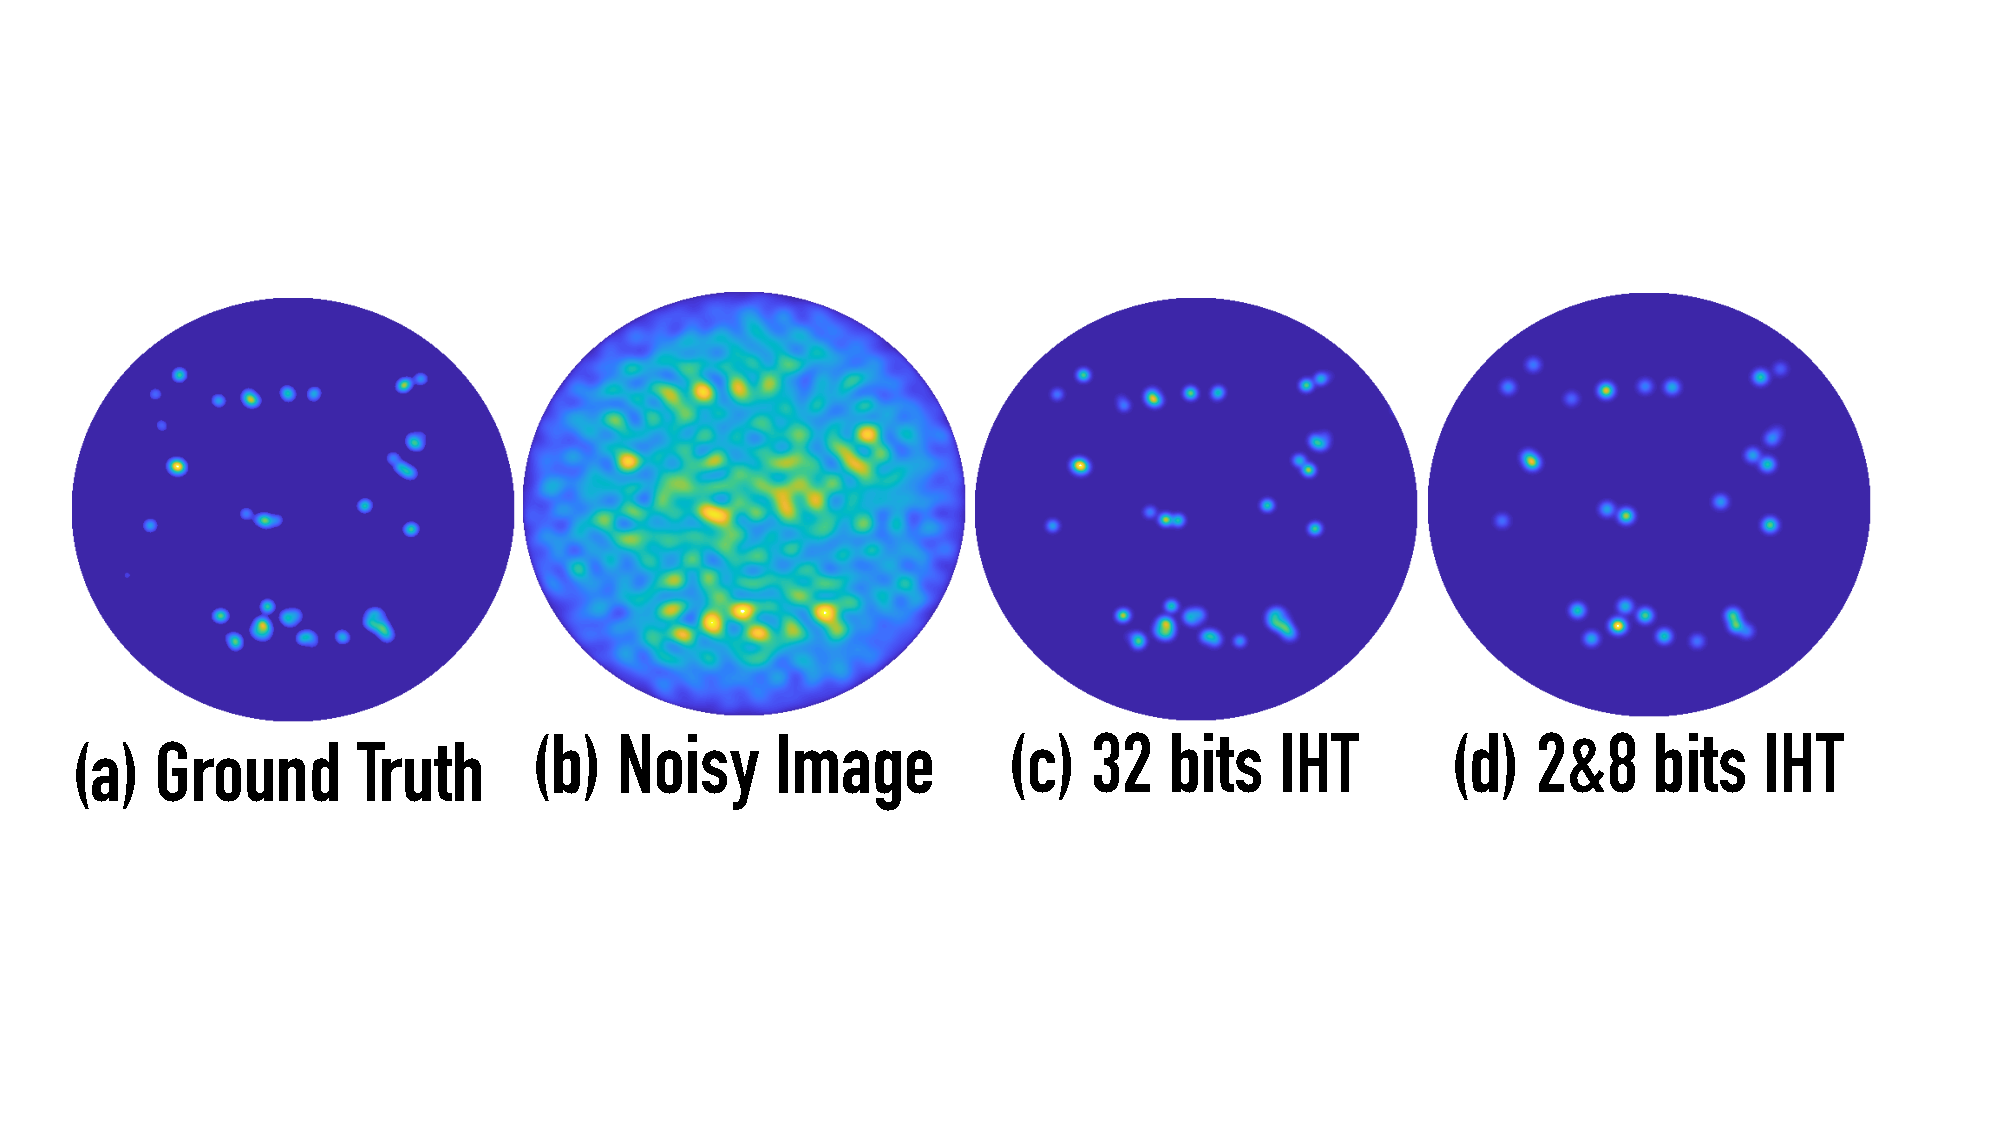
\includegraphics[width=1\textwidth]{figs/sky_images.pdf}
  %\caption{Sky recovery performances of high precision (32-bits), low precision (2-bits) IHT and CLEAN on a synthetic data setting populates with 30 celestial sources.}
  %\vspace{-2em}
  \caption{Illustration of the main results of this paper. Representing all input data at 
  low precision, Iterative Hard Thresholding gets negligible loss of recovery quality (data from LOFAR station CS302, 2 bit measurement matrix and 8 bit observation). This paper provides both  the analysis, and the system implementation.}
  \label{fig:sky_images}
\end{figure}
%This work proposes to reduce the precision of floating-point data representations by reducing the bit widths, hence enabling more information transfer and processed at the Central Signal Processor of telescope. We first linearize image acquisition process by formulating the problem in compressive sensing framework, and under certain constraints, derive near-optimal guarantees for precise sky recovery. Our approach is a general framework and can facilitate further sparse reconstruction problems demanding high processing capability in practice. We demonstrate the power of our proposal on LOFAR, where we achieve significant practical speedup.
%radio interferometry encounters the task of inferring from measured information
\vspace{0.5em}

%\vspace{-1em}
\subsection{Problem Formulation}

%\vspace{-0.5em}
Compressive sensing (CS)~\citep{donoho2006cs, candes2006cs, candes2006cs2} is a foundational technique in sparse signal reconstruction. CS offers a range of efficient algorithms acquiring high dimensional signals from inaccurate and incomplete samples with an underlying sparse structure. 
Many real-life problems, e.g, medical imaging, interferometry, video, spectroscopy and genomic data analysis, can benefit from these techniques.
\vspace{0.5em}

% 1- CS
In mathematical terms, CS is formulated as follows. Let a sparse or approximately sparse signal ${\bf x}\in \mathbb{R}^N$ be sampled via a linear sampling operator ${\bf \Phi}^{M\times N}$. In matrix notation, the vector of measurements ${\bf y} \in \mathbb{C}^M$ is
\begin{equation}\label{CS_model}
 {\bf y} =  {\bf \Phi}  {\bf x} + {\bf e}
\end{equation}
where ${\bf e}$ is the observation noise and $M < N$.
\vspace{0.5em}

CS recovery algorithms iteratively build up a sparse estimate ${\bf x}$ such that ${\bf \Phi}  {\bf x}$ approximates ${\bf y}$ well, that is,  $\| {\bf y}- {\bf \Phi}  {\bf x} \|_2$ is small. The sparsity constraint imposed on ${\bf x}$ overcomes this ill-posed problem, yet is computationally NP-hard due to its combinatorial nature. 
Therefore, most CS algorithms resort to convex relaxation of $\ell_0$-based optimization, or a collection of thresholding and greedy methods such as Iterative Hard Thresholding (IHT) \citep{blumensath2008iht, blumensath2009iht} and Compressive Sampling Matching Pursuit (CoSaMP) \citep{needel2008cosamp}. The past decade has seen significant work on such methods, see~\citep{liu2017dualiht, yuan2014ht, yuan2016htp, blumensath2013cs, needel2008cosamp} and references therein. These references present an comprehensive analysis of the provable performance guarantees for such sparsity-constrained minimization methods, in terms of convergence to fixed points of $\ell_0$-regularized cost functions and the optimality of such approximations. However, these frameworks face several challenges when applied to real-life problems: for provable guarantees, it is often required that (1) the measurement matrix ${\bf \Phi}$ satisfies the Restricted Isometry Property (RIP)~\citep{candes2008rip, chartrand2008rip}, and that (2) the sparsity level is chosen appropriately. 
Normalized IHT (NIHT)~ \citep{blumensath2010niht}, is a simple yet very effective strategy  which relieves some of the limitations listed above: a step size parameter is introduced to the traditional IHT~\citep{blumensath2008iht}. This simple refinement alleviates the RIP condition imposed on ${\bf \Phi}$, enabling rigorous guarantees for a broader class of practical problems. {This paper
builds upon this line of work.}

\vspace{.5em}
\paragraph*{Problem Formulation}
 We consider the sparse signal recovery problem in Eqn.~(\ref{CS_model}) described as: given ${\bf y}$ and ${\bf \Phi}$, find coefficients ${\bf x}$ minimizing the cost function
 \begin{equation}\label{cost_function}
     \|{\bf y} - {\bf \Phi x} \|_2^2 \ \ \rm{subject \ to \ \|{\bf x} \|_0 \leq s},
 \end{equation}
 where $\|{\bf x} \|_0 = |\rm{supp}({\bf x})| = |\{i: x_i\neq 0 \}|$.
 
\vspace{0.5em}
%\subsection{Technical contributions}

Under certain constraints, normalized IHT is guaranteed to approximate ${\bf x}$ with high accuracy. Here, we consider the properties of this algorithm in a lossy compression setting, where the data ${\bf y}$ and ${\bf \Phi}$ consisting of floating-point values undergo a stochastic quantization process to a small set of integer levels denoted by $Q$. The goal of $Q$ is to reduce the extremely high cost of data transmission. That is, we wish to recover ${\bf x}$ using the  modified NIHT update rule:
 \begin{equation}
     {\bf x}^{[n+1]} = H_s({\bf x}^{[n]} + \mu^{[n]}Q({\bf \Phi})(Q({\bf y}) - Q({\bf \Phi}){\bf x}^{[n]}))
 \end{equation}
where $H_s({\bf x}): \mathbb{C}^n \rightarrow \mathbb{C}^n$ the nonlinear operator that preserves the largest $s$ (in magnitude) entries of {\bf x} and sets the rest to zero. 
 
 % The core contribution of this work is two fold in theory and algorithm as highlighted in below: 
 %
 %    $\bullet$ Low precision IHT: we established a rigorous analysis on the quality of recovery by bounding the approximation error. To our knowledge, compression performed on the measurement matrix has not been reported elsewhere in liteature.\\
 %    $\bullet$ We formulate radio interferometry imaging as a CS problem and employed low precision IHT on a real telescope. Our experiments demonstrated that sky map can still be recovered with no or small accuracy lost by using only 2-bits to represent the data points with 7.7x speed-up on FPGA.
     
%{\bf Organization. }
%The rest of this paper is organized as follows. In Section \ref{section_related_work} we briefly review some relevant work. Section \ref{section_iht} serves an introduction to IHT, including the theoretical performance guarantees. Section~\ref{section_lpiht} describes how the low precision framework is applied to IHT and presents derivable theoretical guarantees for such a lossy scheme, and devises our approach for real telescopes. Section~\ref{section_experiments} reports the numerical evaluation results. Section~\ref{section_discussion} concludes the overview. All the technical proofs are deferred to the supplementary material.



\begin{figure}[t]
\small
\centering
\begin{tabular}{c|c|cc}
\hline
                   & Assumption on ${\bf \Phi}$ & $Q(\Phi)$ & $Q(y)$ \\
\hline
 Boufounos et al.
 & Gaussian  &$\times$ & $\checkmark$\\
 Ai et al.         & unit variance &$\times$ & $\checkmark$\\
 Jacques et al.     &  RIP & $\times$& $\checkmark$\\
 Laska et al.     & Gaussian \& RIP &$\times$ & $\checkmark$\\
 Plan et al. (2011)     & Gaussian \& RIP &$\times$ & $\checkmark$\\
 Plan et al. (2012)      & Gaussian &$\times$ & $\checkmark$\\
 Gupta et al.     & Gaussian &$\times$ & $\checkmark$\\
 Gopi et al.       & sub-Gaussian/binary \& RIP &$\checkmark$ & $\checkmark$\\
\hline
  {\bf This Paper}                & non-symmetric RIP & $\checkmark$ & $\checkmark$ \\
\hline
\end{tabular}
%\vspace{-1em}
\caption{Comparison of This Paper with Previous Work. $Q({\bf \Phi})$ and $Q({\bf y})$ means whether
the paper considers quantizing ${\bf \Phi}$ and $y$,
respectively ($\checkmark$ means yes).}
\label{tab:cs}
%\vspace{-2em}
\end{figure}



%\vspace{-1em}
\section{Related work}\label{section_related_work}
%\vspace{-0.5em}

Using a low precision data representation in the context of compressive sensing
is not new. In fact, a series of studies made successive attempts to apply low precision  
to compressive sensing problems, summarized in
Fig.~\ref{tab:cs}. \citep{boufounos20091bitcs} demonstrate that sparse signals can be recovered with a scale factor when measurements preserve only sign information. \citep{ai20121bitcs, davenport20121bit} show that approximately sparse signals can be robustly recovered from single-bit measurements sampled with a sub-Gaussian distribution. \citep{jacques20111bit, laska20111bitcs} study the similar setting with a Gaussian measurement matrix, the so called Binary IHT. \citep{plan20111bitcs, plan20121bitcs} propose a computationally tractable and optimal recovery of 1-bit compressive sensing problem. \citep{recht20121bitcs, gopi20131bitcs} present provable theoretical guarantees to identify support recovery of high dimensional sparse signals for 1-bit measurements. 
\vspace{0.5em}

{This paper differs from these references
in two ways: First, as we discuss in Section~\ref{section_lpiht},
our assumption that the measurement matrix being
non-symmetric RIP is critical in radio astronomy applications, 
and none of these assumptions made by previous work would fit  this use case. Second, we are the only work,
with the exception of~\citep{gopi20131bitcs}, that quantizes
{\em both} the measurement matrix $\Phi$ and the observations.
\citep{gopi20131bitcs} considers the problem of building a  binary measurement matrix which can provide good support recovery guarantees given only one-bit measurements; by contrast, we consider a practical setting where we must quantize a given full-precision measurement matrix as well as possible, and can trade off higher precision for better recovery guarantees. 
We discuss the system-side benefits  
of quantizing the matrix ${\bf \Phi}$ in Section~\ref{sec:fpga}. 

} 
\vspace{0.5em}

%\citep{recht20121bitcs} identifies the support of sparse signals by using binary measurements.

%\citep{gopi20131bitcs} studies 1 bit CS with rigorous support and approximation error: norm(x-xs) guarantee. The measurement matrix is designed using a Gaussian and the actual measurement matrix}

Another emerging line of work has been on low precision training for 
machine learning applications beyond compressive
sensing. Examples include Buckwild!~\citep{desa2015hogwild},
QSGD~\citep{alistarh2016qsgd},  
ZipML~\citep{zhang2017zipml}, and
a series of works about 
partial or end-to-end low-precision training 
of deep learning models~\citep{seide2014sgd1bit, hubara2016qsnn, rastegari2016binarycnn,zhou2016cnn, miyashita2016cnn, li2016twn, gupta2015dl}.
Most of these works are designed for stochastic gradient descent (SGD). In this paper, we 
go beyond SGD, and focus on  compressive sensing.


%Multi-level quantization of measurement for CS problems, therefore, exhibit a great empirical success. The analysis of such heuristics is yet challenging. In this paper, a successive application of low precision framework to CS, particularly IHT, is shown to possess rigorous theoretical guaratees, potentially allowing more efficient information processing in large scale applications. To distinct from the prior proposals listed above, we achieve this by quantizing not only measurements but also measurement matrix.

Another rich line of research is on 
designing efficient algorithms for sparse recovery problems~\citep{blumensath2011aiht, wei2015fiht, blanchard2013iht, cevher2011ht, liu2017dualiht}. We focus here on normalized IHT, and leave extensions to other recovery methods as future work.




%\vspace{-1em}
\section{Preliminaries}\label{section_iht}
%\vspace{-0.5em}

In this section, we review the preliminary results on the normalized IHT (NIHT) algorithm introduced by~\citep{blumensath2010niht, blumensath2012greedy}.
%\vspace{-0.3em}
\vspace{0.5em}

{\it Notation:} Scalars are denoted by italics, vectors by bold lower-case and matrices by bold upper-case. For all ${\bf x}= (x_1, \ldot, x_N) \in \mathbb{R}^N$, we denote by $\|{\bf x}\|_p$ the standard operator norm. Let ${\bf \Phi}_{m, n}\in \mathbb{C}^{M\times N}$ denote the matrix element in the $m$'th row and $n$'th column. Finally {\it 32 bit} denotes the full precision scheme and $b_{\bf \Phi}\&b_{\bf y}$ {\it bit} precision denote the number of bits used to represent the measurement matrix ${\bf \Phi}$ and vector of observations ${\bf y}$, respectively.
%\vspace{-1em}
\subsection{Iterative Hard Thresholding} 
%\vspace{-0.5em}
Let ${\bf x}^{[0]} = 0$. Normalized IHT has the following update rule per iteration: 
\begin{equation}\label{iht_update_rule}
{\bf x}^{[n+1]} = H_s({\bf x}^{[n]} + \mu^{[n]}{\bf \Phi}({\bf y}-{\bf \Phi}{\bf x}^{[n]})),
\end{equation}
where $\mu^{[n]}>0$ is the adaptive step size parameter, and $H_s({\bf x})$ is the
thresholding operator that preserves the largest $s$ (in magnitude) entries.



%Under certain conditions, the normalized IHT converges to a local minimum of the optimization problem
%\begin{equation}\label{cost_function}
%    \textrm{min} \|{\bf y}-{\bf \Phi x} \|_2^2
%\ \ \ {\textrm{subject \ to }}\ \ \|{\bf x}\|_0 \leq s.
%\end{equation}

\subsection{Convergence} 
The analysis of hard thresholding algorithms heavily relies on the scaling properties of ${\bf \Phi}$. More precisely, the convergence to a local minimum of the cost function Eqn.~\ref{cost_function} as well as the quality of such approximation are proven under certain conditions on ${\bf \Phi}$. More concretely, one must often deal with non-symmetric Restricted Isometry Property (RIP) condition: a matrix ${\bf \Phi}$ satisfies non-symmetric RIP if
\begin{equation}\label{rip}
\alpha_{s} \leq \frac{\|{\bf \Phi} {\bf x}\|_2}{\|{\bf x}\|_2} \leq \beta_{s}
\end{equation}
for all ${\bf x}: \|{\bf x}\|_0 \leq s$, and where $0<\alpha_s, \beta_s \in \mathbb{R}, \ \alpha_s\leq \beta_s$, the so-called Restricted Isometric Constants (RICs), are lower and upper singular values of ${\bf \Phi}$, respectively.

\begin{remark}\label{remark_noise_amp}
The convergence of normalized IHT depends conditionally on the step size parameter $\mu^{[n]}$, unlike the traditional IHT approach where $\mu^{[n]}=1$.
While the traditional approach requires a re-scaling of the measurement matrix such that $\|{\bf \Phi}\|_2 <1$ to ensure convergence, introducing a step size parameter enables the arbitrary scaling of ${\bf \Phi}$ hence relaxing the bounds on its norm. The role of $\mu^{[n]}$ here is to compensate for this re-scaling by accordingly avoiding the undesirable amplification of noise, i.e., the ratio $\|{\bf \Phi x}\|_2/\|{\bf e}\|_2$ remains unchanged. 
\end{remark}
%\vspace{-0.5em}
The main convergence result can be stated as follows.
\begin{theorem}\label{theorem_convergence_IHT}
{\rm{\citep{blumensath2012greedy}}}\\ 
Let ${\bf \Phi}$ be full rank, and $s\leq m$. If $\beta_{2s}\leq\mu^{-1}$, then NIHT converges to a local minimum of Eqn.~\ref{cost_function}.
\end{theorem}
%\vspace{-1em}
\subsection{Step Size Determination} 
%\vspace{-.5em}
When setting the step size parameter, the condition that $\beta_{2s}\leq\mu^{-1}$, which ensures convergence, poses the following challenge. To date, there is no universal strategy  to check if the RIP holds for an arbitrary measurement matrix in a computationally efficient manner. A similar discussion holds for attaining the RICs, i.e., ${\beta_s}$ and $\alpha_s$, associated with the measurement matrix ${\bf \Phi}$. It can however be shown that, under certain conditions, randomly constructed measurement matrices can satisfy
the RIP with high probability~\citep{candes2008rip, chartrand2008rip}. Still, this remains a bottleneck for a more general class of
measurement matrices. Without losing the main track, we briefly review generic strategies for step size determination. 
\vspace{0.5em}

If the support is fixed, a natural strategy to set the step size adaptively is~\citep{blumensath2010niht}
\begin{equation}\label{step_size}
   \mu^{[n]} = \frac{{\bf g}^T_{\Gamma^{[n]}}{\bf g}_{\Gamma^{[n]}}}{{\bf g}^T_{\Gamma^{[n]}}{\bf \Phi}^T_{\Gamma^{[n]}}{\bf \Phi}_{\Gamma^{[n]}}{\bf g}_{\Gamma^{[n]}}}
\end{equation}
where ${\bf g}^{[n]} = {\bf \Phi}^T({\bf y}-{\bf \Phi x}^{[n]})$. Clearly, the maximal reduction in cost function can then be attained. However, if the support of ${\bf x}^{[n+1]}$ differs from that of ${\bf x}^{[n]}$, the sufficient convergence condition  becomes
\begin{equation}
    \mu^{[n]} \leq(1-c) \frac{\|{\bf x}^{[n+1]}-{\bf x}^{[n]} \|_2^2}{\|{\bf \Phi}({\bf x}^{[n+1]}-{\bf x}^{[n]}) \|_2^2},
\end{equation}
for any small constant $c$.
\vspace{0.5em}

If the above condition is not met, a new proposal for ${\bf x}^{[n+1]}$ can be calculated by using $\mu^{[n]}\leftarrow{\mu^{[n]}/(k(1-c))}$, where $k$ is a shrinkage parameter such that $k>1/(1-c)$.
% In a series of papers [...], extensive research effors have been made and strong theoretical guarantees were derived. Here we state the most refined recovery error bounds.
This adaptive setting of step size parameter is shown to provide RIP-invariant convergence  as follows.

\begin{theorem}\label{guarantee_niht}
{\rm{\citep{blumensath2010niht}}}\\
Consider a noisy observation ${\bf y} = {\bf \Phi x} + {\bf e}$ with an arbitrary vector ${\bf x}$. If rank({${\bf \Phi}$}) = m and rank(${\bf \Phi}_{\Gamma}$) = s \ $\forall \Gamma:\ |\Gamma| = s$, then the normalized IHT algorithm converges to a local minimum of the cost function Eqn.~\ref{cost_function}. Also, assume ${\bf \Phi}$ is non-symmetric RIP$_{2s}$ and let $\gamma_{2s} = \beta_{2s}/\alpha_{2s}-1$. If $\gamma_{2s} \leq {1}/{8}$, then
\begin{equation}
    \| {\bf x}-{\bf x}^n\|_2 \leq 2^{-n}\| {\bf x}^s\|_2 + 8 {{\bf \epsilon}_s}\label{niht_error_bound}
\end{equation} where \begin{equation}
     {{\bf \epsilon}_s} =  \| {\bf x}-{\bf x}^s\|_2 + \frac{\| {\bf x}-{\bf x}^s\|_1}{\sqrt{s}}+\frac{1}{\beta_{2s}}\|{\bf e} \|_2.
\end{equation}
After at most $n^*=\log_2(\|{\bf x}^s\|_2/ {\bf \epsilon}_s)$ iterations, the recovery error bound in Eqn.~\ref{niht_error_bound} can be further simplified to
\begin{equation}
   \| {\bf x}-{\bf x}^n\|_2 \leq 9 {{\bf \epsilon}_s}.
\end{equation}
\end{theorem}
The above result suggests that, after a sufficiently large number of iterations, the reconstruction error is induced only by the noise ${\bf e}$ and that ${\bf x}$ is not exactly s-sparse.

%\vspace{-1em}
\section{Low Precision Iterative Thresholding}\label{section_lpiht}
%\vspace{-0.5em}

In this section, we analyze the
quantized version of IHT for 
its guarantee for signal recovery performance.
The key development here is that, by reducing the bit widths of the data points in a structured manner, we
can upper bound the recovery error. 
In Section~\ref{section_experiments},
we will show that for radio astronomy,
we expect this error to be small, given
the structure of the measurement matrix.

As introduced earlier, let ${\bf x}^{[0]} = 0$ and use the iteration
\begin{equation} \label{modified_update_rule}
  {\bf x}^{[n+1]} = H_s\big({\bf x}^{[n]}+\hat{\mu}^{[n]} Q_b(\boldsymbol{\Phi})(Q_b({\bf y})-Q_b(\boldsymbol{\Phi}){\bf x}^{[n]})\big)  
\end{equation}
where $Q(\cdot)$ is the quantization function that maps single-precision floating-point values onto a co-domain where each element has $b$-bits precision.

\vspace{0.5em}
{\bf Quantization Scheme:} We analyze a stochastic quantization function denoted with $Q_b({\bf v})$, where ${\bf v}=(v_1, v_2, .., v_d) \in \mathbb{R}^d$ is an arbitrary vector and $b$ is the total number of bits used to represent it. ${\bf v}$ can then be quantized into $l=2^b$ levels as follows. Let $\ell_i$, $i\in \{1, 2, ..., l-1 \}$ denote $l$ equally spaced points on $[-1, 1]$ such that $\ell_1= -1$, $\ell_l= +1$ and $\ell_1\leq\ell_2 \leq ... \leq \ell_l$, also $v_j$ for $j\in \{1, 2, ..., d \}$ fall into the interval $[\ell_i, \ell_{i+1}]$. Then we assign the probabilities to the nearest levels as
\[
    Q_b(v_j) = \left\{\begin{array}{lr}
        \ell_i, & \textrm{with probability} \ \frac{\ell_{i+1}-v_j}{\ell_{i+1}-\ell_i}\\
        \ell_{i+1},&\textrm{otherwise}.  \ \ \ \  \ \ \ \ \ \ \ \ \ \ \ \ \ \ 
        \end{array}
\]
  
It follows that the quantization operation $Q(\cdot)$ is unbiased, i.e., $\mathbb{E}[Q_b({\bf v})] = {\bf v}$. Also, let $\hat{{\bf v}}$ represent the quantized ${\bf v}$ and drop $Q_b(\cdot)$ to simplify notational burden. The detailed steps of the algorithm are given in Algorithm \ref{low_precision_iht}.

\vspace{0.5em}
{\bf Deterministic Quantization:} A slightly more efficient compression scheme is via deterministic quantization, i.e., quantize the number
$v_j \in [\ell_i, \ell_{i+1}]$ directly to the nearest
value, either $\ell_i$ or $\ell_{i+1}$. 
This quantization scheme will lead to the same 
error bound and similar empirical result as stochastic quantization. {We leave the analysis
of this case to the supplementary material.}


\begin{algorithm}[t!]
   \small
   \caption{Low Precision Iterative Thresholding}
   \label{low_precision_iht}
\begin{algorithmic}
   \STATE {\bfseries Input:} The set of low precision measurement matrices $\{ \hat{\bf \Phi}_1, \hat{\bf \Phi}_2, ...\hat{\bf \Phi}_{2n^*}\}$, measurements $\hat{\bf y}$, sparsity parameter $s$, number of iterations $n^*$, step size tuning parameters {\it k,\ c} 
  % \REPEAT
   \STATE Initialize ${\bf x}^{[0]} = 0$, $\Gamma^{[1]} = \rm{supp}\big (H_s(\hat{\bf \Phi}_1^{\dagger}{\hat{\bf y}})\big)$.
   \FOR{$n=1$ {\bfseries to} $n^*$}
   \STATE ${\bf g}^{[n]} = {\hat{\bf \Phi}}_{2n-1} \big(\hat{{\bf y}}-{\hat{\bf \Phi}}_{2n}{\bf x}^{[n]}\big)$
   \STATE $\hat{\bf \mu}^{[n]} = ({\bf g}^{\dagger}_{\Gamma^{[n]}}{\bf g}_{\Gamma^{[n]}})/({\bf g}^{\dagger}_{\Gamma^{[n]}}{\bf \Phi}^{\dagger}_{\Gamma^{[n]}}{\bf \Phi}_{\Gamma^{[n]}}{\bf g}_{\Gamma^{[i]}})$
   \STATE ${\bf x}^{[n+1]} = H_s({\bf x}^{[n]} + \hat{\bf \mu}^{[n]} {\bf g}^{[n]})$
   \STATE $\Gamma^{[n+1]} = \rm{supp}({\bf x}^{[n+1]})$\\
   \algorithmicif{  \ $\Gamma^{[n+1]}=\Gamma^{[n]}$}
   \STATE \ \ \ \ ${\bf x}^{[n+1]}=\bf x}^{[n]}$\\
   \algorithmicelse \ \algorithmicif{\ $\Gamma^{[n+1]}\neq \Gamma^{[n]}$}\\
   \STATE \ \ \ \ ${ b}^{[n]}=(\|{\bf x}^{n+1}-{\bf x}^{n} \|^2_2)/(\|\hat{\bf \Phi}_{2n-1}({\bf x}^{n+1}-{\bf x}^{n})\|^2_2)$\\
   \ \ \ \ \algorithmicif{\ { $\hat{\mu}^{[n]}\leq (1-{c})b^{[n]}$ }}
   \STATE \ \ \ \ \ \ \ {${\bf x}^{[n+1]}=\bf x}^{[n]}$}\\
   \ \ \ \ \algorithmicelse {  $\hat{\mu}^{[n]}>(1-{c})b^{[n]}$}
   \STATE \ \ \ \ \ \ \ {\bf repeat} \ {$\hat{\mu}^{[n]} \leftarrow \hat{\mu}^{[n]}/(k(1-c))$}
   \STATE \ \ \ \ \ \ \ ${\bf x}^{[n+1]} = H_s({\bf x}^{[n]} + \hat{\bf \mu}^{[n]} {\bf g}^{[n]})$
   \STATE \ \ \ \ \ \ \ {\bf until} \ {$\hat{\mu}^{[n]}\leq (1-{c})b^{[n]}$ }
   \STATE $\Gamma^{[n+1]} = \rm{supp}({\bf x}^{[n+1]})$
   \ENDFOR
  % \UNTIL $n = n^*$
\end{algorithmic}
\end{algorithm}


% \begin{algorithm}[tb]
%   \caption{Low Precision Iterative Thresholding}
%   \label{low_precision_iht}
% \begin{algorithmic}
%   \STATE {\bfseries Input:} The set of low precision measurement matrices $\{ \hat{\bf \Phi}_1, \hat{\bf \Phi}_2, ...\hat{\bf \Phi}_{2n^*}\}$, measurements $\hat{\bf y}$, sparsity parameter $s$, number of iterations $n^*$ 
%   \REPEAT
%   \STATE Initialize ${\bf x}^{[0]} = 0$, $\Gamma^{[1]} = \rm{supp}\big (H_s(\hat{\bf \Phi}_1^{\dagger}{\hat{\bf y}})\big)$
%   \FOR{$n=1$ {\bfseries to} $n^*$}
   %\STATE ${\bf g}^{[n]} = {\hat{\bf \Phi}}_{2n-1} \big ( \hat{\bf y}-\hat{\bf \Phi}_{2n}{\bf x}^{[n]}\big )$
%   \STATE $\hat{\bf \mu}^{[n]} = ({\bf g}^{\dagger}_{\Gamma^{[n]}}{\bf g}_{\Gamma^{[n]}})/({\bf g}^{\dagger}_{\Gamma^{[n]}}{\bf \Phi}^{\dagger}_{\Gamma^{[n]}}{\bf \Phi}_{\Gamma^{[n]}}{\bf g}_{\Gamma^{[i]}})$
%   \STATE ${\bf x}^{[n+1]} = H_s({\bf x}^{[n]} + \hat{\bf \mu}^{[n]} {\bf g}^{[n]})$
%   \STATE $\Gamma^{[n+1]} = \rm{supp}({\bf x}^{[n+1]})$
%   \IF{$\Gamma^{[n+1]}=\Gamma^{[n]}$}
%   \STATE ${\bf x}^{[n+1]}=\bf x}^{[n]}$
%   \IF{$\Gamma^{[n+1]}=\Gamma^{[n]}$}
%   \STATE ${\bf x}^{[n+1]}=\bf x}^{[n]}$
%   \ENDIF
%   \STATE $noChange = false$
%   \ENDIF
%   \ENDFOR
%   \UNTIL{$noChange$ is $true$}
% \end{algorithmic}
% \end{algorithm}


\vspace{0.5em}

{\bf Convergence:} The modified algorithm attains a local minimum of the cost function $\mathbb{E} [ \| \hat{\bf y} - \hat{\bf \Phi}{\bf x}\|_2^2]$ such that $\|{\bf x}\|_0 \leq s$. This can be majorized by the following surrogate objective function 
\begin{equation*}
    \begin{split}
        \mathbb{E} [\|\mu^{0.5}\hat{\bf y} -   \hat{\bf \Phi}{\bf x}\|_2^2+ \|{\bf x} 
    - {\bf x}^{[n]} \|_2^2
    - \|\mu^{0.5}\hat{\bf \Phi}({\bf x}- {\bf x}^{[n]}) \|_2^2] 
    \end{split}
\end{equation*}
whenever $\| \mu^{0.5}\hat{\bf \Phi}\|_2^2 <1$. If this condition is met, the minimizer of the above surrogate objective: ${\bf x}^{[n+1]}$ ensures that $\mathbb{E} [\| \hat{\bf y} - \hat{\bf \Phi}{\bf x}^{[n+1]}\|_2^2] \leq \mathbb{E}[ \| \hat{\bf y} - \hat{\bf \Phi}{\bf x}^{[n]}\|_2^2]$. Moreover, by using the arguments of~\citep{blumensath2008iht}, Eqn.~\ref{modified_update_rule} can be shown to minimize the expected cost $\mathbb{E} [ \| \hat{\bf y} - \hat{\bf \Phi}{\bf x}\|_2^2]$. For deterministic quantization scheme, Theorem~\ref{theorem_convergence_IHT} ensures the convergence to a fixed point. {We
will provide an analysis of the performance guarantee,
instead of only convergence.}
\vspace{0.5em}

%{\bf Computational Complexity:} The iterative thresholding algorithm involves two vector additions and two dense matrix multiplication as well as a thresholding operation per iteration, and this is doubled due to step size search. Low precision approach however reduces memory requirements significantly. (we need to improve here)
 
{\bf Conditions on ${\Phi}$:} The restricted isometry property holds for the quantized measurement if
\begin{equation}
    \hat{\alpha}_{s} \leq \frac{\|\hat{{\bf \Phi}} {\bf x}\|_2}{\|{\bf x}\|_2} \leq \hat{\beta}_{s}
\end{equation}
$\forall {\bf x}: \| {\bf x}\|_0 \leq s$. Furthermore, the RICs $\hat{\alpha}_s$ and $\hat{\beta}_s$ can be re-scaled accordingly with $\hat{\bf \Phi}$.

%{\bf Bounds of $\$:} 
%The step size $\hat{\mu}^{[n]}$ is required to counteract the scaling of $\hat{{\bf \Phi}}$ such that $\|\hat{\mu}^{0.5} \hat{\bf\Phi}\|_2^2 <1$ to ensure the convergence. 
%This adaptive step size setting yields the trivial bound on $\mu$ as~\citep{blumensath2012greedy}
%\begin{equation}
 %  1/\hat{\beta}_{2s}^2\leq  1/\hat{\beta}_s^2 < \hat{\mu}^{[n]} < 1/\hat{\alpha}_s^2 \leq 1/\hat{\alpha}_{2s}^2.
%\end{equation}
%Moreover, using \ref{step_size} in the low precision setting, we can initially determine $\hat{\mu}^{[n]}$ to guarantee the convergence without requiring the knowledge of the restricted isometry constants.
%\vspace{-.8em}
\subsection{Performance Guarantees}
%\vspace{-0.5em}
The recovery performance of such algorithms is of our primary interest. The following theorem states the recovery error by explicitly exhibiting the component introduced by the quantization.

\begin{theorem}\label{main_theorem_TH}
Given a noisy observation ${\bf y} = {\bf \Phi x}+{\bf e} $ where ${\bf y} \in \mathbb{C}^M$, ${\bf \Phi} \in \mathbb{C}^{M\times N}$ and ${\bf x} \in \mathbb{R}^N$ is an arbitrary vector with $\|{\bf x} \|_0 \leq s$. Let $H_s({\bf x}) = {\bf x}^s$ with $s\leq M$. Assume ${\bf \Phi}$ and $\hat{\bf \Phi}$ satisfy the non-symmetric RIP with ${\alpha}_s, {\beta}_s$ and $\hat{\alpha}_s, \hat{\beta}_s$ where ${\gamma}_{2s} = {\beta}_{2s}/{\alpha}_{2s} -1 \leq 1/16$ and $\hat{\gamma}_{2s} = \hat{\beta}_{2s}/\hat{\alpha}_{2s} -1 \leq 1/16$, respectively. If the normalized IHT algorithm is used at low precision we have
\begin{equation}\label{main_theorem}
\begin{split}
        \mathbb{E}[\|\hat{{\bf x}}^{[n+1]}-{\bf x}^s\|_2]  
        \leq &2^{-n}\|{\bf x}^{s}\|_2  + 10 {\epsilon}_s + 5 {\epsilon}_q
\end{split}
\end{equation}
with 
\begin{equation}
 {\epsilon}_s = \frac{1}{\beta_{2s}}\|{\bf e} \|_2 +\bigg  [ \|{\bf x}-{\bf x}^s \|_2 + \frac{\|{\bf x}-{\bf x}^s \|_1}{\sqrt{s}}\bigg]    
\end{equation}
and
\begin{equation}
 {\epsilon}_q = \frac{\sqrt{M}}{\hat{\beta}_{2s}}\Big ( \frac{\| {\bf x}^s\|_2}{2^{b_{\bf \Phi}-1}}+\frac{1}{2^{b_{\bf y}-1}} \Big )
\end{equation}
where $b_{\bf \Phi}$ and $b_{\bf y}$ are the numbers of bits used to represent ${\bf \Phi}$ and ${\bf y}$, respectively.
\end{theorem}
%\vspace{-.5em}
A natural stopping criterion is $n^* = \lceil \log_2 (\|{\bf x}^s \|_2/\epsilon_s)\rceil$, where the algorithm computes a successive approximation of ${\bf x}^s$ with accuracy
\begin{equation}
    \mathbb{E}[\|{\bf x}^{[n^*]}-{\bf x}^s \|_2] \leq 11\epsilon_s + 5\epsilon_q.
\end{equation}
The error bound above is slightly simplified; our proof in the supplementary material is slightly more delicate. Specifically, the quantization operator introduces only $\frac{5}{\beta
{2s}} \|{\bf e} \|_2$ into $8 {\epsilon}_s$ in Eqn.~\ref{niht_error_bound}, tighter than the $10 {\epsilon}_s$ in Eqn.~\ref{main_theorem}.

%\vspace{-.5em}
\subsection{Discussion and Limitations}
%\vspace{-0.5em}

We now examine the error bound presented in Theorem~\ref{main_theorem_TH}. Low precision IHT will asymptotically provide a sparse approximation of ${\bf x}$ up to the multiples of $ {\epsilon}_s$ and $ {\epsilon}_q$ involving the noise term ${\bf e}$, the approximation error on how well ${\bf x}$ can be represented by a sparse vector ${\bf x}^s$ and the noise introduced by the quantization operator. 
Here we highlight the properties, and stress the limitations of this approach.
%\vspace{-.3em}
\vspace{0.5em}

{\bf Condition on $\hat{\boldsymbol{\gamma}}_{2s}$:} In comparison to the unmodified algorithm, the condition under which the performance guarantee holds is stricter in our approach, i.e., ${\gamma}_{2s}, \hat{\gamma}_{2s}\leq 1/16$ where it was ${\gamma}_{2s}\leq 1/8$ in Theorem \ref{guarantee_niht}. In practice, this can be altered with a suitable transformation of $\hat{\bf \Phi}$ such that ${\gamma}_{2s}, \hat{\gamma}_{2s}\leq 1/16$ is satisfied. Alternatively, a closer look into the derivation in the supplementary material reveals that there exist finite constants $c_1$ and $c_2$ with $c_1\leq 11$ and $c_2\leq 5$ such that $\mathbb{E}[\|{\bf x}^{n^*}-{\bf x}^s \|_2] \leq c_1\epsilon_s + c_2\epsilon_q$ when ${\gamma}_{2s}, \hat{\gamma}_{2s}\leq 1/8$. For a wide class of problems, an accurate approximation of ${\bf x}^s$ can still be recovered after sufficient number of iterations.
%One might argue that it can potentially amplify noise yet from changing $\gamma_{2s}$ from $1/8$ to $1/16$ 
%\vspace{-.3em}
\vspace{0.5em}

%We also monitor $\hat{\gamma}_{2s}$ by using the strategy described in ref.
%can easily be verified in a computationally efficient manner
{\bf Natural limitations on ${\boldsymbol{\beta}}_{2s}$ and $\hat{\boldsymbol{\beta}}_{2s}$:} In both the low and full precision settings, the measurement matrix ${\bf \Phi}$ is scale-invariant, and rigorous theoretical guarantees are achievable provided its scaling onto sparse vectors is confined in certain intervals, i.e., ${\gamma}_{2s}, \hat{\gamma}_{2s}\in [0, 1/16]$. As discussed in Remark \ref{remark_noise_amp}, even if this condition is met, there still remains a further limitation by the noise ${\bf e}$. That is, the signal-to-noise ratio of $\|\hat{\bf \Phi} {\bf x} \|_2/\|{\bf e} \|_2$ will be amplified upon a down-scaling of $\hat{\bf \Phi}$. Re-scaling ${\bf y}$ could accordingly overcome this up to some level. 

%\vspace{-.3em}
\vspace{0.5em}
{\bf Further limitations on ${\boldsymbol{\beta}}_{2s}$ and $\hat{\boldsymbol{\beta}}_{2s}$ due to quantization:} The recovery error bound satisfying Eqn.~\ref{main_theorem} depends on the error term of full precision IHT: $ {\epsilon_s}$ and the quantization error: $ {\epsilon}_q$ that are inversely proportional to ${\beta}_{2s}$ and $\hat{\beta}_{2s}$, respectively. For sufficiently large values, which compensate for $\|{\bf e}\|_2$ and $\sqrt{M} \|{\bf x}^s \|_2$, the low precision approach appears competitive with the unmodified algorithm where the recovery error is bounded by $9\epsilon_s$ in Eqn.~\ref{niht_error_bound}. Furthermore, the scaling-invariant property of the measurement matrix ${\bf \Phi}$ permits us to scale up ${\beta}_{2s}$, hence $\hat{\beta}_{2s}$, by still retaining the strong recovery result similar to that of the full precision algorithm. An arbitrary scaling of ${\bf \Phi}$ has no effect on the condition ${\gamma}_{2s}, \hat{\gamma}_{2s}\leq 1/16$. We however have strong theoretical guarantees for recovery if the low precision algorithm operates in a regime where ${\gamma}_{2s}, \hat{\gamma}_{2s}\leq 1/16$ holds and ${\epsilon}_s$  and ${\epsilon}_q$ are small.
%\vspace{-.3em}

From the  point of view of quantization, re-scaling ${\bf y}$ and ${\bf \Phi}$ is not necessary. A small factor weightening ${\epsilon}_q$ naturally reduces the quantization error, yet imposes some mild conditions on $\hat{\beta}_{2s}$. Namely, $\hat{\beta}_{2s}$ can not be arbitrary: instead, it is required to satisfy that all entries of $\hat {\bf y}$ and $\hat{\bf \Phi}$ are contained in $[-1, 1]$.
%\vspace{-.3em}

% \subsection{An Alternative Approach}
% The normalized IHT offers an adaptive step size tuning to ensure maximal reduction in the cost function at each iteration, yet doubling the computational cost. We instead propose using a constant step size that guarantees the convergence, that is, $\hat{\mu}=\frac{k}{\|{\bf \Phi} \|_{\mathcal{F}}}$ with $0<k<1$. This modification might increase the convergence time but counteracts the additional cost introduced by iterative tuning of ${\mu}^{[n]}$. We therefore have the following version.
% \begin{theorem}
% Let ${\bf \Phi}$ satisfies the non-symmetric RIP with RICS $\alpha_s$ and $\beta_s$. If normalized IHT uses a constant step size $\mu = 1/(8\beta_{2s})$ then
% \begin{equation}\label{secondary_theorem}
% \begin{split}
%         \mathbb{E}[\|\hat{{\bf x}}^{[n+1]}-{\bf x}^s\|_2]  
%         \leq &2^{-n}\|{\bf x}^{s}\|_2  + 10 {\epsilon}_s + 5 {\epsilon}_q
% \end{split}
% \end{equation}
% with 
% \begin{equation}
%  {\epsilon}_s = \frac{1}{\beta_{2s}}\|{\bf e} \|_2 +\bigg  [ \|{\bf x}-{\bf x}^s \|_2 + \frac{\|{\bf x}-{\bf x}^s \|_1}{\sqrt{s}}\bigg]    
% \end{equation}
% and
% \begin{equation}
%  {\epsilon}_q = \frac{\sqrt{m}}{\hat{\beta}_{2s}}\Big ( \frac{\| {\bf x}^s\|_2}{2^{b_{\bf \Phi}-1}}+\frac{1}{2^{b_{\bf y}-1}} \Big )
% \end{equation}
% \end{theorem}
\vspace{0.5em}

{\bf Comparison to other state-of-art methods:} The compressive sensing literature covers a range of algorithms,  such as $\ell_1$-minimization, greedy and thresholding-based methods, each with its own trade-offs. In~\citep{blumensath2010niht}, CoSaMP, normalized IHT and $\ell_1$-minimization exhibit similar empirical performance when applied to the problems with dense Gaussian matrices. Moreover, after a simple modification of step size parameter, IHT has became compatible with these powerful methods with similar provable guarantees~\citep{blumensath2012greedy}. 
In the supplementary material, we show the  
empirical performance of low precision IHT on such synthetic examples using  Gaussian measurement matrices.



%\vspace{-0.5em}
\subsection{Radio Astronomy Application}
%\vspace{-0.5em}

In our application, radio interferometers at various locations on the ground record radio waves emitted by the celestial sources over a certain time interval, then store and process these signals to deduce a sky image. Interferometers first estimate the cross-correlation between the time series measurements, called visibilities, and the sky image is estimated by the so-called {CLEAN} algorithm~\citep{hogbom1974clean}. {CLEAN} is a greedy pursuit technique, deconvolving the inverse Fourier transform of visibilities and forming a sky map by iteratively removing a fraction of the highest peak, convolved with an instrument based point spread function. CLEAN is a simple and easy-to-implement imaging technique. However radio interferometers are also phrased as a CS problem, for example, by~\citep{wiaux2009csforra, wenger2010csforra, li2011deconvolution} because of their recovery success in noisy environments.
%\vspace{-.3em}
\vspace{0.5em}

Assume the sky is observed by employing $L$ antennas over a stationary time interval where the earth rotation is negligible. Denote the vectorized sky image by ${\bf x} \in \mathbb{R}^N$ with $N = {r^2}$ where $r$ is the resolution of images, i.e., height and width of the image in pixels. We formulate the interferometer pipeline as a compressive sensing problem such that ${\bf y} = {\bf \Phi} {\bf x} + {\bf e}$ where ${\bf \Phi} \in \mathbb{C}^{M\times N}$ is the measurement matrix with complex entries as a function of inner product between antenna and pixel locations, ${\bf y} \in \mathbb{C}^{M}$ is the visibilities where $M=L^2$, and ${\bf e} \in \mathbb{C}^M$ is the noise vector. For more background on the radio interferometer pipeline and formation of ${\bf \Phi}$, please see Section 3 of the supplementary material.

\vspace{0.5em}
{\bf Why iterative hard thresholding?} According to our formulation, the measurement vector ${\bf y}$ represents the cross-correlations between the antenna measurements: the visibilities. The naive method to map from ${\bf y}$ to a vectorized sky image ${\bf x}$ is the Fourier inversion followed by the {CLEAN} algorithm. Alternatively, {A(W)-projection} algorithm initially makes corrections on the visibilities then deduces a sky image~\citep{bhatganar2008ra}. Still, forming a sky map using the non-uniform samples of visibility functions recorded by finite number of antennas is naturally inaccurate. Furthermore, the thermal noise introduced by the electronic instruments embedded in the RF antenna receivers heavily corrupt the weak incoming signal, and therefore pose a further challenge for these imaging algorithms. To date, the current techniques revolve around carrying out noise reduction by collecting lots of data, so that the noise can be circumvented. The choice of IHT can be justified by its robustness to noise. We demonstrate this in detail, via further experiments in the supplementary material, where we show that the baseline {CLEAN} approach often resolves noise artefacts as actual sky sources. 
%\vspace{-.1em}
\vspace{0.1em}

We refine our error bound for the radio astronomy scenario:
%\vspace{-.2em}

\begin{corollary}
Let $\sigma_n^2$ is the variance of noise introduced by a single antenna. By Theorem \ref{main_theorem_TH}, if ${\gamma}_{2s}, \hat{\gamma}_{2s}\leq 1/16$, the low precision iterative hard thresholding recovers the sky image ${\bf x}^s$ with accuracy
\begin{equation}
    \mathbb{E}[\|{\bf x}^{n+1} - {\bf x}^s \|_2] \leq 2^{-n}\| {\bf x}^s\|_2 + 10(\frac{\sqrt{L}}{\beta_{2s}}\sigma_n+\frac{L}{\hat{\beta}_{2s}}\epsilon_{\rm{sky}})
\end{equation}
where $\epsilon_{\rm{sky}} =  \|{\bf x}^s \|_2/2^{b_{\bf \Phi}} + 1/2^{b_{\bf y}}$.
\label{corollary1}
\end{corollary}

%The above finding suggest that the sky image can be recovered with high accuracy when $\hat{\beta}_{2s}$ is sufficiently small. This will further be demonstrated in Section~\ref{section_experiments}.

%real life problems generally not known, whether the conditions are satisfied or not

{\bf Discussion: LOFAR and Beyond.}
Corollary~\ref{corollary1} shows that the sky image 
can be recovered with high accuracy when certain conditions  hold:
${\beta}_{2s}$ and $\hat{\beta}_{2s}$ are sufficiently large, ${\gamma}_{2s}$ and $\hat{\gamma}_{2s}$
are sufficiently small. Do these conditions hold for a real telescope? We now analyze it for one station of the LOFAR telescope, and discuss it further for radio interferometers in general.

% Real-life problems usually lack of traditional RIP, that is, $\|{\bf \Phi}\|_2 < 1$. The scale-invariant feature of the measurement matrix used in normalized IHT however alleviates the RIP condition and imposes a fairly mild constraint in~\ref{rip_lowprecision}, i.e., non-symmetric RIP. In a series of paper~\citep{blumensath2010niht, blumensath2012greedy}, CoSaMP is shown to perform markedly worse when the RIP condition fails. IHT, however, still preserves its near-optimal recoveries far beyond the region of RIP. While this favors IHT over CoSaMP when applying to real-life problems, there is no rigid assumption imposed on $\ell_1$-minimization. Still \ref{rip} trivially holds.
% \begin{figure}[h!]
% \centering
% 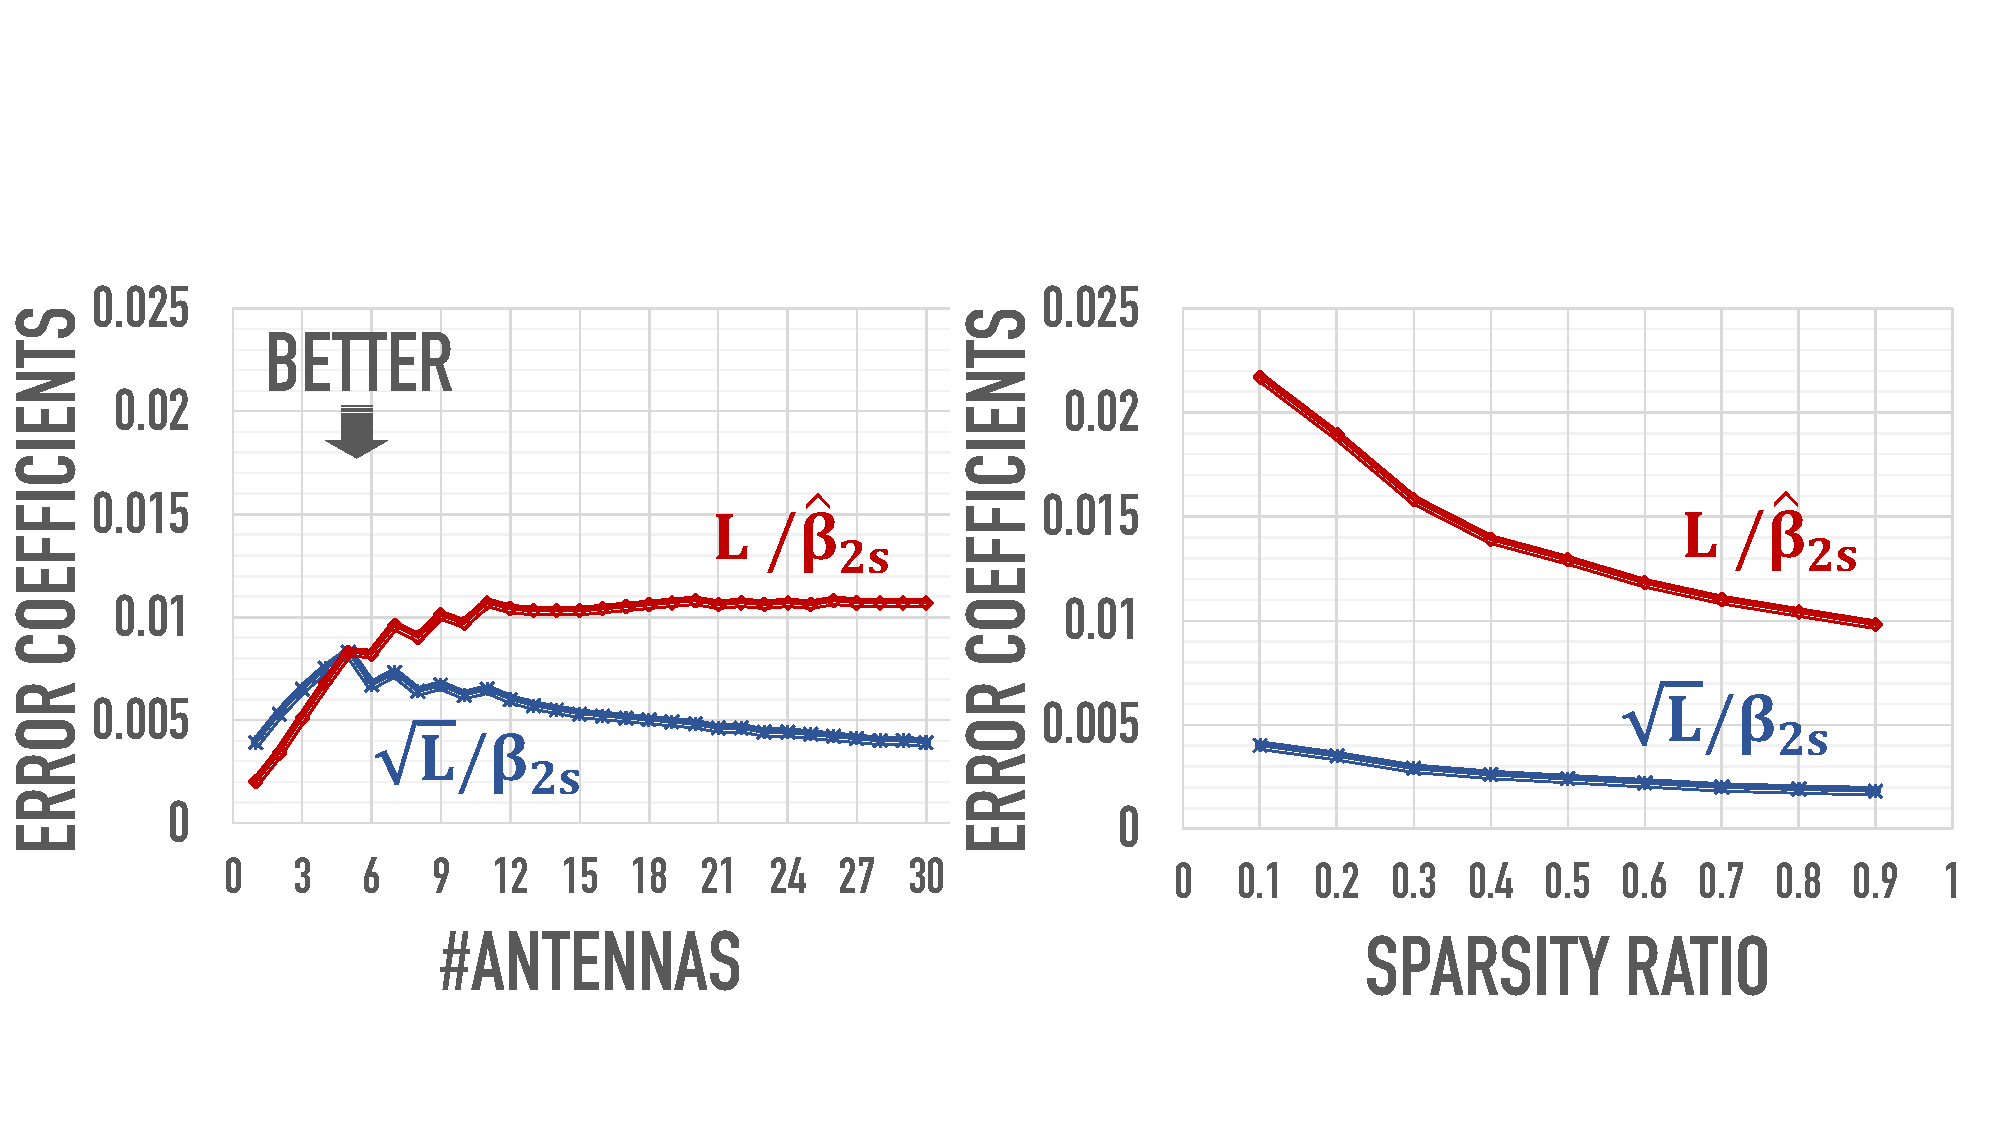
\includegraphics[width=1\columnwidth, angle=0]{figs/beta.pdf}
% \caption{Monitoring the error coefficients: $1/\beta_{2s}$ and $L/\hat{\beta}_{2s}$ that scale $ {\epsilon}_s$ and $ {\epsilon}_q$, respectively. Sparsity ratio stands for $2s/M$. The numerical value of coefficients guarantees that quantization error $ {\epsilon}_q$ is sufficiently small regardless of the number of bits used to represent ${\bf \Phi}$.}
% \label{fig:beta}
% \end{figure}
%\vspace{-.1em}
\vspace{0.5em}

 Recall from Theorem~\ref{main_theorem_TH} the two conditions ensuring  performance guarantees: (a) $\gamma_{2s}, \hat{\gamma}_{2s} \leq 1/16$, (b) ${L}/{\hat{\beta}_{2s}}$ must be large to minimize quantization error $ {\epsilon}_q$. Fortunately, in the radio interferometry application, the image grid we initially form as well as scale-invariant property of normalized IHT yield us the control over $\gamma_{2s}, \hat{\gamma}_{2s}$ and ${\beta}_{2s}, \hat{\beta}_{2s}$, respectively, through a pre-processing of ${\bf \Phi}$. Analytic derivations of these parameters are possible in theory, but intractable due to amount of nonlinear operations contained in the formulation of ${\bf \Phi}$. 
\begin{figure}[t!]
\centering
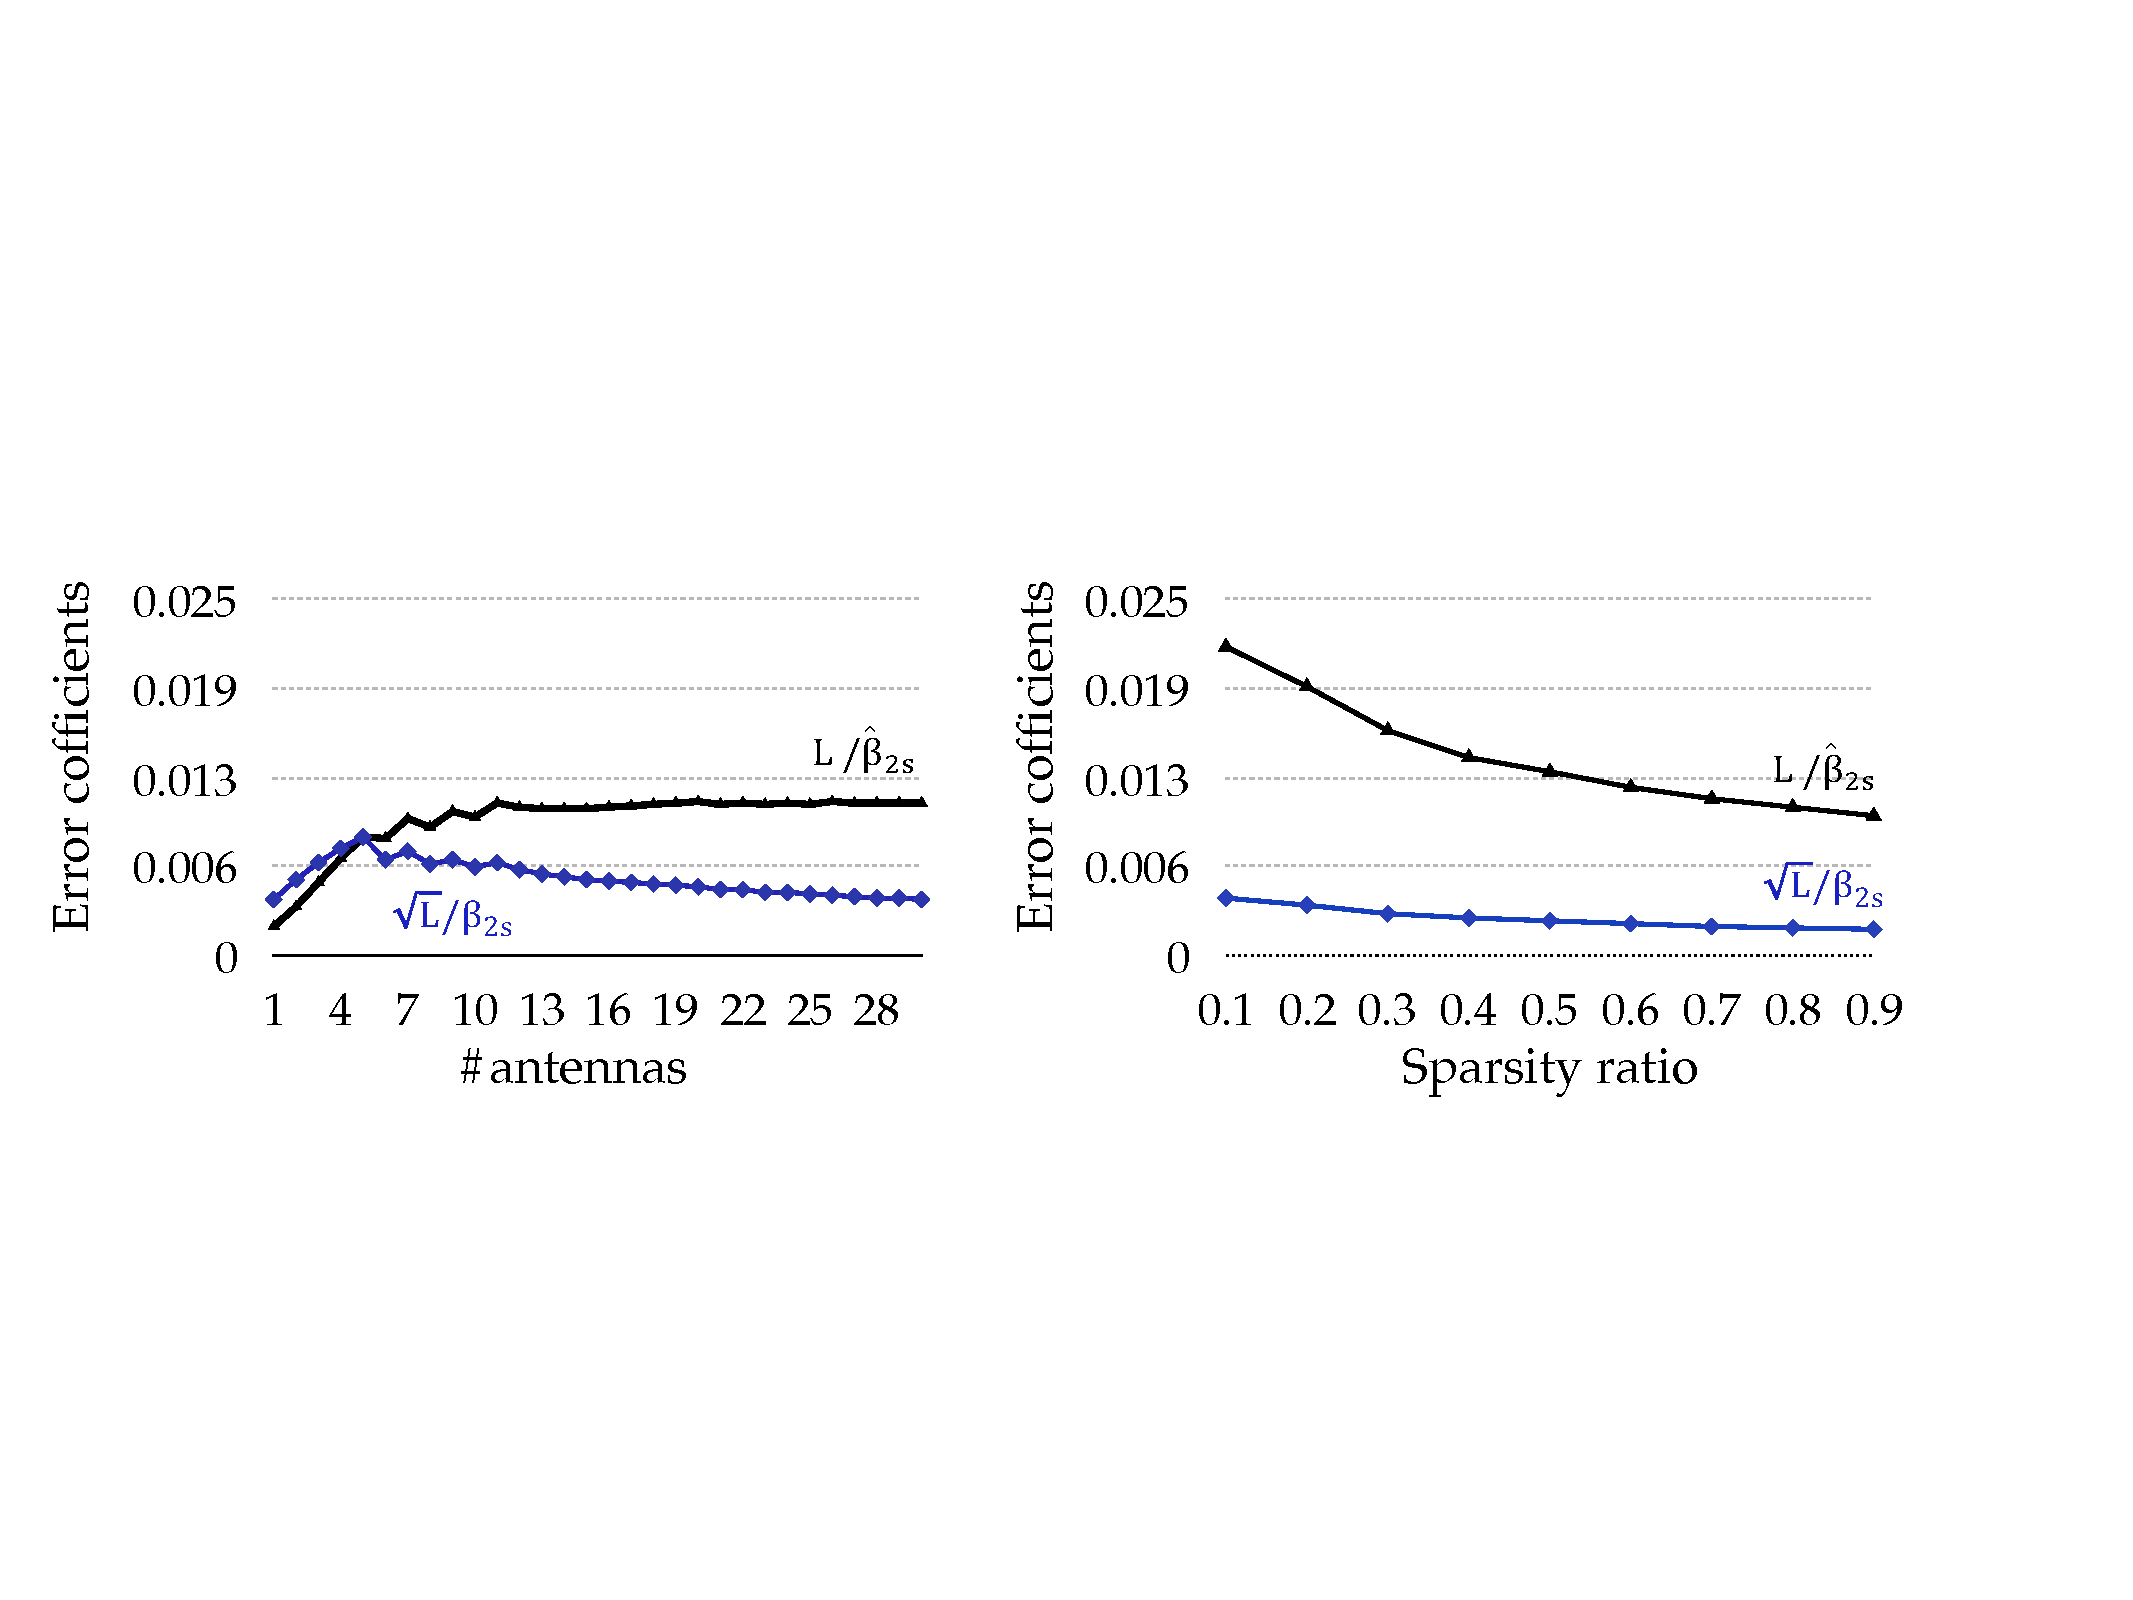
\includegraphics[width=0.85\columnwidth, angle=0]{figs/beta_k.pdf}
\caption{Monitoring the error coefficients: $\sqrt{L}/\beta_{2s}$ and $L/\hat{\beta}_{2s}$ that scale $ \sigma_n$ and $\|{\bf x}^s \|_2$ that appear in the recovery error bound, respectively. Sparsity ratio stands for $s/M$. The numerical value of coefficients guarantees that $\|{\bf x}^{[n+1]}-{\bf x}^s\|_2/\|{\bf x}^s \|_2$ is sufficiently small regardless of the number of bits to represent ${\bf \Phi}$.}
\label{fig:beta}
\end{figure}
%\vspace{-.1em}
\vspace{0.5em}

In Fig.~\ref{fig:beta}, for station CS302 of LOFAR, we first form the image grid and compute and adjust ${\bf \Phi}, \hat{\bf \Phi}$ such that $\alpha_{2s}, \hat{\alpha}_{2s}\leq 1/16$ holds. We refer the reader to the supplementary material for more details. Then we numerically compute the scaling factors of errors $\sigma_n$ and ${\epsilon}_{\textrm sky}$: $\sqrt{L}/\beta_{2s}$ and ${L}/{\hat{\beta}_{2s}}$, respectively. Theorem~\ref{main_theorem_TH} states that the recovery error is induced by two terms: $\sqrt{L}/\beta_{2s}$ and $L/{\hat{\beta}_{2s}$. Therefore, we investigate these scaling over various antenna numbers and sparsity level. The results suggest that 2-bits IHT has a negligible quantization error when applied radio interferometry imaging problem.

%\vspace{-1em}
\subsection{FPGA Implementation Details} \label{sec:fpga}
%\vspace{-0.5em}

Field-Programmable Gate Arrays (FPGA) are an alternative to commonly used Graphics Processing Units (GPU) for accelerated processing of compute intensive machine learning workloads. The custom logic fabric of an FPGA enables the design of specialized compute units, which is very advantageous when working on extremely low-precision and irregular numeric formats, such as 2 bit numbers. Thanks to the microarchitectural flexibility advantage, it is possible to achieve near linear speed-up when lowering the precision of data that is read from the memory. This has been shown recently for stochastic gradient descent (SGD) when training linear models~\citep{zhang2017zipml, kara2017fpga}. In this work, we use the open-source FPGA implementation from the mentioned works and modify it to perform IHT.
\vspace{0.5em}

In terms of the computation, we need to modify two parts of the design to convert it from performing SGD to IHT: 1) Instead of updating the model after a mini-batch count is reached, we update it after all samples are processed and the true gradient is available. 2) After each epoch, we perform a binary search on the updated model to find the threshold value satisfying that only top $S$ values are larger than the  threshold.

\begin{figure}[t!]
\centering
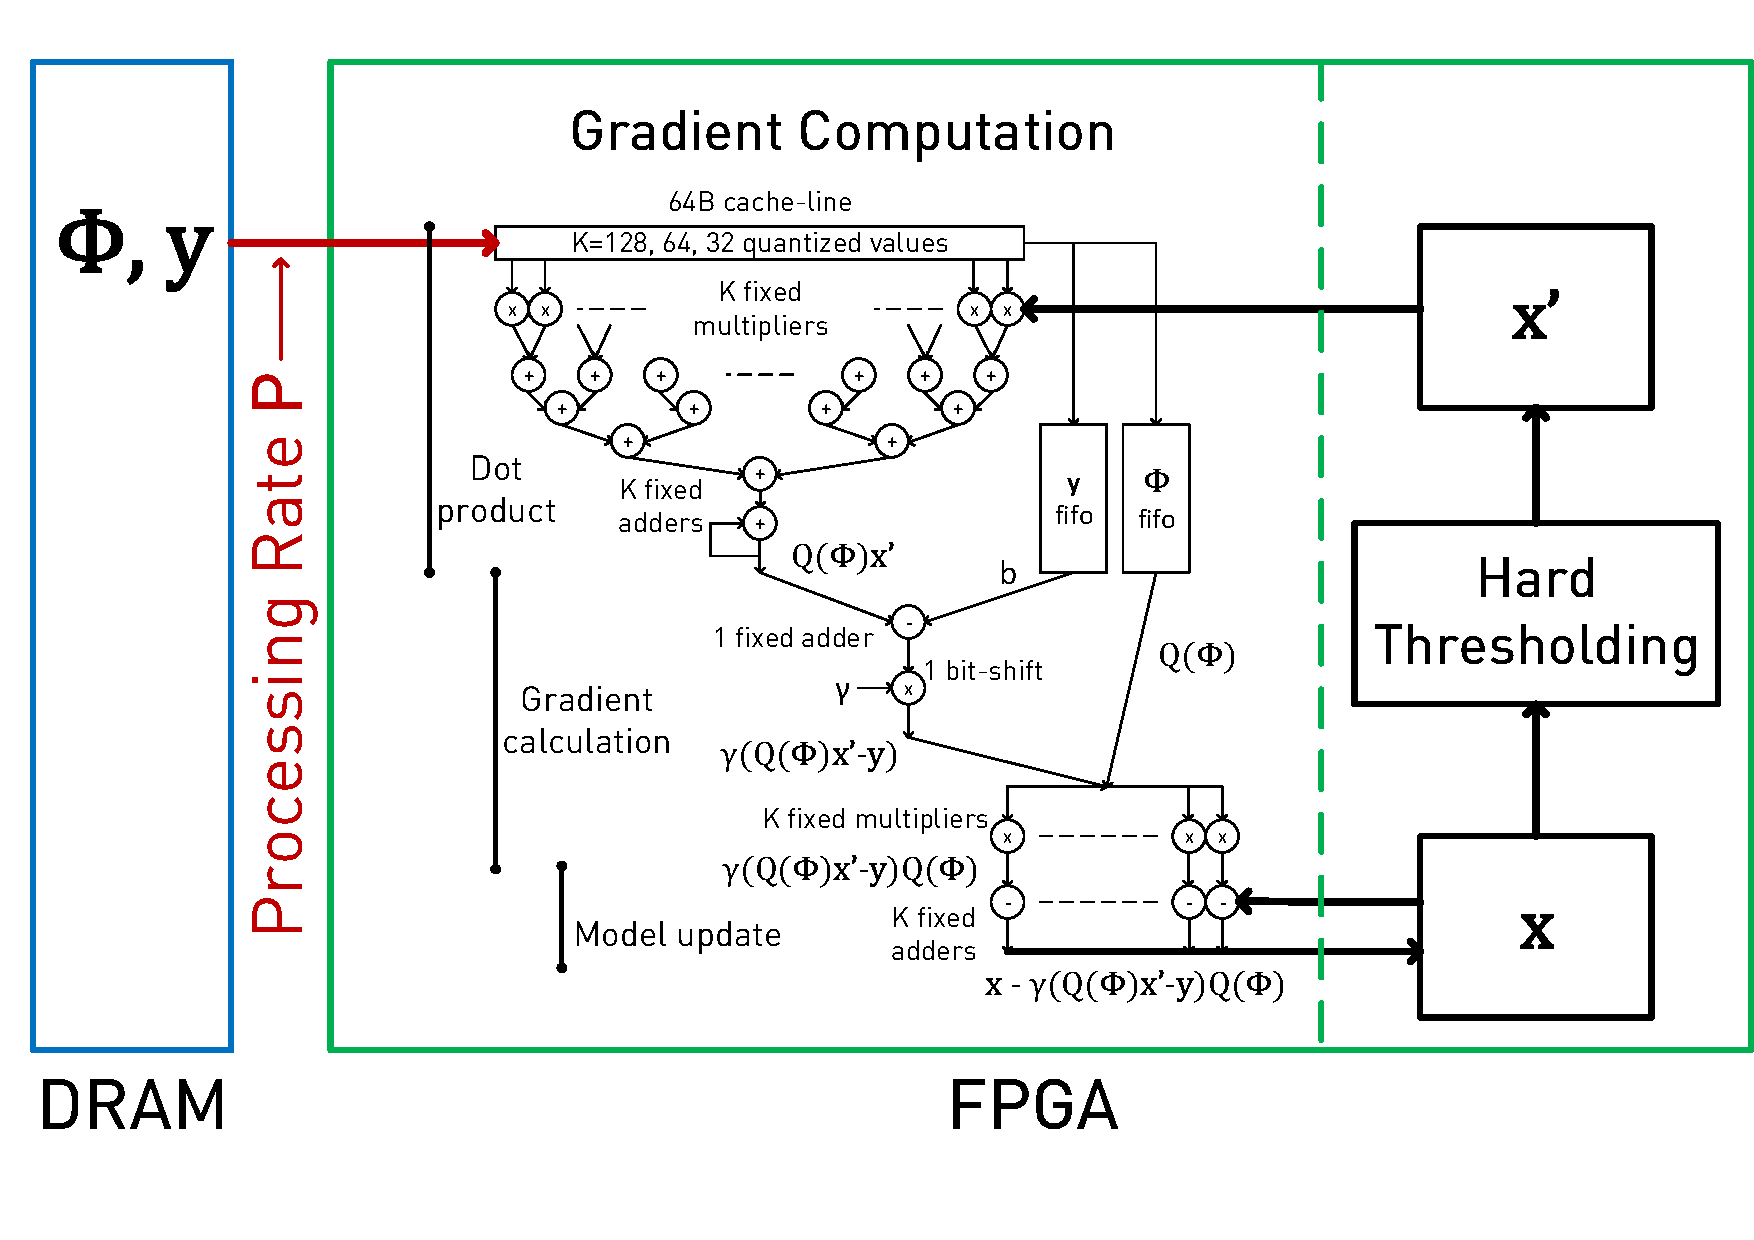
\includegraphics[width=0.75\textwidth, angle=0]{figs/niht_fpga.pdf}
\caption{IHT on an FPGA-based system.}
\label{fig:fpga}
\end{figure}

\vspace{0.5em}
{\bf Performance analysis} The gradient computation unit as shown in Fig.~\ref{fig:fpga} reads the measurement matrix ${\bf \Phi}$ and the measurements ${\bf y}$ from main memory and keeps ${\bf x}$ in on-chip memory. 
We note that transferring ${\bf \Phi}$ from main memory will be necessary in most practical settings, where the matrix ${\bf \Phi}$ is too large to fit onto the FPGA. 
The FPGA is able to process data from memory at a rate of ${\bf P}=12.8\,GB/s$. 
Thus, performance will be bound on this rate ${\bf P}$ for processing ${\bf \Phi}$ and ${\bf y}$, which becomes the system bottleneck. The time for each iteration is given by 
$T = size({\bf \Phi})/{\bf P}$, since $size({\bf y}) \ll size({\bf \Phi})$. 
We can achieve significant speed-up by quantizing ${\bf \Phi}$, simply because we reduce the amount of data to be transferred: more entries arrive with each transfer from main memory. 
%, because the time for each epoch is given by
%$T = size({\bf \Phi})/{\bf P}$, since $size({\bf y}) \ll size({\bf \Phi})$. The essential idea behind achieving %linear speed-up is keeping ${\bf P}$ constant as the precision of ${\bf \Phi}$ is lowered (${\bf P}\to \land \, %size({\bf \Phi})\downarrow$), which leads to more values arriving within each transfer from main memory. 
The processing rate ${\bf P}$ can be kept constant on an FPGA, because we can adapt the gradient computation unit's microarchitecture and increase its internal parallelism to handle more values per incoming line. 
\vspace{0.5em}

{\bf Computing ${\bf \Phi}$ on the fly} The above analysis focuses on the case when ${\bf \Phi}$ 
is stored in main memory, in which case quantization helps to reduce the amount of 
data transferred between the main memory and FPGA. In some applications, ${\bf \Phi}$
can be calculated on the fly, inside the FPGA. Also in this case, quantization can help 
achieve better performance.
The reason why quantizing ${\bf \Phi}$ helps, even if it can be calculated on the fly, is
that a quantized ${\bf \Phi}$ saves many crucial resources (e.g., multipliers) that
are limited on an FPGA. These resource savings are very important in achieving a higher 
internal parallelism, for instance, to speed up the computation of ${\bf \Phi}\times{\bf x}$. 
For example, it has been shown by~\citep{kara2017fpga} that to go from a 64-value dot product to 128-value
dot product on an FPGA, it is necessary to lower the precision of one side of the dot product to 2-bits.

%\vspace{-1em}
\section{Experimental Results}\label{section_experiments}
%\vspace{-0.5em}

We assess the empirical performance of our approach using the radio interferometer measurements from a real telescope: the LOw Frequency ARray (LOFAR). We first demonstrate that the accuracy achieved in the low precision setting is comparable with high precision IHT and other state-of-art methods; we then show the speed-up on FPGA.

%\vspace{-1em}
\subsection{Accuracy of Sky Recovery}
%\vspace{-0.5em}
We recover the full sky image of the resolution $256\times 256$ pixels (${\bf x} \in \mathbb{R}^{65,536}$ in vectorized form) by employing 30 low-band antennas of LOFAR CS302 station that operates in 15-80 MHz frequency band where the sky is populated with 30 strong sources, that is, ${\bf y} \in \mathbb{C}^{900}$, $\hat{\bf \Phi} \in \mathbb{C}^{900\times 65,536}$. The signal-to-noise ratio is 0 dB at the antenna level, i.e., $10\log_{10}(\|{\bf \Phi x}\|_2^2/\|{\bf e}\|_2^2) = 0$ dB. 
\vspace{0.5em}

%\vspace{-0.5em}
{\bf Improving least square estimates}
Fig.~\ref{fig:sky_images} provides an example of sky recoveries: (a) ground truth estimated over 12 hours of observation, (b) a least square estimate of underlying sky (or dirty image in the nomenclature of radio astronomy), (c) 32 bit and (d) 2\&8 bit (normalized) IHT which uses 2 bits for the measurement matrix and 8 bits for the observation. This experiment indicates that low precision IHT captures the sky sources successfully even when only 2 bit are used to compress ${\bf \Phi}$. Thus, we can drastically reduce the data precision yet still estimate the sky precisely.
%\vspace{-.1em}
\vspace{0.5em}

This strong empirical performance is not completely surprising. Mathematically, the measurement matrix we formed here reflects the phase relations, as induced by the antenna locations.  That is, each time a bit $r_{m, n}$ or $c_{m, n}$ flips its sign where $\hat{\bf \Phi}_{m, n} = r_{m, n} +j c_{m,n}$, $m = {1, 2, ..., M}$ and $n = {1, 2, ..., N}$, we approximately know the change in horizontal and vertical directions on the ground, preserving the phase information required for interferometric imaging even at very low precision.
\vspace{0.5em}

%Recall from the former discussions that noise in receivers is far stronger than the weak incoming signals thus low SNR at the antenna level results, i.e., usually ranged from -5 to 5 dB. The CLEAN algorithm notably underperforms in the presence of significant noise. This undesirable property is yet not surprising. A careful look into the the algorithmic steps, it apparently matches also to the noise artefacts in the image considering them as a point source. This can also be justified mathematically: we designed the problem such that an execution of {CLEAN} corresponds to the first iteration recovery of IHT, which interprets our numerical results. 

%The reader might argue that, besides being on its most possible realistic setting, the above experiment does not fully capture the performance of low precision iht especially when only 2-bits are used to represent a dense measurement matrix. 
\vspace{0.5em}

%\vspace{-0.3em}
{\bf Comparison to state-of-art methods}
We compare low precision IHT to full precision IHT, CoSaMP and an $\ell_1$-based approach in terms of their capability to recover sparse signals. For this particular formulation of the interferometric imaging problem, they can iteratively build up an estimate of the sky map ${\bf x}$. To avoid bias towards any algorithm, we optimized each algorithm independently.

\begin{figure}[t]
\centering
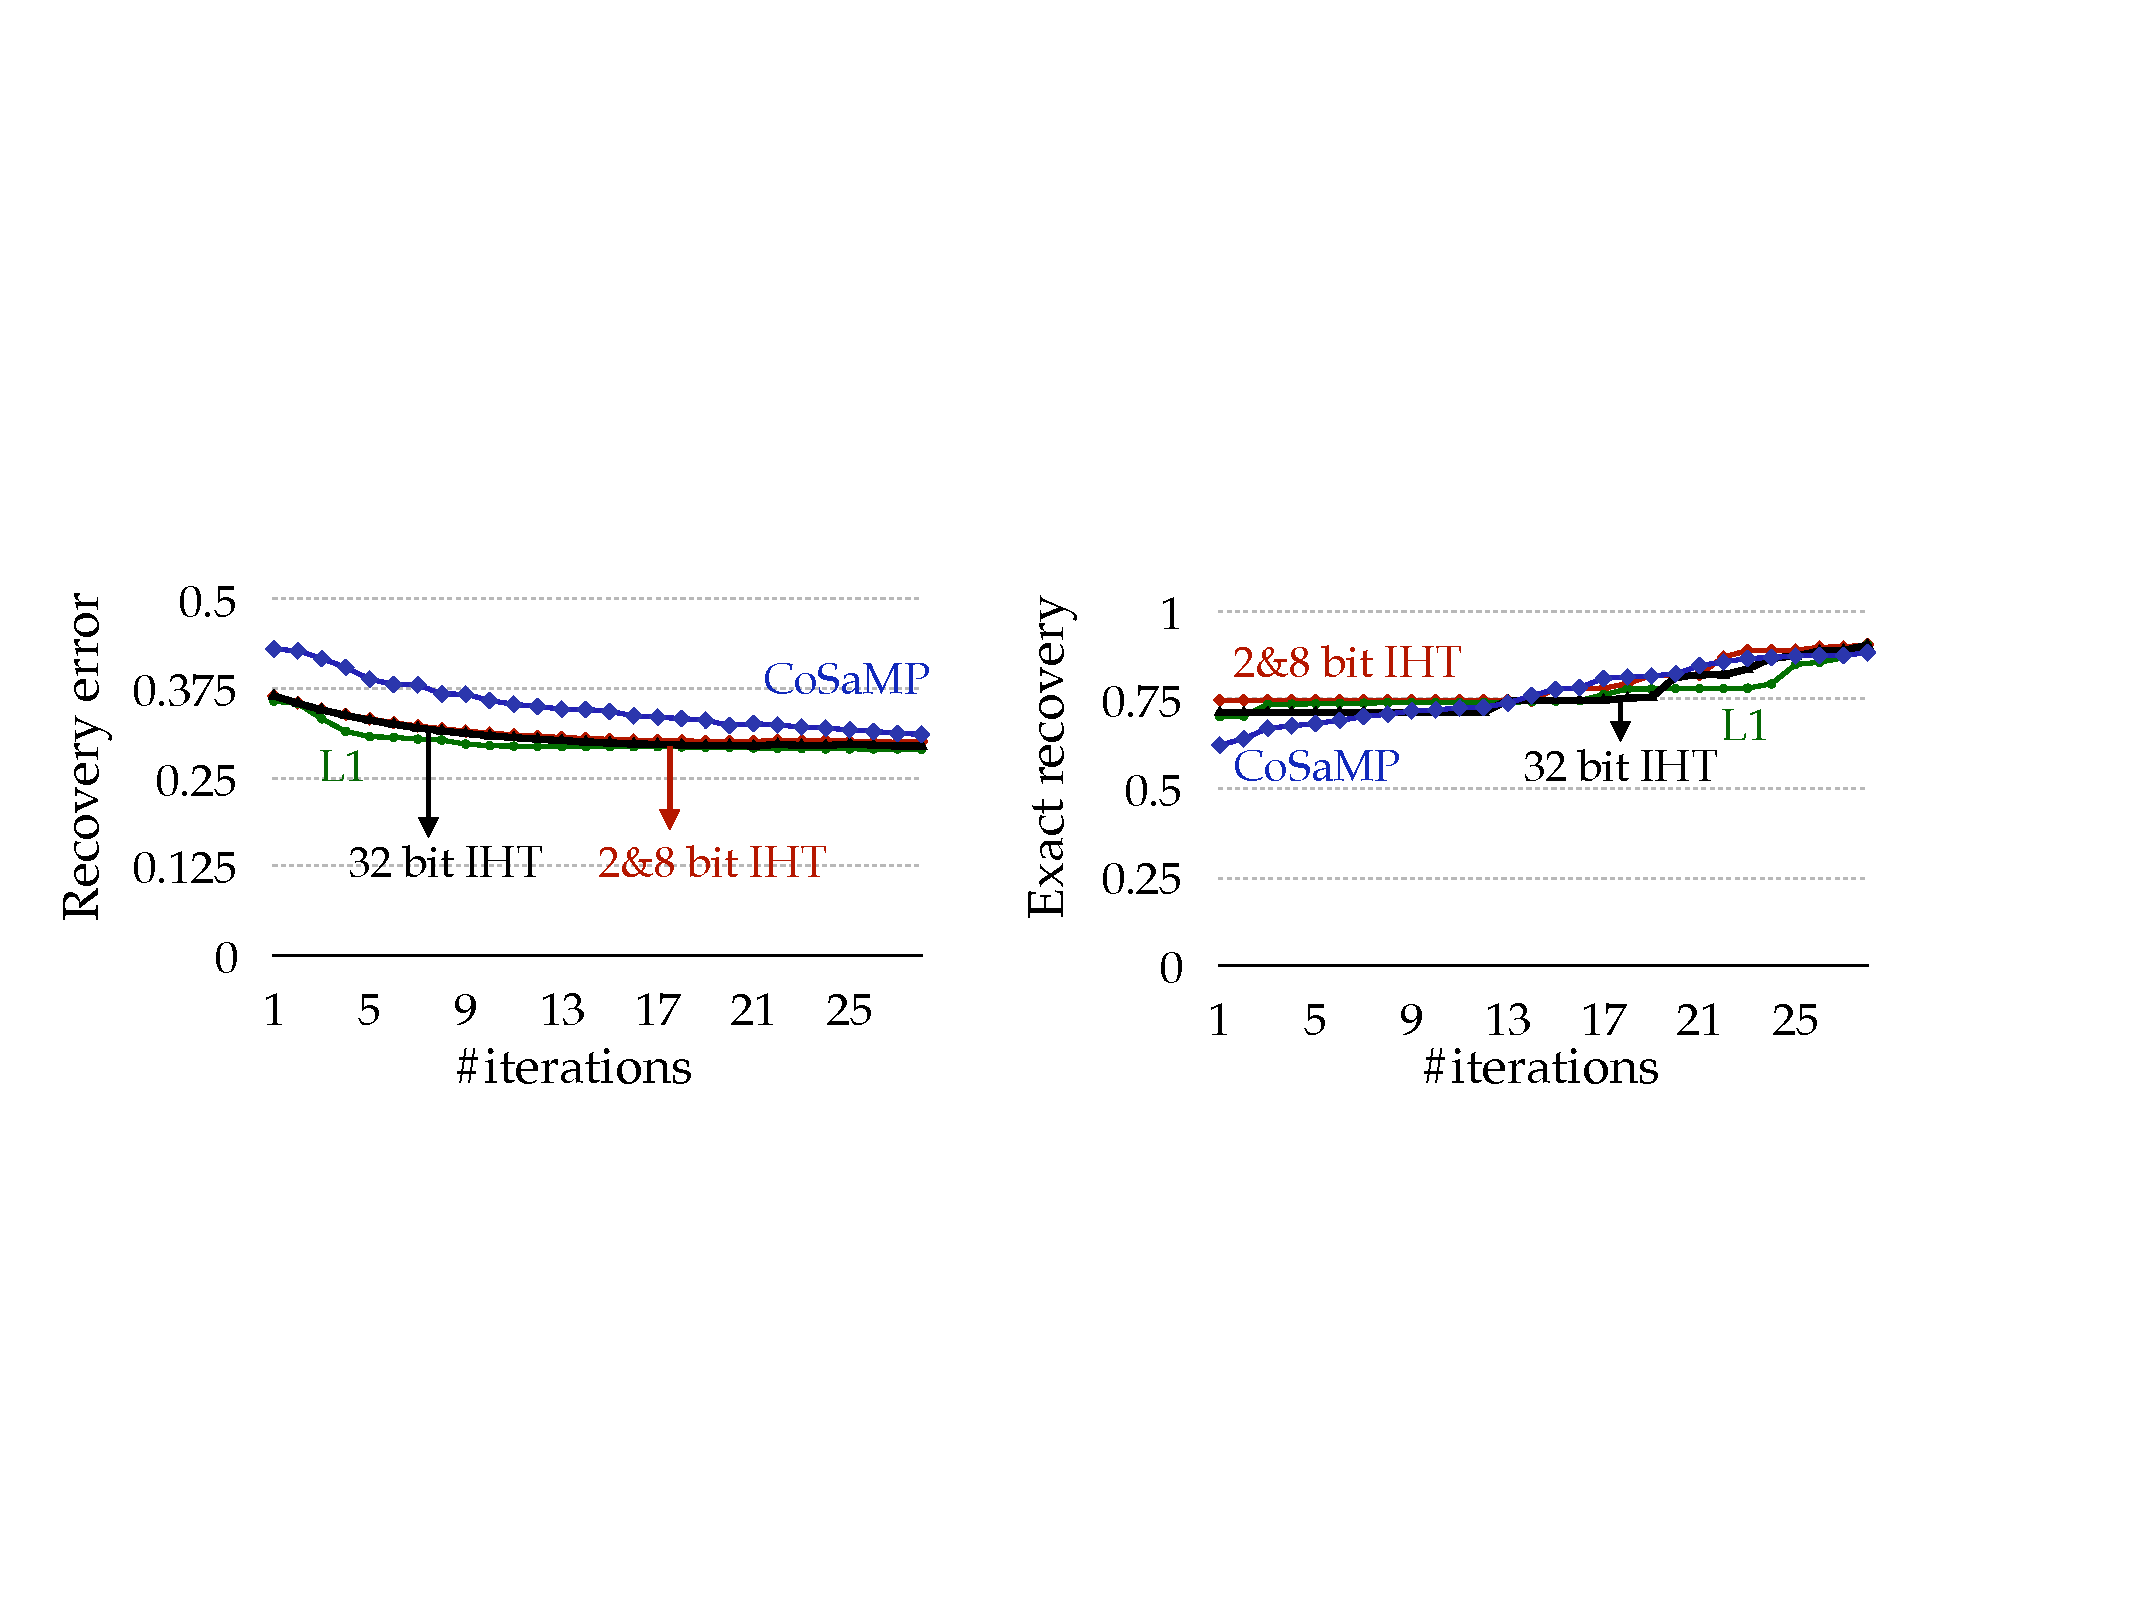
\includegraphics[width=0.85\columnwidth, angle=0]{figs/comparison_k.pdf}
\caption{Comparison of recovery error and exact recovery (support): {2\&8 bit} IHT vs. 32 bit IHT, CoSaMP, \& $\ell_1$.}
\label{fig:comparison}
\vspace{-1em}
\end{figure}
\vspace{0.5em}

We first evaluate algorithms through two metrics: (1) the recovery error and (2) exact recovery, that is, the ratio of support that is successfully recovered. In radio interferometry, however, it is customary to use number of true celestial sources resolved in the recovered image as a performance metric, i.e., true-positive findings. That is, the performance of the algorithms is no longer described by its ability to recover support entirely but the sky objects, which possess higher error tolerance. 
We demonstrate in Fig.~\ref{fig:comparison} that IHT performs as well as its alternatives and compatible to $\ell_1$-minimization in terms of its exact recovery performance. Empirical results suggest that the celestial sources can still be recovered when dramatically quantizing ${\bf \Phi}$.
%\vspace{-.2em}


\vspace{0.5em}
{\bf Discussion:} This experiment is informative merely on the accuracy of the results obtained implementing these alternative algorithms. A fair comparison involves the analysis of different properties such as speed and storage requirements, flexibility and ease of implementation. 
%CoSaMP has strong theoretical guarantee when the least squares solution is supplied and requires the solution to an inverse problem at each iteration, which is costly in general and demands better storage capability~\citep{needel2008cosamp}. On the other hand, 
IHT is known to outperform CoSaMP when ${\bf \Phi}$ has similar entries in magnitude~\citep{blumensath2012greedy}, which is confirmed by our experiments. Empirical evidence further suggests that IHT performs nearly as well as the $\ell_1$-based approach. %Referring back to supplemetary material, the CLEAN requires a 2D Fourier inversion and deconvolution per iteration thus the operational expense of the method is relatively higher compared to those of IHT and CoSaMP~\citep{simeoni2015rai}. 
The low precision approach has similar recovery performance as high precision IHT, as shown
in Fig.~\ref{fig:comparison}.


% \., which is vastly superior to the resitual in...
% This suggest we can drastically reduce bidi bidi
% Such a result has potentially profound consequences for the power consumption.

%\vspace{-1em}
\subsection{Speed-up on FPGA}
%\vspace{-0.5em}

We demonstrate the speed up for performing IHT on the FPGA-based system in Fig.~\ref{fig:fpga_time}. For the time spent per iteration, we see that quantization, and the resulting compression of the measurement matrix ${\bf \Phi}$ leads to near linear speed up for recovering the support vector. As previously studied in the performance analysis part in Section~\ref{sec:fpga}, all variants (full precision to lowest precision) of IHT on FPGA can consume ${\bf \Phi}$ at the same rate, and therefore the runtime of IHT depends linearly on the size of ${\bf \Phi}$, leading to linear speed ups that we observe in the experiments.
\vspace{0.5em}

In terms of end-to-end performance, we measure the time for
each precision level needs to reach support recovery
ratio 90\% and calculate the speedup. The 2\&8-bit IHT variant reaches the same support recovery
ratio 9.19$\times$ faster.


%A subtle observation related to the particular system's characteristics: When comparing the runtime between 32-bit floating-point precision and 2-bit precision, we observe 7.7x speed up, although the data compression rate is 8x. The reason for that is, when using quantized ${\bf \Phi}$, the FPGA reads for each epoch a freshly quantized ${\bf \Phi}$ (due to stochastic quantization) and therefore reads from a different location in main memory; whereas when using full-precision ${\bf \Phi}$, the FPGA always reads from the same location in main memory, utilizing the cache more efficiently. This is the reason, why the speed up rate is not perfectly matching the compression rate.



\vspace{-1em}
\section{Discussion}\label{section_discussion}
%\vspace{-.5em}
We investigated the applicability of low precision schemes to sparse signal recovery problems, and introduced a low-precision NIHT variant, with theoretical guarantees and good practical performance, both in terms of accuracy and recovery time. 
The radio astronomy application validated our claims, and showed that the heuristic and rigorous arguments are in agreement with experiments. The results bear out that our approach offers similar accuracy with the high precision IHT even with far less precision of data points. Further, we showed that even when using 2 bits to represent data,  the accuracy of sparse approximations can still be preserved, and significant practical speed up can be achieved.
\vspace{0.5em}

There are several questions for future work. In particular: Can we devise algorithms which work with end-to-end low precision data representation? Can we extend these techniques to other greedy recovery algorithms, and other sparse recovery frameworks?
\begin{figure}[t!]
\centering
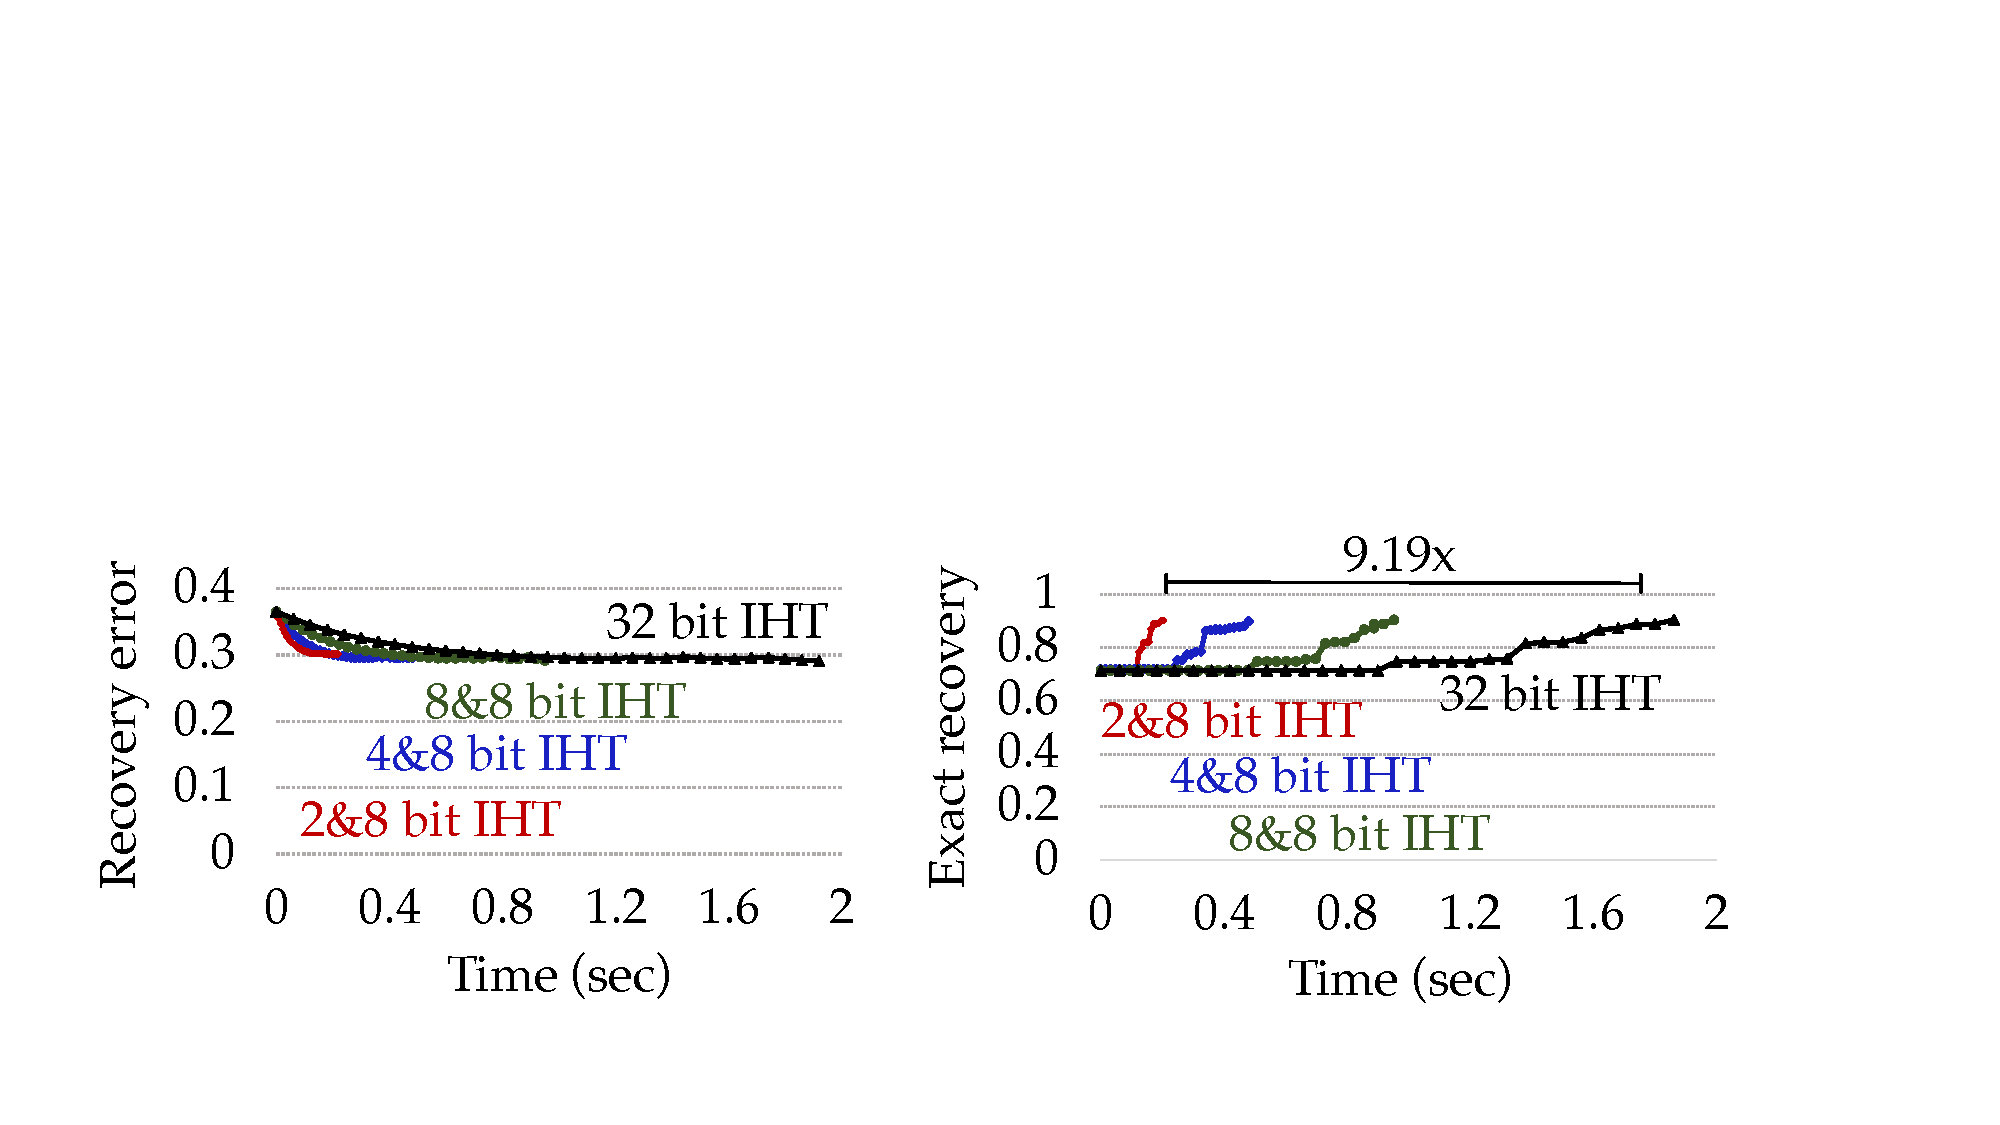
\includegraphics[width=0.8\columnwidth, angle=0]{figs/fpga_k.pdf}
\caption{Speed-up of low precision IHT on FPGA. 2\&8 bit IHT provides 9.19$\times$ speedup versus full-precision.}
\label{fig:fpga_time}
\end{figure}
\section*{Proofs}
We begin by introducing our notation.
\begin{enumerate}
    \item ${\bf y} = {\bf \Phi} {\bf x} + {\bf e} = {\bf \Phi} {\bf x}^s + {\bf \Phi}({\bf x}-{\bf x}^s) + {\bf e}$,
    \item $\boldsymbol{\varepsilon} = {\bf \Phi}({\bf x}-{\bf x}^s) + {\bf e}$, hence ${\bf y} = {\bf \Phi} {\bf x}^s + \boldsymbol{\varepsilon}$,
    \item $\boldsymbol{\epsilon_y} = Q({\bf y},b) - {\bf y}$,
    \item $\Gamma^{[n]} = \rm{supp}\{{\bf x}^{[n]} \}$, $\hat{\Gamma}^{[n]} = \rm{supp}\{\hat{{\bf x}}^{[n]} \}$ and $\Gamma^{s} = \rm{supp}\{{\bf x}^{s} \}$,
    \item $B^{[n]} = \Gamma^{[n]} \cup \Gamma^{s}$ and $B^{[n]} = \hat{\Gamma}^{[n]} \cup \Gamma^{s}$,
    \item ${\bf a}^{[n+1]} = \hat{{\bf x}}^{[n]} + \mu^{[n]}{\bf \Phi}^{\dag}({\bf y} - {\bf \Phi}\hat{{\bf x}}^{[n]})$ and $\hat{{\bf a}}^{[n+1]} = \hat{{\bf x}}^{[n]} + \hat{\mu}^{[n]}Q_{1}({\bf \Phi})^{\dag}({\bf y} - Q_2({\bf \Phi})\hat{{\bf x}}^{[n]})$,
    \item ${\bf x}^{[n+1]} = H_s({\bf a}^{[n+1]})$ and $\hat{{\bf x}}^{[n+1]} = H_s(\hat{{\bf a}}^{[n+1]})$,
    \item ${\bf r}^{[n]} = \hat{{\bf x}}^{[n]}-{\bf x}^s$.
\end{enumerate}
Assume $\mathbf{\bf \Phi}$ satisfies the non-symmetric Restricted Isometry Property 
\begin{equation}\label{rip}
\alpha_{s} \leq \frac{\|{\bf {\bf \Phi}} {\bf x}\|_2}{\|{\bf x}\|_2} \leq \beta_{s}
\end{equation}
for all ${\bf x}: \|{\bf x}\|_0 \leq s$, where $\alpha_s\in \mathbb{R}$ and $\beta_s \in \mathbb{R}$ are the lowest and largest singular value of ${\bf \Phi}$ such that $0<\alpha_s\leq \beta_s$, the so-called restricted isometric constants. Inherent from its definition, the restricted isometry holds for the quantized measurement matrix denoted by $Q({\bf {\bf \Phi}}, b_m)$ such that
\begin{equation}\label{rip_lowprecision}
\hat{\alpha}_{s} \leq \frac{\|Q({\bf {\bf \Phi}}, b_m) {\bf x}\|_2}{\|{\bf x}\|_2} \leq \hat{\beta}_{s}
\end{equation}
where $\hat{\alpha}_{s}$ and $\hat{\beta}_{s}$ are associated restricted isometry constants. For simplicity, we drop $b_m$, and use $Q({\bf {\bf \Phi}})$ instead. Also, let $\gamma_s=\beta_s/\alpha_s-1$ and $\hat{\gamma}_s=\hat{\beta}_s/\hat{\alpha}_s-1$.

\begin{remark}
The adaptive setting of step size parameter $\mu^{[n]}$ and $\hat{\mu}^{[n]}$ in normalized IHT is shown to satisfy
\begin{equation}\label{bounds_mu}
   1/\beta^2_{2s} \leq \mu^{[n]} \leq 1/\alpha^2_{2s},
\end{equation}
\begin{equation}\label{bounds_muhat}
   1/\hat{\beta}^2_{2s} \leq \hat{\mu}^{[n]} \leq 1/\hat{\alpha}^2_{2s}.
\end{equation}
\end{remark}


We will start by stating the following fundamental results.
\begin{lemma}\label{lemmas_on_phi}
{\rm{\citep{blumensath2010niht}}}
If ${\bf {\bf \Phi}}$ satisfies the restricted isometry property, then for $|\Gamma|\leq 2s$
\begin{equation}\label{mu*phi}
    \| {\bf {\bf \Phi}}_{\Gamma}^T{\bf x}\|_2 \leq \beta_{2s}\|{\bf x} \|_2,
\end{equation}
\begin{equation}\label{mu*phi*phi}
    \| \mu^{[n]}{\bf {\bf \Phi}}_{\Gamma}^T{\bf {\bf \Phi}}_{\Gamma}{\bf x}_{\Gamma}\|_2 \leq (\gamma_{2s}+1)\|{\bf x}_{\Gamma} \|_2,
\end{equation}
\begin{equation}\label{1-mu*phi*phi}
    \| ( {\bf I}- \mu^{[n]}{\bf {\bf \Phi}}_{\Gamma}^T{\bf {\bf \Phi}}_{\Gamma}){\bf x}_{\Gamma}\|_2 \leq \gamma_{2s}\|{\bf x}_{\Gamma} \|_2,
\end{equation}
\begin{equation}\label{mu*phi1*phi2}
     \| \mu^{[n]}{\bf {\bf \Phi}}_{\Upsilon}^T{\bf {\bf \Phi}}_{\Lambda}{\bf x}_{\Lambda}\|_2 \leq \gamma_{2s}\|{\bf x}_{\Lambda} \|_2,
\end{equation}
where $\Upsilon$ and $\Lambda$ are two disjoint sets (i.e., $\Upsilon \cap \Lambda = \emptyset$) such that $|\Upsilon \cup \Lambda| \leq 2s$. 
\end{lemma}
Clearly, similar results hold for $Q(\boldsymbol{{\bf \Phi}})$ such that
\begin{equation}\label{q_mu*phi}
     \|Q({\bf {\bf \Phi}})_{\Gamma}^T{\bf x}\|_2 \leq \hat{\beta}_{2s}\|{\bf x} \|_2,
\end{equation}
\begin{equation}\label{q_mu*phi*phi}
    \| \mu^{[n]}Q({\bf {\bf \Phi}})_{\Gamma}^TQ({\bf {\bf \Phi}})_{\Gamma}{\bf x}_{\Gamma}\|_2 \leq (\hat{\gamma}_{2s}+1)\|{\bf x}_{\Gamma} \|_2,
\end{equation}
\begin{equation}\label{1-q_mu*phi*phi}
    \| ( {\bf I}- \mu^{[n]}Q({\bf {\bf \Phi}})_{\Gamma}^TQ({\bf {\bf \Phi}})_{\Gamma}){\bf x}_{\Gamma}\|_2 \leq \hat{\gamma}_{2s}\|{\bf x}_{\Gamma} \|_2,
\end{equation}
\begin{equation}\label{q_mu*phi1*phi2}
    \| \mu^{[n]}Q({\bf {\bf \Phi}})_{\Upsilon}^TQ({\bf {\bf \Phi}})_{\Lambda}{\bf x}_{\Lambda}\|_2 \leq \hat{\gamma}_{2s}\|{\bf x}_{\Lambda} \|_2.
\end{equation}

\begin{lemma} \label{residual_lemma}
{\rm{\citep{blumensath2010niht}}}
For any ${\bf x}$, let ${\bf x}^s$ be the best s-term approximation to ${\bf x}$ and $\Upsilon$ be a set with at most s elements. Then
\begin{equation}\label{residual_x_bound}
\|\mu^{[n]}{\bf \Phi}^T_{\Upsilon} {\bf \Phi} ({\bf x}-{\bf x}^s)\|_2 \leq (1+\gamma_{2s})\big [\|{\bf x}-{\bf x}^s\|_2 ]+ \frac{\|{\bf x}-{\bf x}^s\|_2}{\sqrt{s}}\big].
\end{equation}
\end{lemma}
Based on the properties above, the restricted isometry, which we will require repeatedly throughout the proof, has several other consequences, summarized as follows.

\begin{corollary}\label{corollary_auxiliary_results}
Suppose $Q(\boldsymbol{{\bf \Phi}})$ satisfies restricted isometry property in Eqn. \ref{rip_lowprecision}. Then
\begin{equation}\label{mu_phi}
    \| ({\mu}^{[n]}{\bf {\bf \Phi}}_{\Gamma}^T-\hat{\mu}^{[n]}Q({\bf {\bf \Phi}})_{\Gamma}^T){\bf x}_{\Gamma}\|_2 \leq \rm{max}(({1+\gamma_{2s}})/{\beta_{2s}}-{1}/{\hat{\beta}_{2s}}, ({1+\hat{\gamma}_{2s}})/{\hat{\beta}_{2s}}-{1}/{\beta_{2s}})\| {\bf x}_{\Gamma}\|_2,
\end{equation} 
\begin{equation}\label{mu_phi2}
    \|( \mu^{[n]}{\bf \Phi}_{\Gamma}^T\boldsymbol{\Phi}_{\Gamma} - \mu^{[n]}Q_1(\boldsymbol{\Phi})_{\Gamma}^TQ_2(\boldsymbol{\Phi})_{\Gamma}){\bf x}_{\Gamma}\|_2 \leq \rm{max}(\gamma_{2s}, \hat{\gamma}_{2s})\| {\bf x}_{\Gamma}\|_2,
\end{equation}
\begin{equation}\label{mu_phi2_diff}
    \| (\mu^{[n]}\boldsymbol{\Phi}_{\Upsilon}^T\boldsymbol{\Phi}_{\Lambda} - \mu^{[n]}Q_1(\boldsymbol{\Phi})_{\Upsilon}^TQ_2(\boldsymbol{\Phi})_{\Lambda}){\bf x}_{\Lambda}\|_2 \leq \rm{max}(\gamma_{2s}, \hat{\gamma}_{2s})\| {\bf x}_{\Lambda}\|_2.
\end{equation}
\end{corollary}
\begin{proof}
As a simple consequence of restricted isometry property, the singular values of ${\bf \Phi}_{\Gamma}$ lie between $\alpha_{2s}$ and $\beta_{2s}$. Reminding that $\mu^{[n]}$ is chosen to satisfy $1/\beta^2_{2s}\leq \mu^{[n]}\leq 1/\alpha^2_{2s}$ we have
\begin{equation}
\begin{aligned}
   1/\beta_{2s} \| {\bf x}_{\Gamma}\|_2\leq \|{\mu}^{[n]}{\bf {\bf \Phi}}_{\Gamma} {\bf x}_{\Gamma}\|_2\leq (1+\gamma_{2s})/\beta_{2s}\| {\bf x}_{\Gamma}\|_2.
\end{aligned}
\end{equation}
\end{proof}
It similarly holds for $Q(\boldsymbol{{\bf \Phi}})$:
\begin{equation}
\begin{aligned}
   1/\hat{\beta}_{2s} \| {\bf x}_{\Gamma}\|_2\leq \|{\hat{\mu}}^{[n]}Q({\bf {\bf \Phi}})_{\Gamma} {\bf x}_{\Gamma}\|_2\leq (1+\hat{\gamma}_{2s})/\hat{\beta}_{2s}\| {\bf x}_{\Gamma}\|_2.
\end{aligned}
\end{equation}
Singular values of ${\mu}^{[n]}{\bf {\bf \Phi}}_{\Gamma}^T-\hat{\mu}^{[n]}Q({\bf {\bf \Phi}})_{\Gamma}^T$ therefore fall in the interval $[({1+\hat{\gamma}_{2s}})/{\hat{\beta}_{2s}}-{1}/{\beta_{2s}}$, $({1+\gamma_{2s}})/{\beta_{2s}}-{1}/{\hat{\beta}_{2s}}]$. Eqn. \ref{mu_phi} then trivially holds.
\vspace{0.5em}

Using restricted isometry property in Eqn. \ref{rip} \& \ref{rip_lowprecision} \  over 2s-sparse vectors, similar argument holds for Eqn. \ref{mu_phi2}, that is, the singular values of $\boldsymbol{\Phi}_{\Gamma}$ and $Q(\boldsymbol{\Phi})_{\Gamma}$ fall into $[1, 1+ \gamma_{2s}]$ and $[1, 1+ \hat{\gamma}_{2s}]$, respectively. Then $\|\mu^{[n]}\boldsymbol{\Phi}_{\Gamma}^T\boldsymbol{{\bf \Phi}}_{\Gamma} - \mu^{[n]}Q_1(\boldsymbol{\Phi})_{\Gamma}^TQ_2(\boldsymbol{\Phi})_{\Gamma}\|_2$ is bounded above by the term $\rm{max}((1+\hat{\gamma}_{2s})-1, (1+\gamma_{2s})-1)$, which proves Eqn. \ref{mu_phi2}. 
\vspace{0.5em}

Eqn. \ref{mu_phi2_diff} is a consequence of the fact that $-\mu^{[n]}\boldsymbol{{\bf \Phi}}_{\Upsilon}^T\boldsymbol{{\bf \Phi}}_{\Lambda}$ is a submatrix of $\rm{I}-\mu^{[n]}\boldsymbol{{\bf \Phi}}_{\Upsilon \cup \Lambda}^T\boldsymbol{{\bf \Phi}}_{\Upsilon \cup \Lambda}$, which in turn implies that $\|\mu^{[n]}\boldsymbol{{\bf \Phi}}_{\Upsilon}^T\boldsymbol{{\bf \Phi}}_{\Lambda}\|_2 \leq \|\rm{I}-\mu^{[n]}\boldsymbol{{\bf \Phi}}_{\Upsilon \cup \Lambda}^T\boldsymbol{{\bf \Phi}}_{\Upsilon \cup \Lambda} \|_2$, (i.e., spectral norm of a submatrix is bounded by the norm of its full matrix). Using Eqn. \ref{mu*phi*phi}, the eigenvalues of $\mu^{[n]}\boldsymbol{{\bf \Phi}}_{\Upsilon}^T\boldsymbol{{\bf \Phi}}_{\Lambda}$ can be shown to be in $[0, \gamma_{2s}]$, and in parallel, $\hat{\mu}^{[n]}Q(\boldsymbol{{\bf \Phi}})_{\Upsilon}^TQ(\boldsymbol{{\bf \Phi}})_{\Lambda}$ in $[0, \hat{\gamma}_{2s}]$. The difference $\rm{I}-\mu^{[n]}\boldsymbol{{\bf \Phi}}_{\Upsilon \cup \Lambda}^T\boldsymbol{{\bf \Phi}}_{\Upsilon \cup \Lambda}$ then have eigenvalues no larger than $\rm{max}(\gamma_{2s}, \hat{\gamma}_{2s})$.
\begin{lemma}\label{lemma_on_quantized_vector}
Let $Q(\cdot, b): \mathbb{R}^M\times \mathbb{Z}^+ \rightarrow \mathbb{R}^d$ denote quantization operator described in the paper. For any ${\bf v}\in \mathbb{R}^d$, the norm of quantization error can be bounded by
\begin{equation}\label{quantization_error}
    \mathbb{E}[\| Q({\bf v}, b) - \hat{\bf v}\|_2] \leq \frac{\sqrt{M}}{2^{b-1}}
\end{equation}
where $\hat{\bf v}$ is a scaled version of ${\bf v}$ so that every component is normalized to $[-1, 1]$.
\end{lemma}
\begin{remark}
For efficient fixed-point computation on Field Programmable Gate Array, we need an odd number of quantization levels, and therefore total number of levels for $b$ bit quantization is $2^{b-1}+1$. That is, the interval between two consecutive levels is $2^{b-1}$ provided the values are confined in the interval $[-1, 1]$ a priori.
\end{remark}
\begin{proof}
Using Jensen's inequality we can easily show that
\begin{equation}\label{quantization_error_bound1}
\begin{split}
    \mathbb{E}[\| Q(\hat{\bf v}, b) - \hat{\bf v}\|_2] &= \mathbb{E}\left[\sqrt{\| Q(\hat{\bf v}, b) - \hat{\bf v}\|^2_2} \right]\\
    &\leq \sqrt{\mathbb{E}[\| Q(\hat{\bf v}, b) - \hat{\bf v}\|^2_2]}\\
    &\leq \sqrt{\sum_{i=1}^{M} \mathbb{E}[\big (Q(\hat{\bf v}, b)_i -\hat{v_i}\big)^2]}\\
    &\leq \sqrt{\sum_{i=1}^{M} \mathbb{P}(Q(\hat{\bf v}, b)_i = \ell_j)(\hat{v}_i-\ell_j)^2 + \mathbb{P}(Q(\hat{\bf v}, b)_i = \ell_{j+1})(\ell_{j+1}-\hat{v}_i)^2}.
\end{split}
\end{equation}
Our quantization scheme uses a stochastic approach such that $\mathbb{P}(Q(\hat{\bf v}, b)_i = \ell_j)=\frac{\ell_{j+1}-\hat{v}_i}{\ell_{j+1}-\ell_{j}}$, and hence $\mathbb{P}(Q(\hat{\bf v}, b)_i = \ell_{j+1})=1-\frac{\ell_{j+1}-\hat{v}_i}{\ell_{j+1}-\ell_{j}}$. Substituting these into Eqn. \ref{quantization_error_bound1} we have
\begin{equation}\label{quantization_error_sub}
\begin{split}
    \mathbb{E}[\| Q(\hat{\bf v}, b) - \hat{\bf v}\|_2] \leq \sqrt{\sum_{i=1}^{n} (l_{j+1}-Q(\hat{\bf v}, b)_i)(Q(\hat{\bf v}, b)_i-\ell_j)}.
\end{split}
\end{equation}

It can easily be seen that $(l_{j+1}-Q(\hat{\bf v}, b)_i)(Q(\hat{\bf v}, b)_i-\ell_j)$ is maximized when $Q(\hat{\bf v}, b)_i) =  \frac{\ell_{j+1}-\ell_j}{2}$, moreover quantization function implies that $\ell_{j+1}-\ell_j = \frac{1-(-1)}{l} = \frac{1}{2^{b-2}}$


\begin{equation}\label{quantization_error}
\begin{split}
    \mathbb{E}[\| Q(\hat{\bf v}, b) - \hat{\bf v}\|_2] &\leq \sqrt{\sum_{i=1}^{M} \frac{(\ell_{j+1}-\ell_j)^2}{4}}\\
    &\leq \frac{\sqrt{M}(\ell_{j+1}-\ell_j)}{2}\\
    &\leq \frac{\sqrt{M}}{2^{b-1}}.
\end{split}
\end{equation}
\end{proof}
%\begin{corollary}
% Let ${\boldsymbol{\phi}} \in \mathbb{R}^{m\times n}$. Using Lemma \ref{lemma_on_quantized_vector}, the quantization error over matrices can be bounded by
% \begin{equation}\label{quantization_error_matrices}
% \begin{split}
%     \mathbb{E}[\|Q(\boldsymbol{\phi}, b) -\hat{\boldsymbol{\phi}}\|_2] \leq \frac{\sqrt{mn}}{2^{b-1}}.
%     \end{split}
% \end{equation}
% \end{corollary}
% \begin{proof}
% coming soon
%\end{proof}



\subsection*{Proof of Theorem 3}
The recovery error can be split into two parts by using triangle inequality
\begin{equation}\label{main_theorem}
\begin{split}
   \mathbb{E}[ \|\hat{{\bf x}}^{[n+1]} - {\bf x}^s \|_2 | \hat{{\bf x}}^{[n]}] &= \mathbb{E}[\|\hat{{\bf x}}_{B^{[n+1]}}^{[n+1]} - {\bf x}_{B^{[n+1]}}^s \|_2| \hat{{\bf x}}^{[n]}] \\
    &\leq \mathbb{E}[\|\hat{{\bf x}}_{B^{[n+1]}}^{[n+1]} - \hat{{\bf a}}_{B^{[n+1]}}^{[n+1]} \|_2| \hat{{\bf x}}^{[n]}] + \mathbb{E}[\|\hat{{\bf a}}_{B^{[n+1]}}^{[n+1]} - {\bf x}_{B^{[n+1]}}^s \|_2| \hat{{\bf x}}^{[n]}].
    \end{split}
\end{equation}
where the equality follows from that $\hat{{\bf x}}^{[n+1]} - {\bf x}^s$ is supported over the set $B^{[n+1]} = \hat{\Gamma}^{[n+1]} \cup \Gamma^s$.

Recall that $\hat{{\bf x}}_{B^{[n+1]}}^{[n+1]}$ is a better s-term approximation to $\hat{{\bf a}}_{B^{[n+1]}}^{[n+1]}$ than ${\bf x}_{B^{[n+1]}}^{s}$ \big(i.e., $\|\hat{{\bf x}}^{[n+1]} - \hat{{\bf a}}_{B^{[n+1]}}^{[n+1]} \|_2\leq \| \hat{{\bf a}}_{B^{[n+1]}}^{[n+1]} - {\bf x}^s \|_2$\big). Then 
\begin{equation}
    \mathbb{E}[\|\hat{{\bf x}}^{[n+1]} - {\bf x}^s \|_2| \hat{{\bf x}}^{[n]}] \leq 2\mathbb{E}[ \|\hat{{\bf a}}_{B^{[n+1]}}^{[n+1]} - {\bf x}_{B^{[n+1]}}^s \|_2 | \hat{{\bf x}}^{[n]}].
\end{equation}
Using triangle inequality, we further have
\begin{equation}\label{nonproof_bound_final}
    \mathbb{E}[\|\hat{{\bf x}}^{[n+1]} - {\bf x}^s \|_2| \hat{{\bf x}}^{[n]}]\leq 2 \big [\mathbb{E}[\|\hat{{\bf a}}_{B^{[n+1]}}^{[n+1]} - {{\bf a}}_{B^{[n+1]}}^{[n+1]} \|_2  + \|{{\bf a}}_{B^{[n+1]}}^{[n+1]} - {{\bf x}}_{B^{[n+1]}}^{s} \|_2 | \hat{{\bf x}}^{[n]}]\big ]
\end{equation}

We now continue with the analysis referring to two terms on the right hand side of Eqn. \ref{nonproof_bound_final} separately.\\

{(a)} Expanding $\hat{{\bf a}}_{B^{[n+1]}}^{[n+1]}$ and ${{\bf a}}_{B^{[n+1]}}^{[n+1]}$ we have
\begin{equation}\label{quantization_error_terms}
    \begin{split}
      &\mathbb{E}[  \|\hat{{\bf a}}_{B^{[n+1]}}^{[n+1]} - {{\bf a}}_{B^{[n+1]}}^{[n+1]} \|_2| \hat{{\bf x}}^{[n]}] \\
      &= \mathbb{E}[\|\hat{\mu}^{[n]}Q_1({\bf {\bf \Phi}})_{B^{[n+1]}}^T\big(Q_y({\bf y})-Q_2({\bf {\bf \Phi}})\hat{{\bf x}}^{[n]}\big) - {\mu}^{[n]}{\bf {\bf \Phi}}_{B^{[n+1]}}^T({\bf y}-{\bf {\bf \Phi}}\hat{{\bf x}}^{[n]}) \|_2| \hat{{\bf x}}^{[n]}]\\
        &=\mathbb{E}[\|\hat{\mu}^{[n]}Q_1({\bf {\bf \Phi}})_{B^{[n+1]}}^T\big({\bf {\bf \Phi}} {\bf x}^s +\boldsymbol{\varepsilon}+\boldsymbol{\epsilon}_y-Q_2({\bf {\bf \Phi}})\hat{{\bf x}}^{[n]}\big) - {\mu}^{[n]}{\bf {\bf \Phi}}_{B^{[n+1]}}^T({\bf {\bf \Phi}}{\bf x}^s +\boldsymbol{\varepsilon}-{\bf {\bf \Phi}}\hat{{\bf x}}^{[n]}) \|_2| \hat{{\bf x}}^{[n]}]\\
        &=\mathbb{E}[\|\hat{\mu}^{[n]}Q_1({\bf {\bf \Phi}})_{B^{[n+1]}}^T\big(-Q_2({\bf {\bf \Phi}}) {\bf r}^{[n]} +\boldsymbol{\varepsilon}+\boldsymbol{\epsilon}_y+({\bf {\bf \Phi}}-Q_2({\bf {\bf \Phi}})){\bf x}^{s}\big)+{\mu}^{[n]}{\bf {\bf \Phi}}_{B^{[n+1]}}^T({\bf {\bf \Phi}}{\bf r}^{[n]} -\boldsymbol{\varepsilon}) \|_2| \hat{{\bf x}}^{[n]}]\\
        &\leq \|\big(\mu^{[n]}{\bf {\bf \Phi}}_{B^{[n+1]}}^T{\bf {\bf \Phi}} - \hat{\mu}^{[n]}Q_1({\bf {\bf \Phi}})_{B^{[n+1]}}^T Q_2({\bf {\bf \Phi}})\big) {\bf r}^{[n]} \|_2\\
        &\ \ \ \ \  +\|\big(\mu^{[n]}{\bf {\bf \Phi}}_{B^{[n+1]}}^T - \hat{\mu}^{[n]}Q_1({\bf {\bf \Phi}})_{B^{[n+1]}}^T \big)\boldsymbol{\varepsilon} \|_2\\
     &\ \ \ \  \  +\mathbb{E}[\|\hat{\mu}^{[n]}Q_1({\bf {\bf \Phi}})_{B^{[n+1]}}^T\boldsymbol{\epsilon}_y \|_2]\\
     &\ \ \ \  \  +\mathbb{E}[\| \hat{\mu}^{[n]}Q_1({\bf \Phi})_{B^{[n+1]}}^T\big({\bf {\bf \Phi}}-Q_2({\bf {\bf \Phi}})\big){\bf x}^s \|_2].
    \end{split}
\end{equation} where we used the expansion ${{\bf r}}^{[n]} = \hat{{\bf x}}^{[n]}-{\bf x}^s$. We further derive the terms governing the above expression in (a.1), (a.2), (a.3) and (a.4). \\

(a.1) Since ${\bf r}^{[n]}$ is supported over $B^{[n]}$, we clearly have
\begin{equation}\label{first_term_q_bound}
    \begin{split}
     \|\big(\mu^{[n]}&{\bf {\bf \Phi}}_{B^{[n+1]}}^T{\bf {\bf \Phi}} - \hat{\mu}^{[n]}Q_1({\bf {\bf \Phi}})_{B^{[n+1]}}^T Q_2({\bf {\bf \Phi}})\big) {\bf r}^{[n]} \|_2\\ &\leq\|\big(\mu^{[n]}{\bf {\bf \Phi}}_{B^{[n+1]}}^T{\bf {\bf \Phi}}_{B^{[n+1]}} - \hat{\mu}^{[n]}Q_1({\bf {\bf \Phi}})_{B^{[n+1]}}^T Q_2({\bf {\bf \Phi}})_{B^{[n+1]}}\big) {\bf r}_{B^{[n+1]}}^{[n]}\|_2\\
     & \ \ \ \ \ + \|\big ( \mu^{[n]}{\bf {\bf \Phi}}_{B^{[n+1]}}^T{\bf {\bf \Phi}}_{B^{[n]}\backslash B^{[n+1]}}-\hat{\mu}^{[n]}Q_1({\bf {\bf \Phi}})_{B^{[n+1]}}^T Q_2({\bf {\bf \Phi}})_{B^{[n]}\backslash B^{[n+1]}}\big ) {\bf r}_{B^{[n]}\backslash B^{[n+1]}}^{[n]} \|_2.
    \end{split}
\end{equation}
Using Eqn. \ref{mu_phi2} we have
\begin{equation}\label{residual_bound}
\begin{split}
 \|\big(\mu^{[n]}{\bf {\bf \Phi}}_{B^{[n+1]}}^T{\bf {\bf \Phi}}_{B^{[n+1]}} - \hat{\mu}^{[n]}Q_1({\bf {\bf \Phi}})_{B^{[n+1]}}^T Q_2({\bf {\bf \Phi}})_{B^{[n+1]}}\big) {\bf r}_{B^{[n+1]}}^{[n]}\|_2 &\leq \rm{max}(\gamma_{2s}, \hat{\gamma}_{2s})\| {\bf r}_{B^{[n+1]}}^{[n]}\|_2.
 \end{split}
\end{equation}
Let now $B^{[n+1]}$ be split into two disjoint sets $\Gamma_1$ and $\Gamma_2$, where $\Gamma_1 \cap \Gamma_2 = \emptyset$ and $|\Gamma_1|, |\Gamma_2| \leq s$. We have by Eqn. \ref{mu_phi2_diff}
{
\begin{equation}\label{residual_full_precision}
    \begin{split}
\|\big ( \mu^{[n]}{\bf {\bf \Phi}}_{B^{[n+1]}}^T&{\bf \Phi}_{B^{[n]}\backslash B^{[n+1]}}- \hat{\mu}^{[n]}Q_1({\bf \Phi})_{B^{[n+1]}}^T Q_2({\bf \Phi})_{B^{[n]}\backslash B^{[n+1]}}\big ) {\bf r}_{B^{[n]}\backslash B^{[n+1]}}^{[n]} \|_2 \leq\\
&\bigg({\|\big ( \mu^{[n]}{\bf \Phi}_{\Gamma_1}^T{\bf \Phi}_{B^{[n]}\backslash B^{[n+1]}} -\hat{\mu}^{[n]}Q_1({\bf \Phi})_{\Gamma_1}^T Q_2({\bf \Phi})_{B^{[n]}\backslash B^{[n+1]}}\big ) {\bf r}_{B^{[n]}\backslash B^{[n+1]}}\|_2^2\\
&\ \ \ + \|\big ( \mu^{[n]}{\bf \Phi}_{\Gamma_2}^T{\bf \Phi}_{B^{[n]}\backslash B^{[n+1]}} - \hat{\mu}^{[n]}Q_1({\bf \Phi})_{\Gamma_2}^T Q_2({\bf \Phi})_{B^{[n]}\backslash B^{[n+1]}}\big ) {\bf r}_{B^{[n]}\backslash B^{[n+1]}}\|_2^2}\bigg)^{\frac{1}{2}}\\
&\ \ \ \ \ \ \ \ \ \ \ \ \ \ \ \ \ \ \ \ \ \ \ \ \ \ \ \ \ \ \ \ \ \ \ \ \ \ \ \ \ \ \ \ \ \ \ \ \  \ \ \leq \sqrt{2}\rm{max}(\gamma_{2s}, \hat{\gamma}_{2s})\| {\bf r}_{B^{[n]}\backslash B^{[n+1]}}\|_2.
    \end{split}
\end{equation}
}
Combining Eqn. \ref{residual_bound} \& \ref{residual_full_precision} 
\begin{equation}\label{first_term_main_theorem}
    \begin{split}
     \|\big(\mu^{[n]}{\bf \Phi}_{B^{[n+1]}}^T{\bf \Phi} &- \hat{\mu}^{[n]}Q_1({\bf \Phi})_{B^{[n+1]}}^T Q_2({\bf \Phi})\big) {\bf r}^{[n]} \|_2\\
     &= \rm{max}(\gamma_{2s}, \hat{\gamma}_{2s})\|{\bf r}_{B^{[n+1]}}^{[n]}\|_2 + \sqrt{2}\rm{max}(\gamma_{2s}, \hat{\gamma}_{2s})\|{\bf r}_{B^{[n]}\backslash B^{[n+1]}} \|_2\\
     &\leq \sqrt{2}\rm{max}(\|{\bf r}_{B^{[n+1]}}^{[n]}\|_2 + \|{\bf r}_{B^{[n]}\backslash B^{[n+1]}} \|_2)\\
     &\leq 2 \rm{max}(\gamma_{2s}, \hat{\gamma}_{2s})\|{\bf r}^{[n]} \|_2
    \end{split}
\end{equation}
where the last inequality follows from the fact that ${\bf r}_{B^{[n+1]}}^{[n]}$ and ${\bf r}_{B^{[n]}\backslash B^{[n+1]}}$ are orthogonal.\\

(a.2) Expanding the second term in Eqn. \ref{quantization_error_terms}
\begin{equation}
    \begin{split}
        &\|(\mu^{[n]}{\bf \Phi}_{B^{[n+1]}} - \hat{\mu}^{[n]}Q_1({\bf \Phi})_{B^{[n+1]}}^T)\boldsymbol{\varepsilon} \|_2 \\ &\leq\|(\mu^{[n]}{\bf \Phi}_{B^{[n+1]}} - \hat{\mu}^{[n]}Q_1({\bf \Phi})_{B^{[n+1]}}^T){\bf e} \|_2 + \|(\mu^{[n]}{\bf \Phi}_{B^{[n+1]}} - \hat{\mu}^{[n]}Q_1({\bf \Phi})_{B^{[n+1]}}^T){\bf \Phi} ({\bf x}-{\bf x}^s) \|_2.
    \end{split}
\end{equation}

Using Eqn. \ref{residual_x_bound}, \ref{mu_phi} \& \ref{mu_phi2} we have
\begin{equation}\label{second_term_quantization_error}
    \begin{split}
    \|(\mu^{[n]}{\bf \Phi}_{B^{[n+1]}} - \hat{\mu}^{[n]}Q_1({\bf \Phi})_{B^{[n+1]}}^T){\bf e} \|_2 &\leq \rm{max}\big((1+\gamma_{2s})/\beta_{2s} - 1/\hat{\beta}_{2s}, (1+\hat{\gamma}_{2s})/\hat{\beta}_{2s} - 1/{\beta}_{2s} \big)\|{\bf e} \|_2\\
        \|(\mu^{[n]}{\bf \Phi}_{B^{[n+1]}} - \hat{\mu}^{[n]}Q_1({\bf \Phi})_{B^{[n+1]}}^T)&{\bf \Phi} ({\bf x}-{\bf x}^s) \|_2\\
        \leq \big ({\|(\mu^{[n]}{\bf \Phi}_{\Gamma_1} - \hat{\mu}^{[n]}Q_1({\bf \Phi})_{\Gamma_1}^T)&{\bf \Phi} ({\bf x}-{\bf x}^s) \|^2_2 + \|(\mu^{[n]}{\bf \Phi}_{\Gamma_2} - \hat{\mu}^{[n]}Q_1({\bf \Phi})_{\Gamma_2}^T){\bf \Phi} ({\bf x}-{\bf x}^s) \|^2_2}\big )^{1/2}\\
        \leq\sqrt{2}\rm{max}(\hat{\gamma}_{2s}, \hat{\gamma}_{2s}) \bigg  [ \|{\bf x}-&{\bf x}^s \|_2 + \frac{\|{\bf x}-{\bf x}^s \|_1}{\sqrt{s}}\bigg].
    \end{split}
\end{equation}

Combining results obtained in Eqn. \ref{second_term_quantization_error} 
\begin{equation}\label{second_term_main_theorem}
\begin{split}
    \|(\mu^{[n]}{\bf \Phi}_{B^{[n+1]}} - \hat{\mu}^{[n]}Q_1({\bf \Phi})_{B^{[n+1]}}^T)\boldsymbol{\bf \varepsilon} \|_2 \leq & \ \rm{max}\big((1+\gamma_{2s})/\beta_{2s} - 1/\hat{\beta}_{2s}, (1+\hat{\gamma}_{2s})/\hat{\beta}_{2s} - 1/{\beta}_{2s} \big)\|{\bf e} \|_2\\
    & \ + \sqrt{2}\rm{max}(\hat{\gamma}_{2s}, \hat{\gamma}_{2s})\bigg  [ \|{\bf x}-{\bf x}^s \|_2 + \frac{\|{\bf x}-{\bf x}^s \|_1}{\sqrt{s}}\bigg].
\end{split}
\end{equation}

(a.3) The third term of Eqn. \ref{quantization_error_terms}
\begin{equation}\label{third_term_main_theorem}
    \begin{split}
         \mathbb{E}[\|\hat{\mu}^{[n+1]}Q_1({\bf \Phi})_{B^{[n+1]}}^T \boldsymbol{\epsilon}_y \|_2]& \ \stackrel{(1)}{\leq} \  \frac{(1+\hat{\gamma}_{2s})}{\hat{\beta}_{2s}}\mathbb{E}[{\|\boldsymbol{\epsilon}_y \|_2}]\\
         &\ \stackrel{(2)}{\leq}\frac{(1+\hat{\gamma}_{2s})\sqrt{M}}{\hat{\beta}_{2s}2^{b_{\bf y}-1}}.
    \end{split}
\end{equation}
where the inequalities follows from (1) Eqn.~\ref{rip_lowprecision} \& \ref{bounds_mu}, and (2) Lemma~\ref{lemma_on_quantized_vector}.\\

(a.4) Combining with Eqn. \ref{rip_lowprecision} \& \ref{bounds_muhat}, {\it Cauchy-Bunyakovsky-Schwarz}, {\it Jensen} inequalities and the similar discussion above
\begin{equation}\label{forth_term_main_theorem}
\begin{split}
    \mathbb{E}[\| \hat{\mu}^{[n]}Q_1({\bf \Phi})_{B^{[n+1]}}^T\big({\bf {\bf \Phi}}-Q_2({\bf {\bf \Phi}})\big){\bf x}^s \|_2]&\ \leq \ \frac{(1+\hat{\gamma}_{2s})}{\hat{\beta}_{2s}}\mathbb{E}[\|\big({\bf {\bf \Phi}}-Q_2({\bf {\bf \Phi}})\big){\bf x}^s \|_2]\\
    &\ \leq \ \frac{(1+\hat{\gamma}_{2s})}{\hat{\beta}_{2s}}\sqrt{
    \sum_{i}^M \sum_{j}^N\mathbb{E}[({\bf \Phi}_{i, j}-Q_2({\bf \Phi}_{i, j}){\bf x}_j^s)^2]}\\
    & \ = \ \frac{(1+\hat{\gamma}_{2s})}{\hat{\beta}_{2s}}\sqrt{\sum_{i=1}^M \sum_{j=1}^N \frac{1}{2^{2(b_{\bf \Phi}-1)}}({\bf x}_j^s)^2}\\
    & \ = \ \frac{(1+\hat{\gamma}_{2s})}{\hat{\beta}_{2s}}\sqrt{\sum_{i=1}^M \frac{1}{2^{2(b_{\bf \Phi}-1)}}\|{\bf x}^s\|_2^2}\\
    & \ = \ \frac{(1+\hat{\gamma}_{2s})\sqrt{M}}{\hat{\beta}_{2s}2^{b_{\bf \Phi}-1}}\|{\bf x}^s \|_2.
\end{split}
\end{equation}

(b) Finally, we bound the second term on the right hand side of Eqn. \ref{nonproof_bound_final} as follows.
\begin{equation}\label{last_term_main_theorem}
    \begin{split}
       \|{{\bf a}}_{B^{[n+1]}}^{[n+1]} - {{\bf x}}_{B^{[n+1]}}^{s} \|_2 &= \|{\hat{\bf x}}_{B^{[n+1]}}^{[n]} + \mu^{[n]}{\bf \Phi}_{B^{[n+1]}}^T({\bf y}-{\bf \Phi} \hat{{\bf x}}^{[n]}) - {{\bf x}}_{B^{[n+1]}}^{s} \|_2\\
        &= \|{\hat{\bf x}}_{B^{[n+1]}}^{[n]} + \mu^{[n]}{\bf \Phi}_{B^{[n+1]}}^T({\bf \Phi} {\bf x}^s + \boldsymbol{\varepsilon}-{\bf \Phi} \hat{\bf x}^{[n]}) - {{\bf x}}_{B^{[n+1]}}^{s} \|_2\\
         &= \|{{\bf r}}_{B^{[n+1]}}^{[n]} - \mu^{[n]}{\bf \Phi}_{B^{[n+1]}}^T({\bf \Phi} {\bf r}^{[n]}  -\boldsymbol{\varepsilon}) \|_2\\
         &= \|{{\bf r}}_{B^{[n+1]}}^{[n]} - \mu^{[n]}{\bf \Phi}_{B^{[n+1]}}^T({\bf \Phi}_{B^{[n+1]}}{\bf r}^{[n]}_{B^{[n+1]}} + {\bf \Phi}_{B^{[n]}\backslash B^{[n+1]}}{\bf r}^{[n]}_{B^{[n]}\backslash B^{[n+1]}}  - \boldsymbol{\varepsilon}) \|_2\\
         &\leq \|({\boldsymbol{\rm I}} - \mu^{[n]}{\bf \Phi}_{B^{[n+1]}}^T{\bf \Phi}_{B^{[n+1]}}){\bf r}^{[n]}_{B^{[n+1]}}\|_2\\
         &\ \ \ \ + \|\mu^{[n]}{\bf \Phi}_{B^{[n+1]}}^T{\bf \Phi}_{B^{[n]}\backslash B^{[n+1]}}{\bf r}^{[n]}_{B^{[n]}\backslash B^{[n+1]}}\|_2\\
         &\ \ \ \ + \|\mu^{[n]}{\bf \Phi}_{B^{[n+1]}}^T\boldsymbol{\varepsilon}\|_2.
    \end{split}
\end{equation}

It can easily be verified that
\begin{equation}\label{last_term_main_theorem2}
    \begin{split}
        \|({\boldsymbol{\rm I}} - \mu^{[n]}{\bf \Phi}_{B^{[n+1]}}^T{\bf \Phi}_{B^{[n+1]}}){\bf r}^{[n]}_{B^{[n+1]}}\|_2 &\overset{(1)}{\leq} \gamma_{2s}\| {\bf r}_{B^{[n+1]}}^{[n]}\|_2\\
        \|\mu^{[n]}{\bf \Phi}_{B^{[n+1]}}^T{\bf \Phi}_{B^{[n]}\backslash B^{[n+1]}}{\bf r}^{[n]}_{B^{[n]}\backslash B^{[n+1]}}\|_2 &{\leq} \big ({\|\mu^{[n]}{\bf \Phi}_{\Gamma_1}^T{\bf \Phi}_{B^{[n]}\backslash B^{[n+1]}}{\bf r}^{[n]}_{B^{[n]}\backslash B^{[n+1]}}\|_2^2\\ 
        &+         \|\mu^{[n]}{\bf \Phi}_{\Gamma_2}^T{\bf \Phi}_{B^{[n]}\backslash B^{[n+1]}}{\bf r}^{[n]}_{B^{[n]}\backslash B^{[n+1]}}\|_2^2}\big )^{1/2}\\
        &\overset{(2)}{\leq}\sqrt{2}\gamma_{2s}\| {\bf r}^{[n]}_{B^{[n]}\backslash B^{[n+1]}}\|_2\\
        \|\mu^{[n]}{\bf \Phi}_{B^{[n+1]}}^T\varepsilon\|_2 &\overset{(3)}{\leq} \frac{\gamma_{2s}+1}{\beta_{2s}}\| {\bf e}\|_2 + \sqrt{2}(\gamma_{2s}+1) \big [ \|{\bf x} - {\bf x}^s\|_2 - \frac{\|{\bf x} - {\bf x}^s\|_1}{\sqrt{s}}\big]
    \end{split}
\end{equation}
where (1) and (2) follow from Lemma \ref{lemmas_on_phi}, (3) is derived in \ref{second_term_quantization_error}.\\

By the orthogonality between ${\bf r}_{B^{[n+1]}}^{[n]}$ and ${\bf r}_{B^{[n]} \backslash B^{[n+1]}}^{[n]}$, Eqn. \ref{last_term_main_theorem} can further be simplified to
\begin{equation}
    \begin{split}
        \|{{\bf a}}_{B^{[n+1]}}^{[n+1]} - {{\bf x}}_{B^{[n+1]}}^{s} \|_2 |{\bf x}^{[n]} \leq 2 \gamma_{2s} \| {\bf r}^{[n]}\|_2 + \frac{\gamma_{2s}+1}{\beta_{2s}}\| {\bf e}\|_2 + \sqrt{2}(\gamma_{2s}+1) \big [ \|{\bf x} - {\bf x}^s\|_2 - \frac{\|{\bf x} - {\bf x}^s\|_1}{\sqrt{s}}\big].
    \end{split}
\end{equation}

Combining (a) and (b), the norm of recovery error is given by
\begin{equation}\label{final_error_residual}
    \begin{split}
        \mathbb{E}[\|{\bf r}^{[n+1]}\|_2|{\bf r}^{[0]}&=-{\bf x}^s] \leq 8\rm{max}(\gamma_{2s},\hat{\gamma}_{2s}) \|{\bf r}^{[n]}\|_2 \\
        &+ 2\bigg(\rm{max}\big((1+\gamma_{2s})/\beta_{2s} - 1/\hat{\beta}_{2s}, (1+\hat{\gamma}_{2s})/\hat{\beta}_{2s} - 1/{\beta}_{2s} \big)+\frac{1+\gamma_{2s}}{\beta_{2s}}\bigg)\|{\bf e} \|_2\\
        &+2\sqrt{2}(1+2\rm{max}({\gamma}_{2s}, \hat{\gamma}_{2s}))\bigg  [ \|{\bf x}-{\bf x}^s \|_2 + \frac{\|{\bf x}-{\bf x}^s \|_1}{\sqrt{s}}\bigg]+2\frac{(1+\hat{\gamma}_{2s})\sqrt{M}}{\hat{\beta}_{2s}2^{b_{\bf \Phi}-1}}\|{\bf x}^s \|_2\\
        &+ 2\frac{(1+\hat{\gamma}_{2s})\sqrt{M}}{\hat{\beta}_{2s}2^{b_{\bf y}-1}}
    \end{split}
\end{equation}
If $\rm{max}({\gamma_{2s}, \hat{\gamma}_{2s}})\leq 1/16$, we have
\begin{equation}
    \begin{split}
        \mathbb{E}[\|{\bf r}^{[n+1]}\|_2|{\bf r}^{[0]}=-{\bf x}^s] \leq &\frac{1}{2}\|{\bf r}^{[n]}\|_2+ \frac{5}{\beta_{2s}}\|{\bf e} \|_2 +3.2\bigg  [ \|{\bf x}-{\bf x}^s \|_2 + \frac{\|{\bf x}-{\bf x}^s \|_1}{\sqrt{s}}\bigg]+ \frac{2.5\sqrt{M}}{\hat{\beta}_{2s}(\| {\bf x}^s\|_2/2^{b_{\bf \Phi}-1}+1/2^{b_{\bf y}-1}).
    \end{split}
\end{equation}

\begin{equation}\label{general bound}
    \begin{split}
        \mathbb{E}[\|\hat{{\bf x}}^{[n+1]}-{\bf x}^s\|_2|\hat{{\bf x}}^{[0]}={\bf 0}] \leq &2^{-n}\|{\bf x}^{s}\|_2+ \frac{10}{{\beta}_{2s}}\|{\bf e} \|_2\\
        &+6.4\bigg  [ \|{\bf x}-{\bf x}^s \|_2 + \frac{\|{\bf x}-{\bf x}^s \|_1}{\sqrt{s}}\bigg] + \frac{5\sqrt{M}}{\hat{\beta}_{2s}}(\| {\bf x}^s\|_2/2^{b_{\bf \Phi}-1}+1/2^{b_{\bf y}-1}).
    \end{split}
\end{equation}

\subsection*{Proof of Corollary 1}
The point source assumption implies that the signal is naturally sparse such that ${\bf x} = {\bf x}^s$. Let also $\sigma_n^2$ is the variance of noise corrupting antennas. Referring to Section~\ref{sec:astronomy}, $\|{\bf e} \|_2 = \sqrt{L}\sigma_n$. Hence if $\alpha_{2s}, \hat{\alpha}_{2s}\leq 1/16$, substituting these into Eqn.~\ref{general bound}, low precision IHT recovers ${\bf x}$ with accuracy
\begin{equation}\label{final_bound}
    \mathbb{E}[\|{\bf x}^{n+1} - {\bf x}^s \|_2] \leq 2^{-n}\| {\bf x}^s\|_2 + 10(\frac{\sqrt{L}}{\beta_{2s}}\sigma_n+\frac{L}{\hat{\beta}_{2s}}\epsilon_{\rm{sky}})
\end{equation}
where $\epsilon_{\rm{sky}} =  \|{\bf x}^s \|_2/2^{b_{\bf \Phi}} + 1/2^{b_{\bf y}}$.
\begin{remark}
Clearly from the above derivations, Eqn.~\ref{final_bound} holds for the deterministic quantization as well.
\end{remark}
\section*{Toy Example: Gaussian Data}
We also investigate the performance of low precision IHT on a toy example: when data points are drawn from Gaussian distribution. Comparison of normalized IHT to other state-of-art methods is performed, for example, in~\citep{blumensath2010niht, blumensath2012greedy}. For Gaussian matrices, it is well know that they satisfy the restricted isometry property with high probability. Motivated by this, we apply low precision IHT to a data set where observations, entries of measurement matrix and noise are independently drawn from a zero mean and unit variance Gaussian distribution. We compute the recovery error and exact support recovery over 100 realizations of data where ${\bf \Phi} \in \mathbb{R}^{256\times 512}$ and ${\bf y}, {\bf e} \in \mathbb{R}^{256}$ at different SNR levels. The results are demonstrated in Fig.~\ref{fig:iht_on_gaussian}. 2\&8 bit IHT performs slightly worse on Gaussian data, however is robust to noise as good as 32 bit IHT.
\begin{figure}[t]
\centering
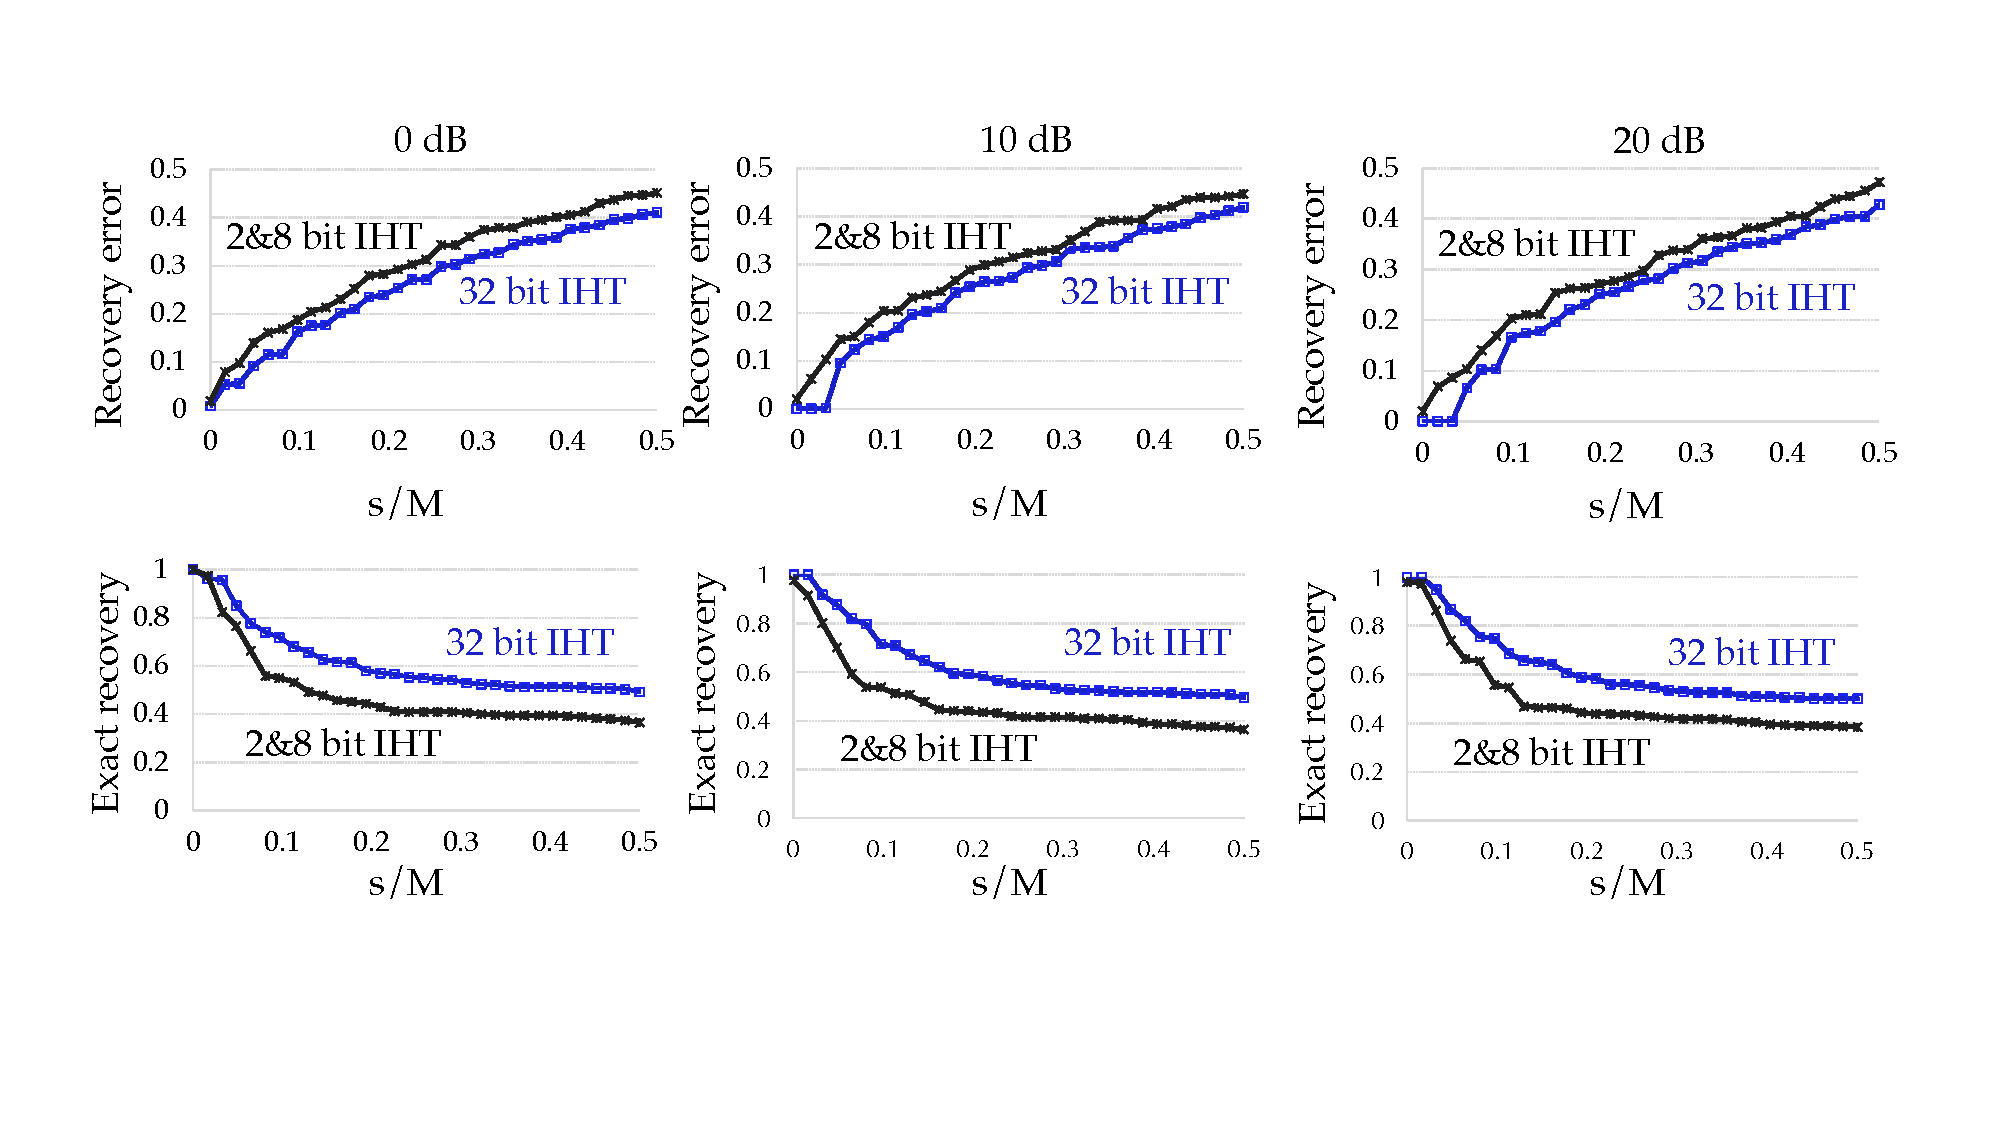
\includegraphics[width=1.02\columnwidth, angle=0]{figs/Gaussian.pdf}
\caption{Comparison of 2\&8 bit IHT to 32 bit IHT on Gaussian distributed data. The results are averaged over 100 realizations. Recovery error is calculated by $\| {\bf x}^{[n]} -{\bf x}^s \|_2/\|{\bf x}^s \|_2$ and exact recovery is given by the ratio between the cardinalities of recovered support and true support.}
\label{fig:iht_on_gaussian}
\vspace{-1em}
\end{figure}

\section*{Radio Interferometer Pipeline}\label{sec:astronomy}
Antennas at various locations on the ground records radio waves coming from the sources in space, and then send those to {\it interferometers} (correlator unit), which first estimate correlation between the time series-measurements so-called visibilities. Then the central processor estimates the sky image with a specified imaging technique, i.e., {CLEAN}~\citep{hogbom1974clean} and A(W)-projection~\citep{bhatganar2008ra}. 
\subsection*{Basic Data Model}

Let us start with the following modeling assumptions:~\citep{perley1999ra}

1. Celestial sources are in far field, the series emanating from sources and captured by the antennas are thus paralel,
  
2.  series emitted by celestial sources are narrow band zero mean circularly-symmetric complex Gaussian processes,
    
3.  series originating from different directions in the sky are uncorrelated.  
  
(1) follows from the assumption sources lie on a hypothetical sphere, the so-called celestial sphere. This implies that we can not measure how far the sources are.
 \vspace{3mm}
 
Let $\hat{s}(t,{\bf r})$ denote the series emitted by the source coming from the direction ${\bf r} \in \mathbb{S}^2$. (2), therefore, implies $\hat{s}(t,{\bf r}) \sim \mathbb{C}\mathcal{N}(0,I(\bf{r}))$ where $I(\bf{r})$ is the intensity of the source series emanating from direction {\bf r}. Given the center frequency $f_0 \in \mathbb{R}$, (2) yields the following baseband representation of $\hat{s}(t,{\bf r})$:
\begin{equation}
 s(t,{\bf r}) = \hat{s}(t,{\bf r})e^{j2\pi f_0t}.\label{baseband}
 \end{equation}
 
Note also that $\mathbb{E}[s(t,{\bf r}_1)s^*(t,{\bf r}_2)] =0$, $\forall {\bf r}_1, {\bf r}_2 \in \mathbb{S}^2$ follows from (3), where $*$ denotes the conjugate operator. 
The series coming from direction {\bf r} and recorded by antenna $i$ is thus given by:
\begin{equation}
x_i(t,{\bf r}) = s(t-\tau_{i}({\bf r}),{\bf r}) \label{ant_source}
\end{equation} 
 where $\tau_i({\bf r})$ denotes the time delay for the series reaching from the source to reach at the antenna $i$. Combining Eqn. \ref{baseband} and \ref{ant_source} we have
 \begin{equation}
 x_i(t,{\bf r}) = \hat{s}(t-\tau_{i}({\bf r}),{\bf r})e^{j2\pi f_0(t-\tau_{i}({\bf r}))}.
 \end{equation}
The above derivations concern merely a specific source. Let now focus on the series measured by the antenna $i$ coming from multiple sources (from all directions). It is then by the following integral:
\begin{equation}
x_i(t) = \oiint \displaylimits_{\mathbb{S}^2} \hat{s}(t-\tau_i({\bf r}), {\bf r})e^{j2\pi f_0(t-\tau_i({\bf r}))}d{\bf r}. \label{int_sour}
\end{equation}
 
As correlations between the antenna time-series are of special interest of imaging, let us have a closer look at the algebraic equations regarding the correlations. Recall that the source series coming from different directions in space are uncorrelated. Using this, we have the following closed-form expression:
 \begin{equation}
 \mathbb{E}[x_i(t)x_k(t)^*] = \oiint\displaylimits_{\mathbb{S}^2} \mathbb{E}[\hat{s}(t-\tau_i({\bf r}),{\bf r})\hat{s}^*(t-\tau_k({\bf r}),{\bf r})]e^{-j2\pi f_0 (\tau_i({\bf r})-\tau_k({\bf r}))}d{\bf r} \label{cross_corr}
 \end{equation}
 where $i$ and $k$ denote different antennas.
 By the assumption of (2), the series $\hat{s}(t,{\bf r})$ remains constant over the time shift we further have 
 \begin{equation}
 \mathbb{E}[x_i(t)x_k(t)^*] = \oiint\displaylimits_{\mathbb{S}^2} {I}({\bf r}) e^{-j2\pi f_0 (\tau_i({\bf r})-\tau_k({\bf r}))} d {\bf r} \label{cross_upt}
 \end{equation}
 where ${I}({\bf r})$ denotes the variance of the series emitted from direction {\bf r} referred to as sky image. We further have
%$\tau_{i,q} = \frac{1}{c} \langle {\bf r}_q,\lambda_0{\bf p}_i\rangle$\label{tau} 
%where ${\bf r}_q$ and ${\bf p}_i$ denote the direction of source $q$ and position of antenna $i$ expressed in the units of wavelengths $\lambda_0$, respectively.[]
\begin{equation}
\tau_{i}({\bf r}) = \frac{1}{c} \langle {\bf r}_{\text{norm}}, {\bf p}_i\rangle \label{tau}
\end{equation}

where ${\bf r}_{\text{norm}} = \frac{{\bf r}}{\| {\bf r}\|_2}$ and ${\bf{p}}_i$ denotes the position of antenna $i$.
The above relation together with Eqn. \ref{cross_upt} gives us that
\begin{equation}
 \mathbb{E}[x_i(t)x_k(t)^*] = \oiint\displaylimits_{\mathbb{S}^2} {I}({\bf r}) e^{-j2\pi \frac{f_0}{c} \langle {\bf r}_{\text{norm}},  \ {\bf p}_i -{\bf p}_k\rangle }d{\bf r}.\label{corr_f}
\end{equation}
Note that $\frac{f_0}{c} = \frac{1}{\lambda_0}$ where $\lambda_0$ is the wavelength of the observation, Eqn. \ref{corr_f} can be further simplified to the following equation:
\begin{equation}
 \mathbb{E}[x_i(t)x_k(t)^*] = \oiint\displaylimits_{\mathbb{S}^2} {I}({\bf r}) e^{-j2\pi \langle {\bf r}_{\text{norm}},  \ \frac{{\bf p}_i -{\bf p}_k}{\lambda_0}\rangle }d{\bf r}\label{corr_four}
\end{equation}
so-called {\bf measurement equation}.
\vspace{0.5em}

Consider now a specific region of interest centered around ${\bf r}_0$ and basis vectors $\hat{{\bf e}}_1$, $\hat{{\bf e}}_2$ and $\hat{{\bf e}}_3$ where $\hat{{\bf e}}_1$ points in the direction of rotation of the earth, $\hat{{\bf e}}_3$ denotes the direction of ${\bf r}_0$ and $\hat{{\bf e}}_2$ is perpendicular to $\hat{{\bf e}}_1$ and $\hat{{\bf e}}_3$. ${\bf r}$ can be therefore approximated to $r \approx l\hat{{\bf e}}_1 + m\hat{{\bf e}}_2 +1\hat{{\bf e}}_3$\footnote{More clearly; $ ({\bf r}-{\bf r}_0) + {\bf r}_0 \approx l\hat{{\bf e}}_1 + m\hat{{\bf e}}_2 +1\hat{{\bf e}}_3$.}. Similarly, $\frac{{\bf p}_i -{\bf p}_k}{\lambda_0}$ can also be expressed in terms of the basis vectors, i.e., $\frac{{\bf p}_i -{\bf p}_k}{\lambda_0} = u_{i,k}\hat{{\bf e}}_1+v_{i,k}\hat{{\bf e}}_2+w_{i,k}\hat{{\bf e}}_3$. Substituting these into Eqn. \ref{corr_four}, we get
\begin{equation}
 \mathbb{E}[x_i(t)x^*_k(t)] =   \iint\displaylimits_{K\subset \mathbb{R}^2} \frac{e^{-j2\pi w_{i,k} (\sqrt{1-l^2-m^2}-1)}}{\sqrt{1-l^2-m^2}} {I}(l,m)e^{-j2\pi (u_{i,k}l+v_{i,k}m)} \   dl\ dm \label{tangent_plane}
\end{equation}
where $K$ is the compact support of $I \in \mathbb{R}^2$. The above equation is called {\bf tangent plane measurement equation}.
\vspace{0.5em}

As indicated earlier, the field of view is small pointing ${\bf r}_0$, i.e., small $l$ and $m$. Hence $\frac{e^{-j2\pi w_{i,k} }}{\sqrt{1-l^2-m^2}-1} \sim 1$ and $\sqrt{1-l^2-m^2}$ term can be assumed to be constant. The above resulting representation can then be further simplified to the following:
\begin{equation}
 \mathbb{E}[x_i(t)x^*_k(t)] =   \iint\displaylimits_{K\subset \mathbb{R}^2} e^{-j2\pi w_{i,k}}{I}(l,m) e^{-j2\pi (u_{i,k}l+v_{i,k}m)} \   dldm.
\end{equation}
%the sources lie on a plane as well as the antennas.

{\bf{Key definition:}} The {\it{visibility}} function is defined by removing the constant phase $e^{-j2\pi w_{i,k}}$ as follows:
\begin{equation}
V(u, v) \stackrel{{\text{def}}}{=} \iint\displaylimits_{K\subset \mathbb{R}^2} {I}(l, m)e^{-j2\pi (ul+vm)}\ dldm.
\end{equation}

Therefore, each sample of this function is given by $V(u_{i,k}, v_{i,k}) = \mathbb{E}[x_i(t)x^*_k(t)]$ the so-called {\it{visibility}} measurement. 
\vspace{0.5em}

Remark that {\it{visibility}} equation is an integration of the product of sky intensity and a complex exponential over the unit sphere, which can be represented as a two dimensional Fourier transform. {\bf{Therefore, {{visibility}} function is equivalent to Fourier transform of the image I(l, m\bf )}}. This relation is known as van Cittert-Zernike theorem~\citep{perley1999ra}.  Consequently, the samples of $V(u,v)$ are sufficient information for sky image recovery where each baseline gives an approximate sample from Fourier transform of the sky image. This can be mathematically stated as follows:
\begin{equation}\label{visibility equation}
V_{i,k} \sim V(u_{i,k}, v_{i,k}) = \iint\displaylimits_{K\subset \mathbb{R}^2} {I}(l, m)e^{-j2\pi (u_{i,k}l+v_{i,k}m)}\ dl\ dm.
\end{equation}

Therefore, the sky image can be recovered by taking inverse Fourier transform of the non-uniformly samples visibility function so-called {\it dirty image} as follows:
\begin{equation}
I_d(l, m) = \mathcal{F}^{-1}\Big \{ \sum_{i, k} V(u, v) \delta (u-u_{i,k}, v-v_{i,k}) \Big \}.\label{meas_eq_non_beam}
\end{equation}

A closer look into the above equation reveals that {\it dirty image} is equivalent to
\begin{equation}\label{dirty_image}
I_d(l, m) = I(l, m)\ast I_{db}(l, m) 
\end{equation}
where 
\begin{equation}\label{dirty_beam}
I_{db}(l, m)= \sum_{i, k} e^{j2\pi(u_{i, k}l+v_{i, k}m)}
\end{equation}
is called {\it dirty beam} with $k$ baselines ((i, k) pairs with the previous notation), ${\bf I}(l, m)$ is the true sky map,  and $\ast$ denotes convolution operator.
\vspace{0.5em}

The imaging problem in radio astronomy can be viewed as reconstructing a sky image from estimates of its Fourier transform samples. Moreover, the problem is ill-posed as we have finite number of antennas thus the baselines. This can be tackled with up to some level by introducing a prior sky model. After having reviewed the basic data model and revealed how visibilities link to Fourier transform of the sky intensities, let us now focus on the data model from array series processing point of view. 
 \vspace{0.5em}
 
As widely used, we (very often astronomers as well) assume a point source model for the sky~\citep{veen2013ra, perley1999ra}. The series measured by the antenna $i$ denoted by $x_i(t)$ is given by:
 \begin{equation}\label{idare}
 x_i(t) = \sum_{q=1}^Q \hat{s}(t-\tau_{i,q},{\bf r}_q)e^{j2\pi f_0 (t-\tau_{i,q})}
 \end{equation} 
 where $\tau_{i,q}$ is the time delay at the antenna $i$ for source $q$ and $Q$ denotes the number of sources. 
 \vspace{0.5em}
 
Recall that the series $\hat{s}(t,r)$ remains constant over the time shift, i.e., $\hat{s}(t-\tau_{i,q},{\bf r}_q) = \hat{s}(t-\tau_{k,q},{\bf r}_q)$, $\forall i,k$ and hence Eqn. \ref{idare} can be simplified as follows:
\begin{equation}
\begin{split}
x_i(t) &\stackrel{(1)}{=} \sum_{q=1}^Q \hat{s}(t-\tau_{i,q},{\bf r}_q)e^{j2\pi f_0 (t-\tau_{i,q})}\\
&\stackrel{(2)}{=} \sum_{q=1}^Q \hat{s}(t, {\bf r}_q)e^{j2\pi f_0 (t-\tau_{i,q})}\\
&\stackrel{(3)}{=} \sum_{q=1}^Q \hat{s}_q(t)e^{j2\pi f_0 (t-\tau_{i,q})}
\end{split}
\end{equation}
where (1) and (2) follow from the arguments above. To simplify notation, we denote $\hat{s}(t,{\bf r}_q)$ by $\hat{s}_q(t)$ which leads (3).
By Eqn. \ref{tau}, we have
\begin{equation}\label{mudur}
x_i(t) = \sum_{q=1}^Q \hat{s}_q(t)e^{j2\pi f_0 (t- \langle {\bf r}_q,\lambda_0{\bf p}_i\rangle/c)}.
\end{equation}
 
Consider now that antenna series $x_i(t)$, $i\in \{ 1,...,L\}$ are concatenated in a vector ${\bf x}(t) \in \mathbb{C}^L$. Eqn. \ref{mudur} can be re-written as
 \begin{equation}
{\bf x}(t) = e^{j2\pi f_0 t} \sum_{q=1}^Q {\bf a}_q \hat{s}_q(t)\label{ind_xt}
\end{equation}
where $\bf{a}_q \in \mathbb{C}^L$ so-called {\it antenna steering vector} is given by
\begin{equation}\label{steering}
\bf{a}_q =
  \begin{bmatrix}
    e^{-j2\pi \langle {\bf r}_q, {\bf p}_1 \rangle}   \\
    e^{-j2\pi \langle {\bf r}_q, {\bf p}_2 \rangle}    \\
    \vdots \\
    e^{-j2\pi \langle {\bf r}_q, {\bf p}_L \rangle}   
  \end{bmatrix}
 \end{equation}
 towards source $q$.
 
Let ${\bf A} \in \mathbb{C}^{L\times Q}$ denote {\it antenna steering matrix} with each column given by individual {\it antenna steering vector} ${\bf a}_q$ and also $\hat{\bf{s}}(t)$ be vector of source series $\hat{s}_q(t)$, $q \in \{ 1,2,...,Q \}$. We then have following matrix product:
 \begin{equation}
 {\bf x}(t) = e^{j2\pi f_0 t}\bf{A} \hat{\bf{s}}(t).
 \end{equation}
 
 Up to now, we have introduced the data model under perfect conditions in means of noise. Real-life scenarios however are not that optimistic. Conversely, thermal noise usually has a big share in the series measured by the antennas. Let thus ${\bf n}(t) \in \mathbb{C}^L$ be the additive white Gaussian noise (AWGN) at the antennas. More realistic model for {\bf x}(t) in presence of noise can be as the following:
 \begin{equation}
 {\bf x}(t) = e^{j2\pi f_0 t}\bf{A} \hat{\bf{s}}(t) + {\bf n}(t)\label{x_t}
 \end{equation}
where ${\bf n}(t)$ is assumed to be independently drawn from the distribution $\mathbb{C} \mathcal{N}(0,\sigma_n^2 \bf{I}_L)$, $\sigma_n \in \mathbb{R}$ and ${\bf I}_L$ is $L\times L$ identity matrix. Moreover, the series emitted by the sources $\hat{{\bf s}}(t)$ are also modelled as stochastic processes where the parameters to be estimated, i.e., $\hat{{\bf s}}(t) \sim \mathbb{C}\mathcal{N}(0, {\bf \Sigma}_s)$ where ${\bf \Sigma}_s$ is the diagonal covariance matrix for the source series $\hat{{\bf s}}(t)$. 

Let ${\bf V}$ account for the visibility (cross-correlation) matrix. Then

\begin{equation}
\begin{split}
{\bf V} & = \mathbb{E}[{\bf x}(t){\bf x}^{\dagger}(t)]\\
& = \mathbb{E}[\big(e^{j2\puf_0t}{\bf A}\hat{\bf s}(t)\big)\big(e^{j2\puf_0t}{\bf A}\hat{\bf s}(t)\big)^{\dagger}]\\
& ={\bf A}{\bf \Sigma}_s{\bf A}^{\dagger} + {\bf \Sigma}_n.
    \end{split}
\end{equation}

\subsection*{Formation of ${\bf \Phi}$}
We first form a grid of sky map by ${\bf I}_{l, m} \in \mathbb{R}^{r\times r}$ for $l, m \in \{1, 2, ..., r \}$, where $r$ is the resolution of the map. Let ${\bf p}_{i, k} \in \mathbb{R}^2$ denote the two-dimensional distance between $i$'th and $k$'th antenna, and ${\bf r}_{l, m}\in \mathbb{R}^2$ stand for two-dimensional position of pixel in $l$'th row and $m$'th column of ${\bf I}$, respectively. 

Using Eqn.~\ref{visibility equation}, we can approximate the noisy visibilities by
%sky map ${\bf I}(l, m) \in \mathbb{R}^{r\times r}, $, where $r$ is the resolution of images, by
\begin{equation}\label{measurement_equation}
    {\bf V}_{i, k} = \sum_{l, m} {\bf I}_{l, m} e^{-j2\pi f_0 \langle{\bf p}_{i, k}, {\bf r}_{l, m}\rangle} + \delta_{i, k}.
\end{equation}

\begin{definition}
Let ${\bf A} \in \mathbb{K}^{M\times N}$ be a matrix, with field ${\mathbb{K}}$. The $vec(\cdot)$ operator is defined
\begin{equation*}
    {vec(\cdot)}: \mathbb{K}^{M\times N} \rightarrow \mathbb{K}^{MN}.
\end{equation*}
\end{definition}
\vspace{0.5em}

Using above definition we can reformulate Eqn.~\ref{measurement_equation} as follows.
\begin{equation}
    {\bf y} = {\bf \Phi}{\bf x} + {\bf e}
\end{equation}

with ${\bf y}, {\bf e} \in \mathbb{C}^{M}$, ${\bf \Phi} \in \mathbb{C}^{M\times N}$ and ${\bf x} \in \mathbb{R}^{N}$ such that ${\bf y} = vec({\bf V})$, ${\bf x} = vec({\bf I})$, ${\bf e} = vec(\boldsymbol{\Sigma}_n)$ and finally
\begin{equation}
    {\bf \Phi}_{z,w} = e^{-j2\pi f_0 \langle {\bf p}_{i, k}, {\bf r}_{l, m} \rangle } 
\end{equation}
where $z = i + L(k-1), \ \ i, k = \{1, 2, ..., L\}$ and $w = l + r(m-1), \ \ l, m = \{1, 2, ..., r\}$.
\vspace{0.5em}

Clear by its definition, the entries of ${\bf \Phi}$ have unity magnitude. Moreover, when ${\bf \Phi}$ is formed by using closely located antennas, the phase difference between the entries is even smaller, which suggests that, compressive sensing problem in radio inteferometry has the least desirable measurement matrix structure regarding the performance of $\ell_0$-minimization methods on such matrices. However, this will in turn be useful for our application: the bounds on $\gamma_{2s}$ and $\hat{\gamma}_{2s}$ will likely be satisfied.

\subsubsection*{How we satisfy conditions on Restricted Isometry Constants?}
Real-life problems usually lack of traditional RIP, that is, $\|{\bf \Phi}\|_2 < 1$. The scale-invariant feature of the measurement matrix used in normalized IHT however alleviates the RIP condition and imposes a fairly mild constraint in Eqn.~\ref{rip_lowprecision}, i.e., non-symmetric RIP. In a series of paper~\citep{blumensath2010niht, blumensath2012greedy}, CoSaMP is shown to perform markedly worse when the RIP condition fails. IHT, however, still preserves its near-optimal recoveries far beyond the region of RIP. %While this favors IHT over CoSaMP when applying to real-life problems, there is no rigid assumption imposed on $\ell_1$-minimization. Still \ref{rip} trivially holds.
Recall from the main paper that the step size $\hat{\mu}^{[n]}$ is required to counteract the scaling of $\hat{{\bf \Phi}}$ such that $\|\hat{\mu}^{0.5} \hat{\bf\Phi}\|_2^2 <1$ to ensure the convergence. 
The adaptive step size setting of normalized IHT yields the trivial bound on $\mu$ as~\citep{blumensath2012greedy}
\begin{equation}
   1/\hat{\beta}_{2s}^2\leq  1/\hat{\beta}_s^2 < \hat{\mu}^{[n]} < 1/\hat{\alpha}_s^2 \leq 1/\hat{\alpha}_{2s}^2.
\end{equation}
\begin{figure}[t!]
\centering
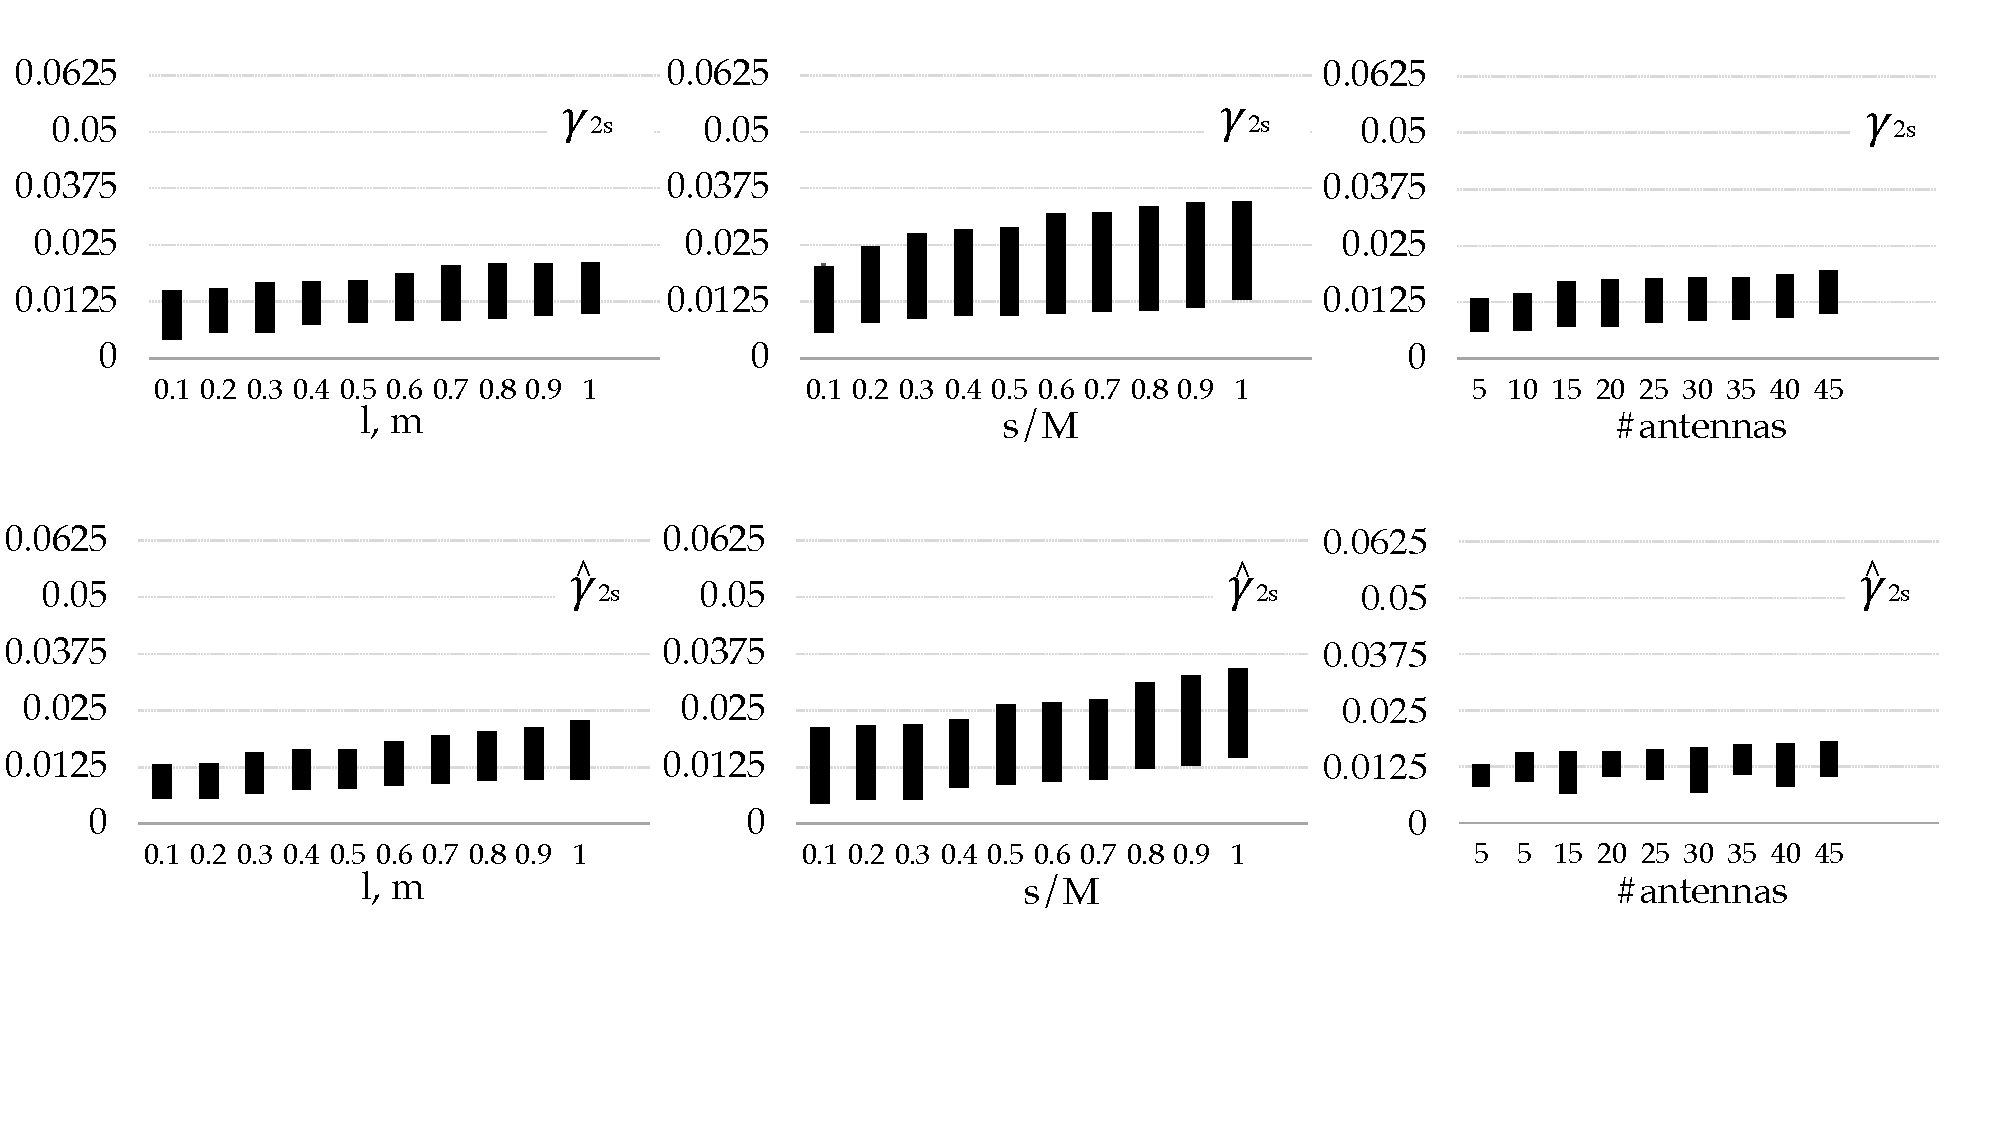
\includegraphics[width=1\columnwidth, angle=0]{figs/gamma.pdf}
\caption{The change of $\gamma_{2s}$ and $\hat{\gamma}_{2s}$ with grid boundaries {\it l} and {\it m}, the sparsity ratio $s/M$ and the number of antennas. For all cases, the conditions on $\gamma_{2s}$ and $\hat{\gamma}_{2s}$ are satisfied. For each box, 1000 realizations of ${\bf x}$ are drawn from a normal distribution and the largest and smallest $\|{\bf \Phi x} \|_2/\| {\bf x}\|_2$ is computed to estimate $\gamma_{2s}$, and this is repeated 100 times to have a numerical range of possible ${\gamma}_{2s}$ values. }
\label{fig:gamma}
\end{figure}

Convergence is trivial in low precision setting provided that $\hat{\mu}^{[n]}$ is chosen adaptively according to strategy introduced by~\citep{blumensath2010niht}. Regarding performance guarantees, however, in Theorem 3 we show that if $\gamma_{2s} = \beta_{2s}/\alpha_{2s}-1, \hat{\gamma}_{2s} = \hat{\beta}_{2s}/\hat{\alpha}_{2s}-1\leq 1/16$, then the recovery error inversely scales with $\beta_{2s}$ and $\hat{\beta}_{2s}$, which we can up-scale hence reduce the error. We previously sketch the values of $\beta_{2s}$ and $\hat{\beta}_{2s}$ for the current setting in our paper and show that they are large enough to diminish recovery error and no upscale is necessity in radio astronomy case. Yet, for provable guarantees, yet, we need to satisfy the conditions on $\gamma_{2s}$ and $\hat{\gamma}_{2s}$. Clearly, this cannot be done by re-scaling $\beta_{2s}$ and $\hat{\beta}_{2s}$ because $\alpha_{2s}$ and $\hat{\alpha}_{2s}$ will be scaled accordingly by the same weight. Therefore it remains to use a more sophisticated technique to achieve this. We claim that there exist possible deterministic transformations that can be applied on ${\bf \Phi}$. However, in radio astronomy, we have the flexibility to ensure the conditions on $\gamma_{2s}$ and $\hat{\gamma}_{2s}$ holds as follows. 
\vspace{0.5em}

Let us form a grid on $[l, m], \  \ l, m \in [-d, d]$ where the sky map is displayed. By changing $d$, we claim that the bounds on $\gamma_{2s}$ and $\hat{\gamma}_{2s}$ can be tuned. Given the antenna locations, we can compute ${\bf \Phi}$ that ensures the conditions with high probability. Fig.~\ref{fig:gamma} illustrates the numerical experiments conducted in the current setting where we recover the sky map with resolution of 256 pixels per axis. The numerical results suggest that these conditions in the certain settings and can be further refined with parameter $d$. Yet, everything comes with its own cost. The disadvantage of this strategy lies in the meaning of $d$, that is, $d$ limits the field of view the antennas observe. Luckily, it is not a practical concern as the limits of $d$ can be known a priori given number and the locations of antennas. Also, when we increase $d$ drastically to enlarge the field of view and no longer observe a sky source in the outer field, it already hints on the practical range of $d$ for the respective setting. In our setting, practical range of d is contained in $[0, 1]$. The conditions on $\gamma_{2s}$ and $\hat{\gamma}_{2s}$ are satisfied in our setting with high probability. The effect of antenna numbers and sparsity level are also illustrated in Fig.~\ref{fig:gamma}. Increase in the sparsity ratio $s/M$ and $d$ leads a slight increase in $\gamma_{2s}$ and $\hat{\gamma}_{2s}$. However, we can control this and adjust accordingly to satisfy the conditions. The values of $\gamma_{2s}$ and $\hat{\gamma}_{2s}$ are naturally satisfied in our settings, i.e., $\gamma_{2s}, \hat{\gamma}_{2s}\leq 1/16=0.0625$.
\subsection*{Inverse Fourier transform combined with CLEAN algorithm}
Referring to Eqn.~\ref{dirty_image} \& \ref{dirty_beam}, current imaging techniques first performs naive inverse Fourier transform of the visibilities such that
\begin{equation}
{\bf I}_{d}(l, m) = \sum_{i, j} V(u_{i, j}, v_{i, j})e^{j2\pi (u_{i, j}l+v_{i, j}m)}.
\end{equation}

%Location and flux intensities of the sources are estimated by the CLEAN algorithm.

CLEAN algorithm (a deconvolution algorithm) therefore takes the {\it dirty image} ${\bf I}_d(l, m)$ as input and outputs a sparse sky map by iteratively removing a fraction\footnote{so-called {\it loop gain} $\leq 0.3$} of the highest peak convolved with the {\it dirty beam} {\bf I}${}_{db}$(l, m). 




\begin{figure}[t!]
\centering
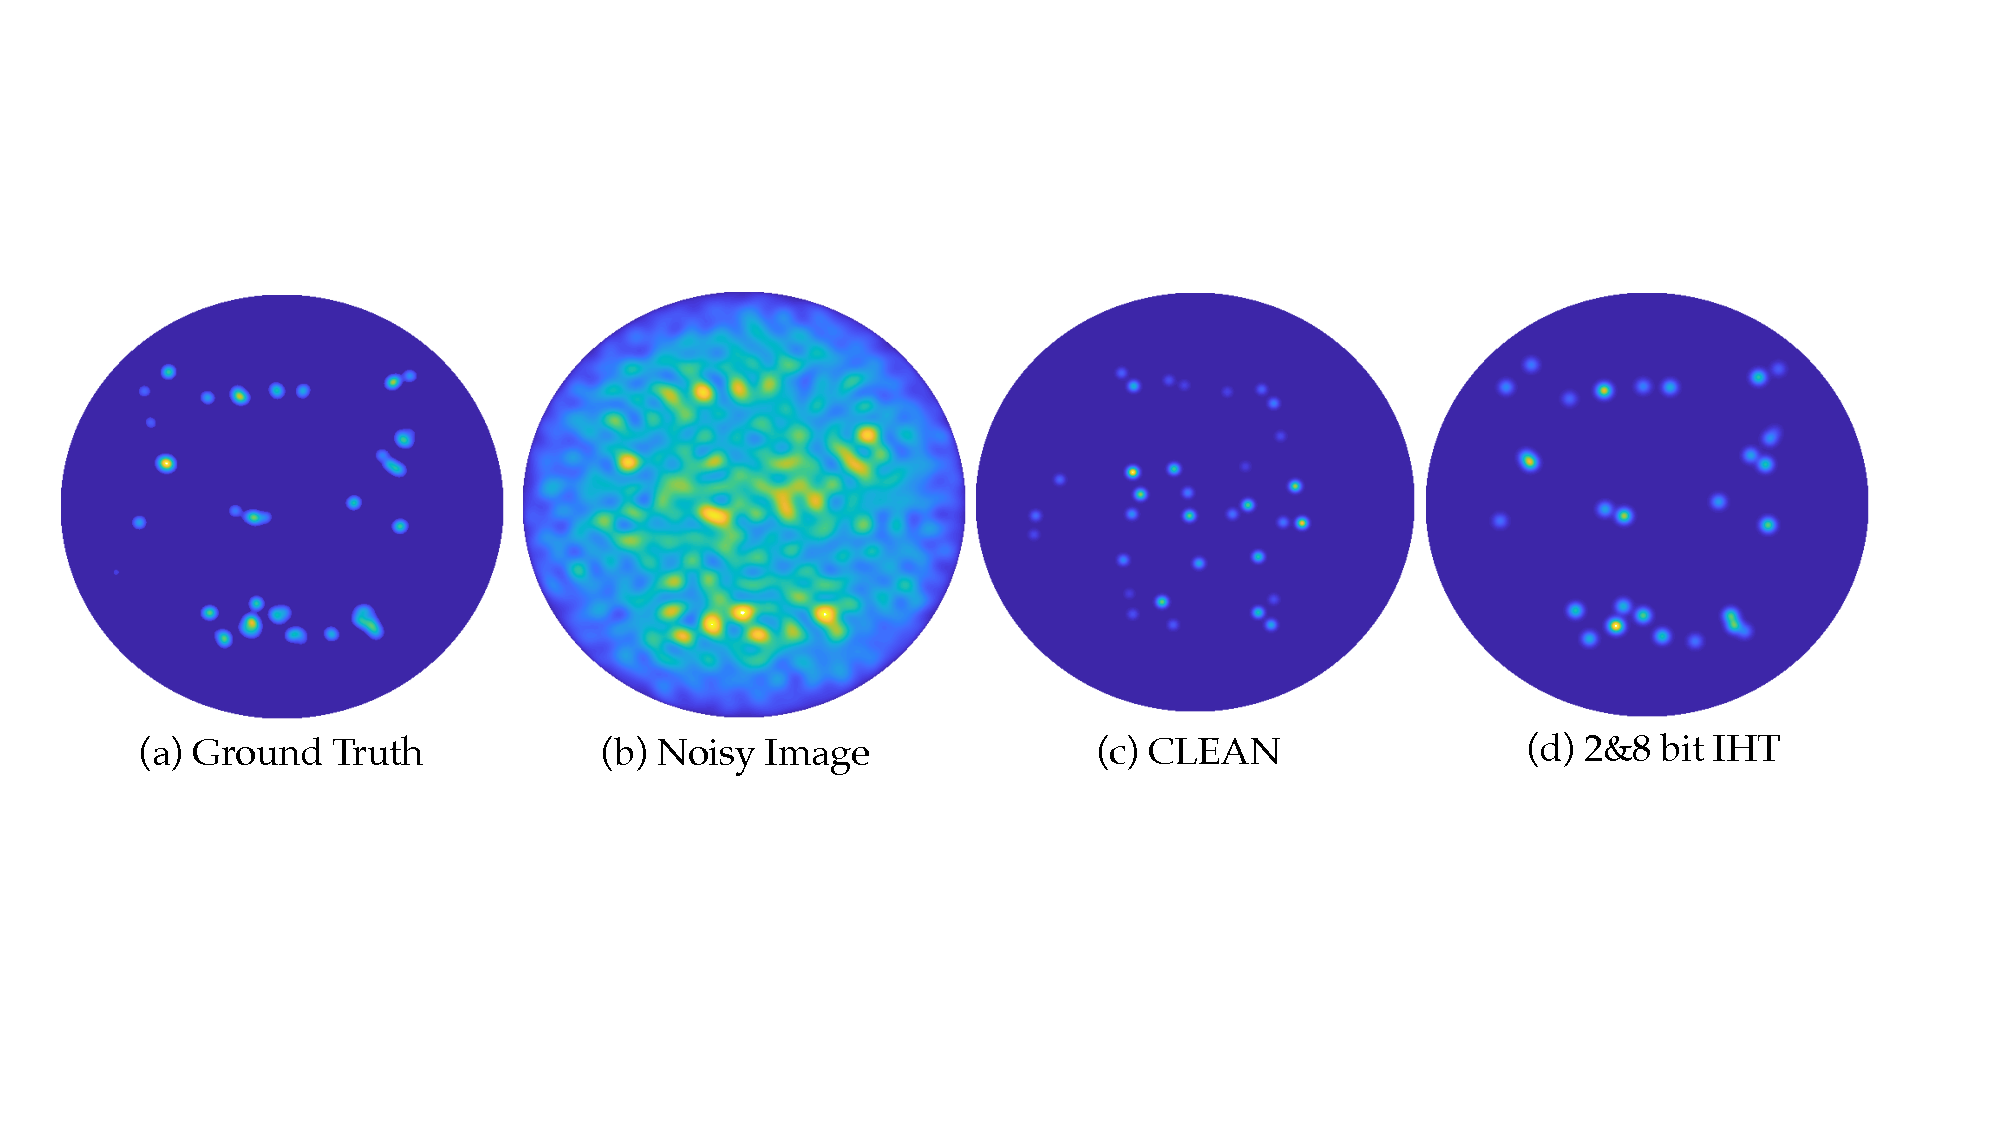
\includegraphics[width=1\columnwidth, angle=0]{figs/clean.pdf}
\caption{Comparison of 2\&8 bit IHT to CLEAN Algorithm. The CLEAN mostly captures the noise artefacts as actual sources unlike IHT.}
\label{fig:clean}
\end{figure}
Recall from the discussions in the main paper that noise in receivers is far stronger than the weak incoming signals thus low SNR at the antenna level results, i.e., usually ranged from -5 to 5 dB. In Fig.~\ref{fig:clean}, we apply the CLEAN algorithm to the LOFAR data set we use throughout the main paper, where SNR is computed nearly 0 dB. This particular experiment states that the CLEAN algorithm notably underperforms in the presence of significant noise. This undesirable property is yet not surprising. A careful look into the the algorithmic steps, it apparently matches also to the noise artefacts in the image considering them as a point source. This can also be justified mathematically: we designed the problem such that an execution of {CLEAN} corresponds to the first iteration recovery of IHT, which interprets our numerical results. 

Computationaly, the CLEAN requires a 2D Fourier inversion and deconvolution per iteration thus the operational expense of the method is relatively higher compared to those of IHT and CoSaMP. 



\bibliography{Auxiliaries/Supplementaries/references}
\bibliographystyle{Auxiliaries/Supplementaries/icml2018}


\end{document}
